\documentclass[a4paper]{scrartcl}
\usepackage{ngerman, amsmath, amssymb, esvect, graphicx, multirow, braket, dsfont, rotating, pstricks, pst-all, marvosym, nicefrac, longtable}
\usepackage{pst-pdf}
\usepackage[squaren]{SIunits}
\usepackage[utf8]{inputenc}

\usepackage{latexki}
%\lecturer{}
\semester{Sommersemester 2009}
\scriptstate{complete}

\newenvironment{aaufz}
	{\renewcommand{\labelenumi}{\alph{enumi})}
   \renewcommand{\labelenumii}{\alph{enumii})}
   \begin{enumerate}}
  {\end{enumerate}}

\newenvironment{iaufz}
	{\renewcommand{\labelenumi}{(\roman{enumi})}
   \renewcommand{\labelenumii}{(\roman{enumii})}
   \begin{enumerate}}
  {\end{enumerate}}

\newenvironment{1aufz}   			
	{\renewcommand{\labelenumi}{\arabic{enumi}.)}
	 \renewcommand{\labelenumii}{\arabic{enumii}.)}
   \begin{enumerate}}
  {\end{enumerate}}

\newcommand{\NN}{\ensuremath \mathbb{N}}
\newcommand{\ZZ}{\ensuremath \mathbb{Z}}
\newcommand{\QQ}{\ensuremath \mathbb{Q}}
\newcommand{\RR}{\ensuremath \mathbb{R}}
\newcommand{\CC}{\ensuremath \mathbb{C}}


\newcommand{\dOne}{\ensuremath \mathds{1}}

\newcommand{\dd}{\ensuremath \, \mathrm{d}}
\newcommand{\eps}{\ensuremath \varepsilon}
\renewcommand{\phi}{\ensuremath \varphi}
\renewcommand{\Im}{\ensuremath \mathrm{Im}}
\renewcommand{\Re}{\ensuremath \mathrm{Re}}
\newcommand{\tr}{\ensuremath \mathrm{tr} \, }
\newcommand{\matr}[1]{\begin{pmatrix} #1 \end{pmatrix}}
\newcommand{\eqn}[1]{\begin{align} #1 \end{align}}
\newcommand{\eqnnon}[1]{\begin{align*} #1 \end{align*}}
\newcommand{\spl}[1]{\begin{split} #1 \end{split}}

\parindent 0pt
\parskip 6pt

\begin{document}

\title{Theoretische Physik D: Quantenmechanik I}
\date{Sommersemester 2009}
\maketitle
\tableofcontents
\section{Grundbegriffe}

Die klassische Physik beschreibt folgende Ph"anomene nicht korrekt \ldots
\begin{aaufz}
	\item \ldots in der Physik makroskophischer Systeme
	\begin{itemize}
		\item Energieverteilung der Schwarzk"orperstrahlung
		\item spezifische W"arme bei niedrigen Temperaturen
		\item Kondensation
		\item Suprafluidit"at
		\item Koh"asion von Festk"orpern und Fl"ussigkeiten
		\item Gitterschwingungen (Phononen)
		\item elektrische Leitf"ahigkeit (Normal-, Halbleiter-, Supraleiter-)
		\item Ferromagnetismus
	\end{itemize}
	\item \ldots in der Atom- und Molek"ulphysik
	\begin{itemize}
		\item Gr"o"se und Stabilit"at der Atome
		\item Ladungsverteilungen
		\item Spektren
		\item Wechselwirkung mit Licht (z.B. Photoeffekt)
		\item Molek"ulschwingungen 
		\item chemische Bindungen (z.B. Van-der-Waals-Bindung)
	\end{itemize}
	\item \ldots in der Kernphysik
	\begin{itemize}
		\item Gr"o"se und Stabilit"at der Kerne
		\item Wechselwirkung von $\gamma$-Strahlen mit Kernen 
		\item radioaktiver Zerfall
		\item Kernspaltung und -fusion
	\end{itemize}
	\item \ldots in der Elementarphysik
	\begin{itemize}
	\item Masse, Ladung, Drehimpuls, magnetisches Moment der Elementarteilchen
	\item Wechselwirkung mit Strahlung (Comptoneffekt)
	\item Streuung, Zerfall
	\item Teilchenerzeugung
	\end{itemize}
\end{aaufz}
Die Quantenmechanik (QM) bildet die Grundlage des Verst"andnisses dieser Ph"anomene.

\subsection{Ursprung der Quantenphysik}



\begin{tabular}{l p{400pt}}
1901:	& 
Planck: Schwarzk"orperstrahlung 
  \begin{align}
  E = h \nu = \hbar \omega, \  \hbar = \frac{h}{2 \pi}
  \end{align}
  $h \approx 6,6 \cdot 	10^{-35} \joule \second= 4 \cdot 10^{-15} \electronvolt \second$
\end{tabular}
\\

\begin{figure}[h]
\centering
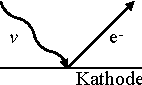
\includegraphics{001Photoeffekt} 
\caption{Photoeffekt}
\label{Photoeffekt1}
\end{figure}

\begin{tabular}{l p{400pt}}
1905: &
Deutung des Photoeffekts (\ref{Photoeffekt1}) durch Einstein: 
$$E = h\nu - W$$
$W$: Austrittsarbeit, $E$: unabh"angig von der Intensit"at $I$ des Lichts. Photon mit Energie $E = h \nu$, $I \propto $ Zahl der Phtononen.
\end{tabular}
\\

\begin{figure}[h]
\centering
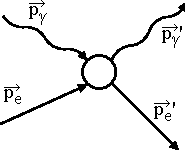
\includegraphics{002Comptoneffekt} 
\caption{Comptoneffekt}
\label{Comptoneffekt1}
\end{figure}

\begin{tabular}{l p{400pt}}
1924: &
Compton-Effekt (\ref{Comptoneffekt1}): Impuls der Photonen: $0 = mc^2 = \sqrt{ E^2 - \vv p^2 c^4 }$
\begin{align}
h c \vert \vv k \vert = \hbar \omega = E = \vert \vv p \vert c \ \Longrightarrow \ \vert \vv p \vert = \hbar \vert\vv k \vert,
\end{align}
$\vv k$: Wellenvektor
\end{tabular}
\begin{align*}
E_\gamma + E_e & = E_\gamma' + E_e' \\
\vv p_e + \vv p_\gamma & = \vv p_e' + \vv p_\gamma'
\end{align*}
\\
\begin{figure}[h]
\centering
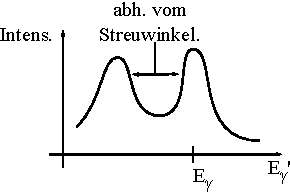
\includegraphics{002Intensitat} 
\label{002Intensitat}
\end{figure}

\begin{tabular}{l p{400pt}}
& \emph{klassische Physik:} $e^-$ wird kontinuierlich beschleunigt, $\Delta E$ (aus Dopplereffekt) w"achst mit Zeit. \\
\\
1923: & Broglie: Alle Teilchen haben Wellennatur
$$\vv p = \hbar \vv k \ \leadsto \  \lambda = \frac{\hbar}{ \vert \vv p \vert } \ \mathrm{ deBroglie-Wellenl"ange}$$
$\lambda \approx \frac{12,2}{\sqrt{ E/ \electronvolt}} \angstrom$ (nichtrelativistische Teilchen)
\\
1927: & Davisson, Gerner: $e^-$ an Einkristall gestreut, Laue-Diagramm \\
1928: & G.P. Thomsen / Rupp: Debye-Scherrer \\
1905: & Rydberg-Ritz-Formel f"ur Spektrallinien des H-Atoms
$$\nu = R\left( \frac1{n^2} - \frac1{m^2} \right), \quad n<m \in \NN$$
$R$: Rydberg-Konstante \\
1913: & N. Bohr: Energie-Quantisierung: $$E_n = - h \frac{R}{n^2}, \ n \in \NN.$$
Bohr-Sommerfeld-Quantisierung: klassische Bahn des $e^-$ um Atomkern, Hamilton-Funktion 
$$H(p,q) = \mathrm{const.} \quad \underbrace{\oint p \dd q}_{(*)} = nh, \ n = 1,2,3, \ldots$$
$(*) = $ Bahn im Phasenraum
\end{tabular}

\subsection{Zust"ande, Observable, Operatoren}

{
\begin{center}
\begin{tabular}{l  l}
klassisch. & QM \\
\hline
Welle & \multirow{2}{*}{ $\Big\}$ Zustand } \\
Teilchen
\end{tabular}
\end{center}
Photon mit Wellenzahlvektor $\vv k$ und Polarisation $\varepsilon \in \{ \varepsilon_x, \varepsilon_y \}$:
\begin{align}
\mathrm{Zustand:} \ \Ket{ \vv k, \epsilon}, \quad \vv p = \hbar \vv k, \ E= \hbar c \vert \vv k \vert
\end{align}
Nur Polarisation betrachet $\leadsto$ Doppelbrechender Kristall: Kalkspat

\begin{center}
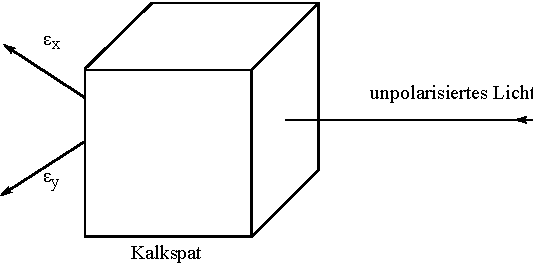
\includegraphics{003Kalkspat}
\end{center}
Polarisationsfilter $P_\varphi$:
\begin{center}
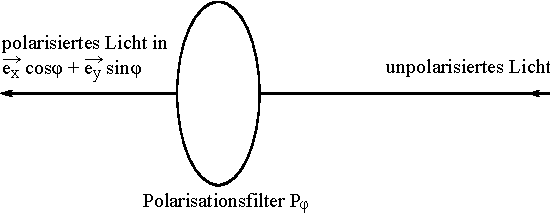
\includegraphics{003Polarisationsfilter1}
\end{center}
$P_x := P_{\varphi = 0}, \ P_y := P_{\varphi = \frac\pi2}$
\begin{center}
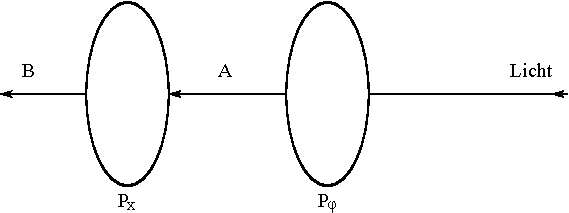
\includegraphics{003Polarisationsfilter2}
\end{center}
Beobachtung: Intensit"at ist bei $B$ gegen"uber $A$ um $\cos^2 \varphi$ abgeschw"acht. Das entspricht dem \emph{klassischen Wellenbild}. \\
\emph{Teilchenbild}: K"onnte die Photonenenergie abgeschw"acht sein? Nein: $E = h \omega$ ist gleichgeblieben. \\
\emph{statistische Interpretation:} 
Die Wahrscheinlichkeit, dass ein in $\varphi$-Richtung polarisiertes Photon $P_x$ passiert, ist $\cos^2 \varphi$.

Kalkspat:
\begin{center}
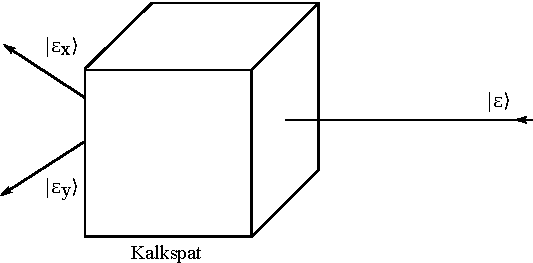
\includegraphics{003Kalkspat2}
\end{center}
Komponenten-Zerlegung:
\begin{align}
\Ket{ \varepsilon } = \alpha \Ket{ \varepsilon_x } + \beta \Ket{ \varepsilon_y}
\end{align}
Zust"ande bilden einen komplexen Vektorraum $\mathcal H$. Im Fall von Polarisationszust"anden gilt 
\begin{align}
\dim \mathcal{H} = 2.
\end{align}Zustandsvektroren nennt man auch \emph{Kets}. Es beschreibe $\Ket{ \varepsilon_\varphi }$ den Zustand eines in $\vv e_x \cos \varphi + \vv e_y \sin \varphi$ Richtung liniear polarisierten Photons.
\begin{center}
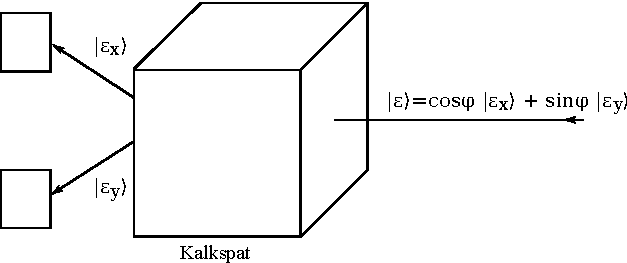
\includegraphics{004Kalkspat}
\end{center}
Beobachtungen:
\begin{itemize}
\item Es klickt entweder $D_x$ oder $D_y$
\item Welcher Detektor anspricht ist nicht vorhersehbar
\item Wiederholt man das Experiment oft, so findet man, dass bei $N$ Verscuhen $D_x$ etwa $N \cos^2 \varphi$ und $D_y$ etwa $N \sin^2\varphi$ anspricht.
\end{itemize}
Die Polarisationsfilter und der Kalkspatkristall vermitteln Abbildungen $\mathcal H \longrightarrow \mathcal H$, z.B.
\begin{align}
P_x: \Ket{ \varepsilon_\varphi } = \cos \varphi \Ket{ \varepsilon_x } + \sin \varphi \Ket{ \varepsilon_y } \longmapsto \cos \varphi \Ket{ \varepsilon_x }
\end{align}
Man schreibt:
\begin{align}
P_x \Ket{\varepsilon_\varphi } = \Ket{ P_x \varepsilon_\varphi} = \cos \varphi \Ket{ \varepsilon_x }
\end{align}
$P_\varphi$ ist Operator auf dem Vektorraum $\mathcal H$:
\begin{align}
P_\varphi: 
\left\{ 
\begin{array}{l l}
P_\varphi \Ket{\varepsilon_x } & = \cos \varphi \Ket{\varepsilon_\varphi} \\
P_\varphi \Ket{\varepsilon_y } & = \sin \varphi \Ket{\varepsilon_\varphi} 
\end{array}
\right\}
\end{align}
Es gilt:
\begin{align}
\begin{split}
P_\varphi \Ket{ \varepsilon_\varphi} & = P_\varphi \Big[ \cos \varphi \Ket{ \varepsilon_y } + \sin \varphi \Ket{ \varepsilon_y } \Big]  \\
& =  \cos \varphi P_\varphi \Ket{ \varepsilon_x } + \sin \varphi P_\varphi \Ket{ \varepsilon_y }  \\
& = \cos^2\varphi \Ket{\varepsilon_\varphi } + \sin^2 \varphi \Ket{ \varepsilon_\varphi }  \\
& = \Ket{ \varepsilon_\varphi } 
\end{split} \tag{9 + 10} 
\end{align}

\setcounter{equation}{10}
\subsubsection*{Mathematischer Exkurs}
Allgemein definieren wir f"ur $\dim \mathcal H = N < \infty$:
\begin{1aufz}
\item \emph{Skalarprodukt}:  Eine Abbildung $\mathcal H \times \mathcal H \longrightarrow \CC$, $( \Ket{ \psi }, \Ket{ \chi} ) \longmapsto \Braket{ \psi | \chi}$ mit:
\begin{align}
\Braket{\psi | \lambda_1 \chi_1 + \lambda_2 \chi_2} & = \lambda_1 \Braket{ \psi | \chi_1} + \lambda_2 \Braket{\psi  \chi_2}, \\
\Braket{ \psi | \chi }  & = \overline{ \Braket{ \chi | \psi }}, \\
\Braket{ \psi | \psi } & \begin{cases} = 0, &\Ket{ \psi } = 0, \\ > 0, & \Ket{\psi} \neq 0. \end{cases}
\end{align}
$\Vert \Ket{ \psi } \Vert := \sqrt{ \Braket \psi | \psi }$ hei"st \emph{Norm} von $\Ket{\psi}$.
Gilt $\Braket{\psi | \chi} = 0$, so hei"sen $\Ket \psi$ und $\Ket \chi$ \emph{orthogonal}.
\item \emph{Orthonormalbasis (ONB)}: Eine endliche Teilmenge $\set{ \Ket{e_i}, \ldots \Ket{e_N} } \subset \mathcal H$ mit
\begin{align}
\Braket{e_i | e_j} = \delta_{ij}
\end{align}
\item \emph{Linearer Operator}: Eine Abbildung $A: \mathcal H \longrightarrow \mathcal H$, $\Ket{\psi } \longmapsto \Ket{ A \psi } = A \Ket{ \psi}$ mit
\begin{align}
A \Ket{ \lambda_1 \psi_1 + \lambda_2 \psi_2} = \lambda_1 \Ket{A \psi_1} + \lambda_2 \Ket{A \psi_2}
\end{align}
\item \emph{Zu $A$ hermitesch konjugierter (oder adjungierter) Operator}: Ein linearer Operator $A^\dagger: \mathcal H \longrightarrow \mathcal H$ mit
\begin{align}
\braket{ \chi | A \psi } & = \braket{ A^\dagger \chi | \psi }.
\end{align}
\item Ein \emph{hermitescher (oder selbstadjungierter Operator $A$} ist ein Operator mit 
\begin{align}A = A^\dagger\end{align}
\item \emph{Eigenket (oder Eigenvektor) von $A$}: Ein Ket $\Ket{ \psi_\lambda}$ ($\lambda \in \CC$), mit
\begin{align}
A \Ket{ \psi_\lambda} = \lambda \Ket{\psi_\lambda} \label{18}
\end{align}
\item Existiert ein Operator $A^{-1}$, so dass
\begin{align}
A^{-1} A \Ket{\psi} = A A^{-1} \Ket{\psi}, \quad \Ket{\psi } \in \mathcal{H}
\end{align}
gilt, so ist $A$ \emph{invertierbar} und $A^{-1}$ hei"st der \emph{zu $A$ inverse Operator.}
\item Gilt $U^{-1} = U^\dagger$ (d.h. $U^\dagger U = U U ^\dagger = \dOne$), so hei"st $U$ \emph{unit"ar}. In diesem Fall gilt also:
$$\braket{ U \chi | U \psi } = \braket{ \chi | U^\dagger U | \psi } = \braket{ \chi | \psi}$$
\item \emph{Matrixdarstellung:} Betrachte eine ONB $\set{ \ket {e_1}, \ldots \ket {e_n} }$.
\begin{align} a_{ij} & := \braket { e_i | A | e_j }, \quad 1 \leq i,j \leq N \end{align}
definiert die Matrixdarstellung $a = (a_{ij})_{ij}$ von $A$ bzgl. $\set{ \ket {e_1}, \ldots \ket {e_n} }$.
\end{1aufz}
Eigenschaften dieser Objekte:
\setcounter{equation}{21}
\begin{aaufz}
\item Dreiecksungleichung:
\setcounter{enumi}{1}
\begin{align}
\Vert \Ket{\chi} + \Ket{\psi} \Vert & \left. \begin{cases} <, & \ket{ \chi}, \ket{ \psi} \mathrm{\ l.u.}  \\ =, & \ket{\chi}, \ket{\psi} \mathrm{\ l.abh.} \end{cases} \right\} \Vert \Ket{\chi} + \Vert \Ket{\psi}
\end{align}
\item Schwarzsche Ungleichung:
\begin{align} \vert \braket{ \psi | \chi } \vert \leq \Vert \ket{ \psi } \Vert \cdot  \Vert \ket{\chi } \Vert \end{align}
\item Mit $A$ und $B$ ist auch $\lambda_1 A + \lambda_2 B$ ein linearer Operator, wobei
$$( \lambda_1 A + \lambda_2 B) \ket{ \psi } := \lambda_1 \ket{ A \psi} + \lambda_2 \ket{B \psi}$$
\item F"ur $AB$ definiert durch $(AB) \ket{ \psi} = A (B \ket \psi)$, gilt i.A. $AB \neq BA$.
\item Gilt in einer ONB $\set{ \ket{e_1}, \ldots, \ket{e_n} }$
\begin{align}
\ket \psi = \sum_{n=1}^N c_n \ket {e_n}, \quad \ket \xi = \sum_{k=1}^N d_k \ket {e_k}, 
\end{align}
so folgt
\begin{align}
\begin{split}
\braket{ \chi | A | \psi } & = \sum_{k,n =1}^N d_k^* c_n \underbrace{\braket{ e_k | A | e_n}}_{=a_{kn}} \\
& = d^\dagger a c
\end{split} \label{25}
\end{align}
mit $$c=(c_1, \ldots, c_n)^\dagger, \quad d = (d_1, \ldots, d_n)^\dagger.$$
\item Aus \ref{25} folgt: \label{f}
\begin{itemize}
\item $a^{-1}$ ist Matrixdarstellung von $A^{-1}$,
\item $a^\dagger$ ist Matrixdarstellung von $A^\dagger$
\item $ab$ ist Matrixdarstellung von $AB$
\item mit $\ket{ \psi_\lambda } = \sum_{n=1}^N l_n \ket{e_n}$ in \ref{18} ist $l = (l_1, \ldots, l_n)^\dagger$ EV von $a$ zum Eigenwert $\lambda$.
\end{itemize}
\item Unit"arer Basiswechsel: $U^\dagger U = \dOne$, $\ket{e_i'} := U \ket{e_i}$. 
\begin{align*}
\Longrightarrow \braket{ e_j' | e_i' } & = \braket{ U e_j | U e_i } \\ 
& = \braket {e_j | \underbrace{U^\dagger U}_{= \dOne} | e_i } \\
& = \braket { e_j | e_i } = \delta_{ij}
\end{align*}
$\Longrightarrow \set{ \ket{ e_1'}, \ldots, \ket{e_n'}}$ ist ONB.

Wegen $f)$ haben hermitesche Operatoren $A$ dieselben Spektraleigenschaften, wie hermitesche Matrizen: (26)
\begin{iaufz}
\item Es gibt ONB aus Eigenkets $\set{ \ket{e_1}, \ldots, \ket{e_n}}$ und
\item alle EW sind reell.
\end{iaufz}
\setcounter{equation}{26}
\end{aaufz}
Eigenschaft (i) schreibt man "ublicherweise als 
\begin{align}
A = \sum_{j=1}^N \lambda_j \ket {e_j} \bra{e_j}.
\end{align}
Die zugeh"orige Matrix ist $a = \sum_{j=1}^N \lambda_j e^{(j)}  {e^{(j)}}^\dagger$, wobei $e^{(j)} = (e_1^{(j)}, \ldots, e_N^{(j)})^\dagger$ EV von $a$ zum EW $\lambda_j$ ist.

Dabei ist $P_j = \ket{e_j} \bra{e_j}$ ein Projektionsoperator:
\begin{align}
P_j \ket{\psi} & = \ket {e_j} \braket{ \psi| e_j}  = \braket{ \psi | e_j} \ket{e_j}, \\
\Longrightarrow P_j^2 & = \ket{e_j} \braket{e_j | e_j } \bra{e_j} = \ket{e_j} \bra{e_j} = P_j \notag
\end{align}
\begin{align}
P_j^\dagger & = P_j \Longleftarrow \Big[ a \ket{\psi}\bra{\chi} \Big]^\dagger = \alpha^* \ket{\chi} \bra{\psi}, \ \alpha \in \CC
\end{align}
Zuordnung:
\begin{align}
\mathrm{
\begin{tabular}{c c c}
ket $\ket{\psi}$ & \multirow{2}{*}{$\leftrightarrow$} & bra $\psi$ \\
Spaltenvektor $c$ & & Zeilenvektor $c^\dagger$
\end{tabular}
}
\end{align}
Aus (6) und (8) finden wir f"ur unsere Polarisationsoperatoren:
$$P_\varphi^2 = P_\varphi, \ P_\varphi^\dagger = P_\varphi \ \Longrightarrow P_\varphi \mathrm{ \ Polarisationsoperator}$$
\begin{center}
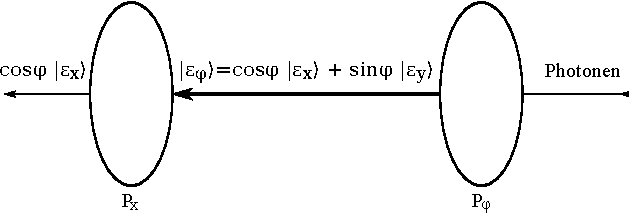
\includegraphics{030Polarisationsfilter}
\end{center}
\emph{Statistische Interpretation:} Wahrscheinlichkeit, dass f"ur $\ket{ \varepsilon_\varphi}$ die Polarisation $P_x$ gemessen wird ist 
\begin{align}
W_x & = \cos^2 \varphi 
 \stackrel{(17)}= | \braket {\varepsilon_x | \varepsilon_y } |^2 
 \stackrel{(21)}= \braket{ \varepsilon_\varphi | \varepsilon_x} \braket{ \varepsilon_x | \varepsilon_\varphi} 
 = \braket{ \varepsilon_\varphi | P_y | \varepsilon_\varphi}
\end{align}
wobei die Normierung $\braket{ \varepsilon_\varphi | \varepsilon_\varphi } = 1$ verwendet wird.

Ersetzt man $P_x$ durch $P_y$, so findet man 
\begin{align}
W_y = \sin^2 \varphi = \braket{ \varepsilon | P_y | \varepsilon_\varphi},
\end{align}
also
\begin{align}
W_x + W_y = 1, \quad P_x + P_y = \dOne \ \mathrm{und} \ P_xP_y = P_yP_x = 0.
\end{align}
(33) motiviert die 

\subsubsection*{Messpostulate der QM:}

\begin{iaufz}
\item Observable (= messbare physikalische Gr"o"sen) werden durch selbstadjungierte Operatoren beschrieben.
\item Wiederholt man eine Messung mehrfach an im Zustand $\ket \psi$ pr"aparierten Teilchen, so ist der Mittelwert der durch den Operator $A$ beschriebenen Observable durch den Erwartungswert von $A$ im Zustand $\ket \psi$
\begin{align}
W & = \frac{ \braket{ \psi | A | \psi }}{ \braket { \psi | \psi }}
\end{align}
gegeben
\item Die statistische Varianz der wiederholten Messungen ist
\begin{align}
\begin{split}
\sigma^2 & = 
\frac{ 
\braket{ \psi | (A - W \dOne)^2 | \psi }}
{ \braket{ \psi | \psi }} \\
& = 
\frac{ 
\braket{ \psi | A^2 | \psi} - 2 W \overbrace{ \braket{ \psi | A | \psi }}^{=W} + W^2 \braket{ \psi | \psi}}{\braket{ \psi | \psi}} \\
& = \frac{ \braket{ \psi | A^2 | \psi } - \braket{ \psi | A | \psi }^2}{\braket{ \psi | \psi }}.
\end{split}
\end{align}
Die Stndardabweichung $\sigma := \sqrt {\sigma^2}$ hei"st Unsch"arfe von $A$ im Zustand $\ket \psi$.

Kurzschreibweise:
\begin{align}
\begin{split}
\braket A & := W, \\
\Delta A & := \sigma.
\end{split}
\end{align}
\end{iaufz}
Im Fall der Polarisation $P_x$ sind die m"oglichen Messwerte $0$ (kein Ansprechen des Detektors) und $1$ (Detektor spricht an).
\begin{align}
\braket {P_x} & = \braket { \varepsilon_\varphi | P_x | \varepsilon_\varphi } = \cos^2 \varphi, \\
(\Delta P_x )^2 & = \braket { \varepsilon_\varphi | P_x^2 | \varepsilon_\varphi } - \cos^4 \varphi \notag \\
& = \cos^2 \varphi - \cos^4 \varphi \notag \\
& = \cos^2 \varphi \sin^2 \varphi \notag \\
& = \frac14 \sin^2(2 \varphi)
\end{align}

\begin{tabular}{l l p{300pt}}
$\varphi=0$ &  $\Delta P_x = 0$ &  $\ket { \varepsilon_{\varphi = 0}} = \ket { \varepsilon_x }$ ist Zustand minimaler Unsch"arfe (EV von $P_x$ zum EW 1) \\
$\varphi = \frac \pi 2$ & $\Delta P_x = 0$ & $\ket {\varepsilon_{\varphi = \frac \pi 2}} = \ket{ \varepsilon_y}$ \\
$\varphi = \frac \pi 4$ & $\Delta P_x = \frac12$ & Zustand maximaler Unsch"arfe
\end{tabular}

\subsubsection*{Zirkular polarisierte Photonen}

\begin{center}
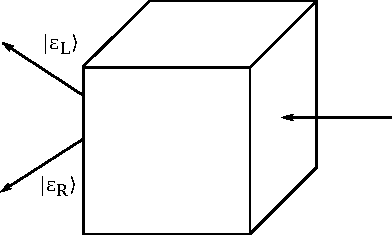
\includegraphics{038ZirkularPolPhotonen}\end{center}

\begin{align}
& \mathrm{linksh"andiges \ Photon:} &  \ket {\varepsilon_L } & = \frac1{\sqrt2} \ket{\varepsilon_x} + \frac i {\sqrt2} \ket{\varepsilon_y} &  &\\
& \mathrm{rechtsh"andiges \ Photon:} & \ket {\varepsilon_R } & = \frac1{\sqrt2} \ket{\varepsilon_x} - \frac i {\sqrt2} \ket{\varepsilon_y} 
\end{align}
$\ket {\varepsilon_L}$ und $\ket{\varepsilon_R}$ stehen orthogonal:
\begin{align}
\begin{split}
\braket{ \varepsilon_R | \varepsilon_L} & = \frac12 \braket{ \varepsilon_x + i \varepsilon_y | \varepsilon_x + i \varepsilon_y } \\
& = \frac12 \braket{ \varepsilon_x | \varepsilon_x } + \frac{i^2}2 \braket{\eps_y | \eps_y} \\
& = 0 
\end{split}
\end{align}
Operatoren: 
\begin{align}
\left.
\begin{array}{l}
P_L = \ket{ \eps_L} \bra{ \eps_L} \\
P_R = \ket{ \eps_R} \bra {\eps_R} 
\end{array}
\right\}
\mathrm{ misst } \left\{
\begin{array}{l}
\mathrm{links-polarisierte}\\
\mathrm{rechts-polarisierte}
\end{array}
\right\} 
\mathrm{ Polarisation \ \ldots}
\end{align}
\ldots bzw. pr"apariert links-/rechtspolarisierte zirkulare Photonen aus einem unpolarisierten Lichtstrahl.

Basiswechsel:

\begin{align}
\begin{split}
P_L = \ket{\eps_L} \bra{\eps_L} & = \frac 12 \left( \ket {\eps_x } + i \ket{ \eps_y} \right) \left( \bra{\eps_x} - i \bra{\eps_y} \right) \\
& = \frac12 P_x + \frac12 P_y + \frac i 2 \ket {\eps_y}\bra{\eps_x} - \frac i 2 \ket{ \eps_x } \bra {\eps_y}
\end{split}
\end{align}
$\Longrightarrow$ Matrixdarstellung bzgl $\set{ \ket{ \eps_x}, \ket{ \eps_y}}$ ist gegeben durch 
\begin{align}
p_L & = \frac12 \begin{pmatrix} 1 & -i \\ i & 1 \end{pmatrix} \quad \mathrm{ links-zirkularer \ Polarisationsfilter}
\end{align}
Es gilt $P_R = \frac12 P_x + \frac12 P_y - \frac i2 \ket{\eps_y}  \bra{ \eps_x} + \frac i2 \ket{ \eps_x} \bra{ \eps_y}$
\begin{align}
\Longrightarrow p_r = p_l^* = \frac12 \begin{pmatrix} 1 & i \\ -i & 1 \end{pmatrix}
\end{align}

\emph{Messung der zirkluaren Polarisation:}
\begin{center}
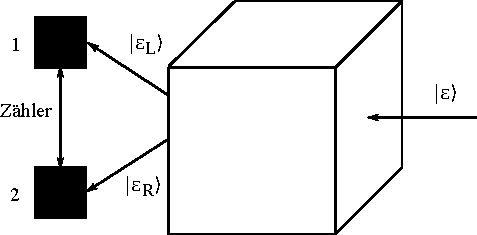
\includegraphics{044MessungZirkPol}
\end{center}
\begin{1aufz}
\item $\ket \eps = \ket{\eps_L}$:
\begin{align*}
\braket{ \eps_L | P_L | \eps_L } & = \braket{\eps_L | \eps_L}\braket{\eps_L | \eps_L} = 1, \\
\braket{ \eps_L | P_R | \eps_L } & = \braket{\eps_L | \eps_R}\braket{\eps_R | \eps_L} = 0, \
\end{align*}
d.h. Z"ahler 1 klickt immer, 2 nie. Das kann man auch "uber die Matrixdarstellung der Operatoren berechnen:
\begin{align*}
\braket{ \eps_L | P_L | \eps_L } & = \frac1{\sqrt2} (1, -i) \frac12 \begin{pmatrix} 1 & -i \\ i & 1 \end{pmatrix} \frac1{\sqrt2} \begin{pmatrix} 1 \\ i \end{pmatrix} \\
& = \frac14 (1, -i) \begin{pmatrix} 2 \\ 2i \end{pmatrix} = 1, \\
\braket{ \eps_L | P_R | \eps_L } & = \frac1{\sqrt2} (1, -i) \frac12 \underbrace{\begin{pmatrix} 1 & i \\ -i & 1 \end{pmatrix} \frac1{\sqrt2} \begin{pmatrix} 1 \\ i \end{pmatrix}}_{=0} = 0 
\end{align*}
Au"serdem gilt f"ur die Unsch"arfe
$$\braket{ \eps_L | (\Delta P_{L,R})^2 | \eps_L } = 0. $$
\item $\ket \eps = \ket { \eps_\phi}$, Basis $\set{ \ket{\eps_x}, \ket{\eps_y}}$:
\begin{align}
\begin{split}
\braket{ \eps_\phi | P_L | \eps_\phi } & = (\cos \phi, \sin \phi) \frac12 \begin{pmatrix} 1 & -i \\ i & 1 \end{pmatrix} \begin{pmatrix} \cos \phi \\ \sin \phi \end{pmatrix} \\
& = (\cos \phi, \sin \phi) \frac 12 \begin{pmatrix} e^{-i\phi} \\ i e^{i\phi} \end{pmatrix} \\
& = \frac 12 e^{-i \phi} \underbrace{ (\cos \phi , \sin \phi) \begin{pmatrix} 1 \\ i \end{pmatrix}}_{= e^{i\phi}} = \frac12
\end{split}
\end{align}
Ebenso 
\begin{align}
\braket { \eps_\phi | P_R | \eps_\phi } = \frac12
\end{align}
$\Longrightarrow$ Jeder Z"ahler spricht in $50 \%$ der F"alle an.

Unsch"arfe:
\begin{align}
\begin{split}
\braket{ \eps_\phi | (\Delta P_{L,R})^2 | \eps_\phi } & = \braket {\eps_\phi | P_{L,R}^2 | \eps_\phi} - \braket{ \eps_\phi | P_{L,R} | \eps_\phi }^2 = \frac14 \\
\Delta P_{L,R}(\eps_\phi) & = \sqrt { \frac 14} = \frac12
\end{split}
\end{align}
\end{1aufz}

\subsubsection*{Kopenhagener Interpretation des Messprozesses}
Messungen ver"andern das physikalische Objekt, das der Messung unterzogen wird. Hat die Messung der Observablen $A$ den Wert $\lambda$ ergeben, so befindet sich das Objekt \emph{nach} der Messung in einem Eigenzustand von $A$ mit Eigenwert $\lambda$ ("`spontane Zustandsreduktion"')

Erwartungswerte selbstadjungierter Operatoren $A$ sind reell:
\begin{align} \braket{ \psi | A | \psi}^* = \braket{ \psi | A^\dagger | \psi} = \braket{ \psi | A | \psi}
\end{align}
Kommutator, Anti-kommutator:
\begin{align}
[A,B] & := AB - BA \\
\{ A,B \} & := AB + BA
\end{align}
Seien $A$ und $B$ selbstadjungiert $(A = A^\dagger, B = B ^\dagger)$. Dann gilt
\begin{align}
[A,B]^\dagger & = - [A,B], \\
\{ A, B \}^\dagger & = \{ A, B \}
\end{align}
Operatoren mit (52) nennt man antiselbstadjungiert.

Betrachte Zustand $\ket \psi$ mit $\braket A = \braket { \psi | A | \psi }$ und $\braket {\psi |\psi }=1$ und die "`Verschiebungen"'
\begin{align}
\begin{split}
\overline A & := A - \braket A \\
\overline B & := B - \braket B 
\end{split}
\end{align}
Herleitung der Unsch"arferelation durch schwarzsche Ungleichung (23):
\begin{align}
\left\Vert \ket { \overline A \psi } \right\Vert \cdot \left\Vert \ket { \overline B \psi }  \right\Vert & \geq \left\vert \braket { \overline A \psi | \overline B \psi } \right\vert \notag\\
& = \left\vert \braket{ \psi | \overline A \overline B | \psi } \right \vert &&  \mathrm{da \ } \overline{ A ^\dagger} = \overline A \notag\\
&  = \frac12 \Big\vert \underbrace{ \braket{ \psi | [\overline A, \overline B ] | \psi}}_{\mathrm{imagin"ar} \Leftarrow \mathrm{(49)}} + \underbrace{\braket { \psi | \{ \overline A, \overline B \} | \psi }}_{\mathrm{reell} \Leftarrow \mathrm{(49)}} \Big\vert \notag\\
& \geq \frac12 \left\vert \braket{\psi | [\overline A, \overline B] | \psi} \right\vert && \mathrm{da \ } \vert z \vert \geq \vert \Im z \vert \notag\\
& = \frac12 \left\vert \braket { \psi | [A,B] | \psi } \right\vert
\end{align}
Unsch"arfe:
$$(\Delta A)^2 = \braket{ \psi | (A - \braket A )^2 | \psi } = \braket{ \overline A \psi | \overline A \psi } = \Vert \ket { \overline A \psi } \Vert^2$$
Mit (55) folgt:
\begin{align} \Delta A \cdot \Delta B \geq \frac12 \vert \braket{ \psi | [A,B] | \psi } \vert \quad \mathrm{Unsch"arferelation} \end{align}
Gilt $[A,B] = 0$, so nennt man $A$ und $B$ kommensurabel (=gemeinsam messbar) oder kompatibel. Es gibt dann eine Basis aus gemeinsamen Eigenkets $\ket { \alpha_i \beta_j }, \ \alpha_i, \beta_i \in \RR$ mit
\begin{align*}
A \ket{ \alpha_i \beta_j } & = \alpha_i \ket{ \alpha_i \beta_j } \\
B \ket{ \alpha_i \beta_j } & = \beta_j \ket{ \alpha_i \beta_j}
\end{align*}
F"ur diese Zust"ande ist $\Delta A = \Delta B = 0$. 

Die Eigenwerte $\alpha_i, \beta_j$ nennt man auch Quantenzahlen von $\ket{ \alpha_i \beta_j}$ zu $A$ und $B$.

\subsubsection*{Stern-Gerlach-Versuch}

1922; I.Stern, W. Gerlach: Silber-Atome: paramagnetisch mit magnetischem Moment $\vv \mu$.
\begin{center}
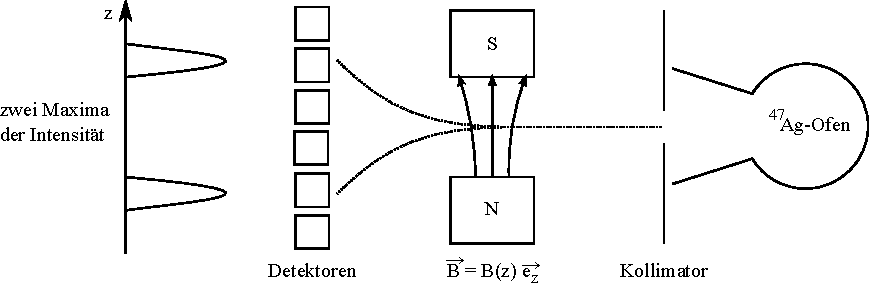
\includegraphics{056SternGerlach}
\end{center}
klassisch:
\begin{align*}
\tag{pot. Energie}  V & = - \vv \mu \vv B\\
\tag{Kraft}  \vv F & = - \nabla V \\
\tag{Kraftkomponente in $z$-Richtung} F_z & = \mu_z \frac {\partial B}{\partial z}
\end{align*}
Atome k"onnen mit jedem Winkel nach oben oder unten abgelenkt werden.

1925: Goudsmit und Uhlenbeck entdeckten den Elektronenspin (=Eigendrehimpuls)
\begin{align}
\vv \mu  = \frac{e}{mc} \vv s, \quad e>0
\end{align}
Silberatom $^{47}Ag$: $\vv \mu$ aus dem 47. $e^-$ (in 5s-Schale).

Schematisch:
\begin{center}
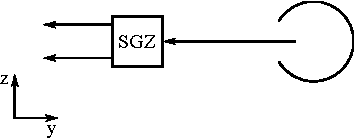
\includegraphics{057SGZ1}
\end{center}

Zwei SGZ hintereinander:
\begin{aaufz}
\item $S_z = \frac \hbar 2$:
\begin{center}
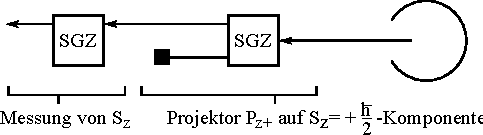
\includegraphics{057SGZ2}
\end{center}
Elektron mit $S_z = \frac \hbar 2$
\begin{align*}
\left. \begin{array}{l} P_{z^+} \\ P_{z^-} \end{array} \right\} \ket{ S_{z^+} } & = \begin{cases} \ket{S_{z^+}} \\ 0 \end{cases} \\
\braket{ S_{z^-} | S_{z^+} } & = 0
\end{align*}

Spin-Operator:
\begin{align}
\begin{split}
S_z \ket{ S_{z^+}} & = \frac \hbar 2 \ket{ S_{z^+}} \\
S_z \ket{S_{z^-}} & = - \frac \hbar 2 \ket{S_{z^-}}
\end{split}
\end{align}
Erwartungswert und Unsch"arfe:
\begin{align}
\braket{ S_z }& = \braket{ S_{z^+} | S_z | S_{z^+}} = \frac \hbar 2 \\
(\Delta S_z)^2 & = \braket { S_{z^+}  | S_z^2 - \frac {\hbar^2}4 | S_{z^+}} = 0 \notag
\end{align}
\item \
\begin{center}
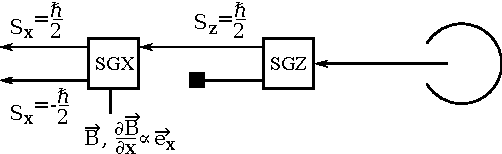
\includegraphics{059SGXSGZ}
\end{center}
$$\ket {S_x+} = \frac \alpha {\sqrt2} \ket{S_{z^+}} + \frac \beta {\sqrt2} \ket{S_{z^-}}$$
$\braket{ S_{x^+} | S_{x^+}} = 1, \ \vert \alpha \vert ^2 + \vert \beta \vert ^2 = 2$ $\leadsto$ gleich gro"se Komponenten $\vert \alpha \vert = \vert \beta \vert = 1$

Allgemein: $\ket \psi$ und $e ^{i \phi} \ket \psi$ beschreiben denselben physikalischen Zustand, denn f"ur alle $A$ gilt:
$$\braket{ \psi | A  | \psi} = \braket{ e^{i \phi} \psi | A | e^{i \phi} \psi }$$
$\leadsto$ o.B.d.A. w"ahle Phasen von $\ket {S_{z^+}}$ und $\ket{ S_{z^-}}$ so, dass $\alpha = \beta = 1$ ist:
\begin{align}
\begin{split}
\ket{ S_{x^+}} & = \frac1{\sqrt2} \ket{S_{z^+}} + \frac1{\sqrt2} \ket{S_{z^-}} \\
\ket{ S_{x^-}} & = -\frac1{\sqrt2} \ket{ S_{z^+}} + \frac1{\sqrt2} \ket{S_{z^-}}
\end{split}
\end{align}
Projektoren:
\begin{align}
\begin{split}
P_{x^\pm} & = \ket{S_{x^\pm}} \bra{S_{x^\pm}} \\
& = \frac12  \ket{ S_{z^+} } \bra{S_{s^+}} \pm \frac 12 \ket {S_{z^+}} \bra{ S_{z^-}} \pm \frac12 \ket{S_{z^-}} \bra{S_{z^+}} + \frac12 \ket{S_{z^-}} \bra{S_{z^-}} 
\end{split} \\
\Longrightarrow p_{x^\pm} = \frac12\begin{pmatrix} 1 & \pm1 \\ \pm 1 & 1 \end{pmatrix}
\end{align}
\emph{Spin-Operator}:
\begin{align} S_x \ket S_{x^\pm} & = \pm \frac \hbar 2 \ket{S_{x^+}} \end{align}
Darstellung bzgl. $\set{ \ket{ S_{z^+}}, \ket{ S_{z^-}}}$: (Invertiere (60))
\begin{align}
\begin{split}
\ket{ S_{z^+}} & = \frac1 {\sqrt2} \left[ \ket{ S_{x^+} }- \ket{ S_{x^-}} \right] \\
\ket{ S_{z^-}} & = \frac1 {\sqrt2} \left[ \ket{ S_{x^+} }+ \ket{ S_{x^-}} \right] 
\end{split}
\end{align}
Es gilt:
\begin{align*}
\braket{ S_{z^+} | S_x | S_{z^+}} & = \frac12 \left[ \braket{S_{x^+} | S_x | S_{x^+} } - \braket{ S_{x^-} | S_x | S_{x^+}} - \braket{ S_{x^+} | S_x | S_{x^-}} + \braket{ S_{x^-} | S_x | S_{x^-}} \right]  \\ 
& = \frac12 \left[ \frac \hbar 2 - \frac \hbar 2 \right] = 0
\end{align*}
Ebenso $\braket{ S_{z^-} | S_x | S_{z^-} } = 0$.

$\leadsto$ genau gleich viele $^{47}$Ag-Atome mit $S_x = \frac \hbar 2$ und $S_x = - \frac \hbar 2$ beobachtet.
\begin{align}
\braket{ S_{z^{\pm}} | S_x | S_{z^\mp}} & = \frac12 \left( \bra{ S_{x^+}} \mp \bra{ S_{x^-}} \right) S_x \left( \bra{ S_{x^+}} \pm \bra {S_{x^-}} \right) \notag \\
& = \frac12 \left[ \frac \hbar2 - \left( \frac \hbar2 \right) \right] ) = \frac \hbar 2 \\
\Longrightarrow s_x & = \frac \hbar 2 \begin{pmatrix} 0 & 1 \\ 1 & 0 \end{pmatrix} 
\end{align}
(65) entspricht
$$\braket{ S_{z^+} | S_x | S_{z^-}} = (1, 0) \frac\hbar2 \begin{pmatrix} 0 & 1 \\ 1 & 0 \end{pmatrix} \begin{pmatrix} 0 \\1 \end{pmatrix} = \frac \hbar 2.$$
\item Nach SGX nochmal SGZ $\leadsto$ $S_z = \frac\hbar2$ und $S_z = - \frac\hbar2$.

Check:
$$ \ket \psi = P_{x^+} \ket{ S_{z^+}} = \ket {S_{x^+}} \braket{ S_{x^+} | S_{z^+}} \stackrel{(61)}= \frac12 \ket{ S_{z^+}} + \frac12 \ket{ S_{z^-}} = \frac1{\sqrt 2} \ket{S_{x^+}}$$

Nun SGY (Apparatur drehen): $x$-Achse und $y$-Achse sind gleichberechtigt. Also:
\begin{align}
\begin{split}
\ket{S_{y	^+}} & = \frac \alpha {\sqrt2} \ket{ S_{z^+}} + \frac \beta {\sqrt2} \ket{ S_{z^-}} \\
\ket{S_{y^-}} & = \frac \alpha {\sqrt2} \ket{ S_{z^+}} - \frac \beta {\sqrt2} \ket{ S_{z^-}}
\end{split}
\end{align}
mit $\vert \alpha \vert = \vert \beta \vert = 1$, $\braket{ S_{y^\pm} | S_z | S_{y^\pm}} = 0$, $\braket{ S_{y^+} | S_{y^-}} = \frac12 \left[ \vert \alpha \vert^2 - \vert \beta \vert^2 \right] = 0$. Weiter:
\begin{align}
\begin{split}
0=\braket{   S_{y^\pm} | S_x | S_{y^\pm}} & =
\frac12 (\alpha^*, \pm \beta^*) \frac \hbar 2 \begin{pmatrix} 0 & 1 \\ 1 & 0 \end{pmatrix} \begin{pmatrix} \alpha \\ \pm \beta \end{pmatrix} \\
& = \pm \frac \hbar 4 (\alpha^* \beta + \beta^* \alpha) \\
& = \pm \frac \hbar 2 \Re (\alpha^* \beta)
\end{split}
\end{align}
Zyklische Vertauschung $(x,y,z) \rightarrow (z,x,y)$:
\begin{align}
\begin{split}
\braket{ S_{y^\pm} | S_x | S_{y^\mp}} & = \braket{ S_{x^\pm} | S_z | S_{x^\mp}} \\
& \stackrel{(60)}= \frac12 \left[ \mp \frac \hbar 2 \mp \frac \hbar 2 \right] = \mp \frac \hbar 2
\end{split}
\end{align}
Andererseits mit (67):
\begin{align}
\begin{split}
\braket{ S_{y^\pm} | S_x | S_{y^\mp}} & = \frac12 (\alpha^*, \pm \beta^*) \frac \hbar 2 \begin{pmatrix} 0 & 1 \\ 1 & 0 \end{pmatrix} \begin{pmatrix} \alpha \\ \mp \beta \end{pmatrix} \\
& = \pm \frac \hbar 4 (- \alpha^* \beta + \beta^* \alpha) = \mp \frac \hbar 2 \Im(\alpha^* \beta)
\end{split}
\end{align}
(68)-(70) bedeuten:
$$\Re(\alpha^* \beta) = 0, \quad \Im(\alpha^* \beta) = 1.$$
L"osung z.B.: $\alpha = 1, \beta = i$. Also:
\begin{align}
\ket{ S_{y^\pm}} = \frac1{\sqrt2} \ket{ S_{z^+} } \pm \frac i{\sqrt2} \ket{ S_{z^-}}
\end{align}
Inverse:
\begin{align}
\begin{split}
\ket{ S_{z+}} & = \frac1{\sqrt2} \left( \ket{S_{y^+}} + \ket{ S_{y^-}} \right) \\
\ket{ S_{z-}} & = \frac i{\sqrt2} \left( - \ket{S_{y^+}} + \ket{ S_{y^-}} \right) \\
\end{split}
\end{align}
Matrixdarstellung:
\begin{align}
s_y & = \frac \hbar 2 \begin{pmatrix} 0 & -i \\ i & 0 \end{pmatrix}
\end{align}
\end{aaufz}
\subsubsection*{Pauli-Matrizen:}
\begin{align}
\begin{split}
\sigma_1 = \sigma_x & = \begin{pmatrix} 0 & 1 \\ 1& 0 \end{pmatrix} \\
\sigma_2 = \sigma_y & = \begin{pmatrix} 0 & -i \\ i & 0 \end{pmatrix} \\
\sigma_3 = \sigma_z & = \begin{pmatrix} 1 & 0 \\ 0& -1 \end{pmatrix}
\end{split}
\end{align}
Spin-Operatoren:
\begin{align}
s_j = \frac \hbar 2 \sigma_j
\end{align}
\emph{Eigenschaften der Pauli-Matrizen}: (siehe Aufgabe 6)
\begin{align}
\begin{split}
\sigma_j \sigma_k & = \delta_{jk} \dOne + \sum_{l=1}^3 i \eps_{jkl} \sigma_l \\
[\sigma_j, \sigma_k] & = 2i \sum_{l=1}^3 \eps_{jkl} \sigma_l
\end{split}
\end{align}
wobei $\eps_{jkl}$ das Levi-Civita-Symbol ist
\begin{align}
\sigma_j &  = \sigma_j^\dagger &  \tr \sigma_j & = 0
\end{align}
Jede hermitesche $2 \times 2$-Matrix $M$ l"asst sich schreiben als
\begin{align}
M & = a_0 \dOne + \sum_{l=1}^3 a_l \sigma_l
\end{align}
Aus (77) folgt
\begin{align}
a_0 = \frac12 \tr M, 
\end{align}
da $\tr \dOne = 2$. Aus (76) folgt:
\begin{align}
\tr [ M \sigma_k] & = \sum_{l=1}^3 a_l \tr [\sigma_l \sigma_k]  = \sum_{l=1}^3 a_l \delta_{lk} \tr \dOne \notag \\
\Longrightarrow a_l & = \frac12 \tr[M, \sigma_l]
\end{align}
(75) / (76) implizieren die Vertauschungsrelationen f"ur die Spinoperatoren:
\begin{align}
[S_j, S_k] & = i\hbar \sum_{l=1}^3 \eps_{jkl} S_l
\end{align}
Wegen $[S_j, S_k] \neq 0$ f"ur $j \neq k$ sind verschiedene Spinkomponenten inkommensurabel. Wegen (siehe (76)) $\sigma_1^2 = \sigma^2_2 = \sigma_3^2 = \dOne$ ist jedoch
\begin{align}
\vv S^2 & = S_x^2 + S_y^2 + S_z^2 = \frac34 \hbar^2 \dOne
\end{align}
Damit ist 
\begin{align}
[\vv S^2, S_j ] = 0, \ j = 1,2,3
\end{align}
D.h. der Gesamtspin $\vv S^2$ "andert sich durch Messung von $S_x, S_y$ und $S_z$ nicht.

\emph{Seltsame Analogie}:

\begin{tabular}{r l | l l}
& Elektron & Photon \\
\hline
(58) & $\uparrow \ \ket {S_{z^+}}$ & $\ket{ \eps_x} \ \vdots$ & \multirow{3}{*}{ \begin{turn}{90}
$\underbrace{\hspace{3.5em}}_{\begin{turn}{270}(5)\end{turn}}$
\end{turn}} \\
(58) & $\downarrow \ \ket{ S_{z^-}}$ & $\ket{ \eps_y} \ \cdots$ \\
(60) &  $\ket{ S_{x^\pm}} = \frac1{\sqrt2} \left[ \pm \ket{S_{z^+}} + \ket{S_{z^-}} \right]$ & $\ket{\eps_{\phi = \frac\pi4}}$, $\ket{\eps_{\phi = \frac{3\pi}4}}$ \\
 & $\ket{S_{y^\pm}} = \frac1{\sqrt2} \left[ \ket{S_{z^+}} \pm i \ket{S_{z^-}} \right]$ & $\ket{\eps_{L,R}}$ & (39)/(40)
\end{tabular}

"Ubliche Schreibweise:
\begin{align}
\begin{split}
\ket{S_{z^+}} & = \ket{ \uparrow } \quad \mathrm{spin \ up} \\
\ket{S_{z^-}} & = \ket \downarrow \quad \mathrm{spin \ down}
\end{split}
\end{align}
Basiswechsel: ($U^\dagger U = \dOne$)
\begin{align}
\begin{split}
\ket{ e_j'} = \ket{ U e_j}, \quad j=1, \ldots, N
\end{split}
\end{align}
Sei $A$ ein selbstadjungierter Operator mit
\begin{align}
A \ket{ e_j} = \lambda_j \ket{ e_j }
\end{align}
Welcher Operator entspricht $A$ in der Basis $\set{ \ket{e_j}}$?
\begin{align*}
\mathrm{(86)} \Longrightarrow U A \underbrace{ U^\dagger U}_{= \dOne} \ket{e_j} & = U \lambda_j \ket{ e_j} \\
\Longrightarrow \ UAU^\dagger \ket{e_j'} & = \lambda_j \ket{e_j'} \\
\Longrightarrow \ A' \ket{ e_j'} & = \lambda_j \ket{ e_j'}
\end{align*}
mit
\begin{align}
A' = UAU^\dagger
\end{align}
Erf"ullen zwei Operatoren $A$ und $A'$ die Gleichung (87), so hei"sen sie unit"ar "aquivalent. I.d.Fall beschreiben sie die selbe Physik, sie haben insbesondere das selbe Spektrum $\set{ \lambda_j }$.

\emph{Beispiel}: $U S_x U^\dagger = S_z$.

Matrixdarstellung von $U$ bzgl. $\set{ \ket \uparrow, \ket \downarrow}$:
$$U = \frac1{\sqrt2} \begin{pmatrix} 1 & 1 \\ i & -i \end{pmatrix}$$
$\Longrightarrow$ $S_z$ und $S_x$ sind physikalisch "aquivalent (EW: $-\frac \hbar 2, \frac \hbar 2$)

Basisunabh"anig: Spur eines Operators $A$:
\begin{align}
\tr A := \sum_{j=1}^N \braket {e_j | A | e_j }
\end{align}
Beweis der Basisunabh"anigkeit: Es gilt die Vollst"andigkeitsrelation: $\sum_{k=1}^N \ket{e_k'} \bra{e_k'} = 1$.
\begin{align*}
\tr A & = \sum_{j,k,l =1}^N \braket{ e_j | e_k'} \braket{ e_k' | A | e_l'} \braket{e_l' | e_j} \\
& = \sum_{j,k,l=1} \braket{ e_k' | A | e_l' } \braket{ e_l' | e_j} \braket{e_j | e_k'} \\
& = \sum_{k,l=1}^N \braket{ e_k' | A | e_l'} \braket{ e_l' | e_k'} \\
& = \sum_{k=1}^N \braket{ e_k' | A | e_k'}
\end{align*} 
Es ist also die Spur von $A$ die Summe seiner Eigenwerte:
\begin{align}
\tr A & = \sum_{j=1}^N \lambda_j.
\end{align}
Ebenso basisunabh"angig:
\begin{align}
\tr A^n = \sum_{j=1}^N \lambda_j^n, \quad n \in \ZZ
\end{align}

\subsection{Ort, Impuls, Energie}
de Broglie: Elektronen verhalten sich wie Wellen, wobei $\vv p = \hbar \vv k$.

Ket f"ur Elektron mit Impuls $\vv p$:
\begin{align}
\ket{\vv p } & \sim e^{i \vv k \vv x} = e^{i \frac{\vv p \vv x}{\hbar}} \quad \mathrm{(ebene Welle)}
\end{align}
Eigenwertgleichung:
\begin{align}
P_j \ket { \vv p} & = p_j \ket{\vv p}, \quad (\vv p = (p_1, p_2, p_3))
\end{align}
Idee: $P_j e^{i \frac{ \vv p \vv x}{\hbar}} = p_j e^{i \frac{ \vv p \vv x }{\hbar}}$ ist erf"ullt, mit der folgenden Definition:
\begin{align}
P_j = -i\hbar \frac{\partial}{\partial x_j}
\end{align}
$P_j$ ist ein Differentialoperator. $P_j$ bildet von einem Funktionenraum in einen (evlt. anderen) Funktionenraum ab. Funktionenr"aume sind Vektorr"aume von Funktionenen $f: x \mapsto f(x)$.

\subsubsection*{(Standard-)Beispiele}
\begin{1aufz}
\item $C[a,b] = $ Menge der auf $[a,b]$ stetigen Funktionen $f: x \in [a,b] \mapsto f(x)$ \\
$C[\RR^n] = $ Menge der auf dem $\RR^n$ stetigen Funktionen, allgemeiner: \\
$C[T] = $ Menge der auf $T \subseteq \RR^n$ stetigen Funktionen

Klar: Mit $f,g$ ist auch $\alpha f + \beta g$ mit $\alpha, \beta \in \CC$ stetig $\Longrightarrow C[\ldots]$ ist Vektorraum

\item $C^n[T] = $ Menge der $n$-mal stetig-differenzierbaren Funktionen $f: x \in T \mapsto f(x)$ \\
$C^\infty[T] = $ Menge der $\infty$-oft stetig diff'baren Funktionen \ldots
\item Schwartz-Raum: umfasst Funktionen die selbst und deren Ableitung f"ur $\vert x \vert \rightarrow \infty$ schneller abfallen als jede Potenz
$$\mathcal S = \mathcal S [\RR] = \left\{ f \in C^\infty[\RR]: \ \sup_{x \in \RR} \left\vert x^p \frac{\mathrm{d}^kf}{\mathrm d x^k } \right\vert < \infty \ \forall p,k \in \NN_0 \right\} $$
Bemerkung: $x \mapsto e^{-\alpha x^2} \in \mathcal S$
$$\mathcal S [\RR^n] = \left\{ f \in C^\infty[\RR^n]: \ \sup_{x \in \RR^n} \left\vert \vert x \vert^p \frac{\partial^{k_1 \ldots k_n}f}{\partial x_1^{k_1} \ldots \partial x_n^{k_n} } \right\vert < \infty \ \forall p,k_1, \ldots, k_n \in \NN_0 \right\} $$
\item $\mathcal L^2[T] = $ Menge aller Funktionen $f$, f"ur die $\int_T \vert f(x) \vert^2 \dd x$ in $\RR$ existiert  = Vektorraum der \emph{quadratisch integrablen Funktionen}
\end{1aufz}
Es gelten:
\begin{itemize}
\item $C^\infty[a,b] \subset C^n[a,b] \subset \ldots \subset C[a,b] \subset \mathcal L^2[a,b],$
\item $\mathcal S[\RR^n] \subset C^\infty[\RR^n] \subset  C^n[\RR^n] \subset \ldots \subset C[\RR^n],$
\end{itemize}
aber weder $C[\RR^n] \supset \mathcal L^2[\RR^n]$ noch $C[\RR^n] \subset \mathcal L^2[\RR^n]$.

Skalarprodukt (=Innenprodukt):
\begin{align}
\braket{ f | g} & = \int_T f^*(x) g(x) \dd x
\end{align}
sinnvoll f"ur 1.) bis 3.)

Die Definitheit (13) ist jedoch f"ur $\mathcal L^2[T]$ verletzt, siehe z.B. f"ur $f \in \mathcal L^2[\RR]$:
\begin{align}
f(x) = \begin{cases} 1, & x=0 \\ 0, & \mathrm{sonst} \end{cases}
\end{align}
Es gilt $\Vert f \Vert^2 = \braket{ f | f} = \int_{-\infty}^\infty \vert f(x) \vert^2 \dd x = 0$, aber $f \neq 0$.

\emph{Trick}: $f$ und $g$ hei"sen "aquivalent ($f \sim g$), wenn 
\begin{align}
\Vert f - g \Vert^2 = \int_T \vert f(x) - g(x) \vert^2 \dd x = 0.
\end{align}
Also: Zwei Funktionen $f,g$, die (96) erf"ullen werden identifiziert, sie beschreiben die selbe Physik. Z.B. erf"ullt $f$ aus (95) $f \sim 0 = $ Nullfunktion.
\begin{1aufz}
\setcounter{enumi}{4}
\item F"ur $T \subseteq \RR^n$:
\begin{align}
L^2[T] & = \mathrm{ Menge \ aller \ "Aquivalenzklassen \ bzgl. \ (96) \ in \ } \mathcal L^2[T]
\end{align}
(94) ist ein Skalarprodukt in $\mathcal L^2[T]$.
\end{1aufz}
R"aume auf denen ein Skalarprodukt definiert ist hei"sen \emph{unit"are R"aume} oder \emph{Innenproduktr"aume}.

D.h. die in 1.), 2.), 3.), 5.) behandelten R"aume sind unit"are R"aume.

Es sei $U$ ein unit"arer Raum und $(f_n) = (f_1, f_2, \ldots)$ eine Folge in $V$ (z.B. $f_n(x) = \frac1n \sin(nx)$). $(f_n)$ hei"st \emph{Cauchyfolge}, wenn es f"ur $\eps > 0$ ein $N \in \NN$ gibt, so dass f"ur alle $m,n \geq N$ gilt:
$$\Vert f_m - f_n \Vert < \eps.$$

Naiv: $(f_n)$ konvergiert gegen ein $f$. Problem: $f$ musst nicht unbedingt in $U$ liegen! 

Besitzt jede Cauchyfolge $(f_n)$ einen Grenzwert $f$ in $V$, so hei"st $V$ \emph{vollst"andig}.

Beispiel mit Zahlenfolgen:
$$\underbrace{\left( 1, \frac{14}{10}, \frac{141}{100}, \frac{1414}{1000}, \ldots \right)}_{\subset \QQ} \longrightarrow \sqrt 2 \notin \QQ$$
$\QQ$ ist also nicht vollst"andig, $\RR$ hingegen schon.

Gibt es eine Basis von $U$, die aus h"ochstens abz"ahlbar vielen Basisvektoren besteht, so hei"st $V$ \emph{separabel}.

Ein \emph{vollst"andiger separabler unit"arer Vektorraum} hei"st \emph{Hilbertraum}

Quantenmechanische Zust"ande entsprechen immer Vektoren (=Kets) in einem Hilbertraum

Die drei wichtigsten Hilbertr"aume:
\begin{1aufz}
\item Jeder endlichdimensionale unit"are Vektorraum ist Hilbertraum
\item $L^2[T]$ mit Skalarprodukt (94), siehe (97), $\mathrm{dim \, } L^2 = \infty$
\item quadratisch summierbare Zahlenfolgen:
\begin{align}
l^2  = \{ (a_n): \sum_{n=0}^\infty \vert a_n \vert^2 < \infty \} \mathrm{ \ mit \ } \braket{ (a_n) | (b_n) }   = \sum_{n=0}^\infty a_n^* b_n
\end{align}
Es gilt $\mathrm{dim \,} l^2 = \infty$
\end{1aufz}
Hilbertr"aume gleicher Dimension sind isomorph, insbesondere $L^2[T] \cong l^2$.
$$
\mathrm{QM}: \left\{
\begin{array}{l l}
\mathrm{math. \ Beschreiben \ in \ } L^2: & \mathrm{Wellenmechanik \ (Schr"odinger)} \\
\mathrm{math. \ Beschreiben \ in \ } l^2: & \mathrm{Matrizenmechanik \ (Hei"senberg, Jordan)}
\end{array}
\right.
$$
Basis in $L^2[T] = $ vollst"andiges orthonormiertes Funktionensystem$\set{ f_0(x), f_1(x), \ldots }$, also 
\begin{aaufz}
\item $\displaystyle \braket{ f_j | f_k} = \int_T \dd^nx f_j^*(x) f_k(x) = \delta_{jk}$ \hfill{} (100)
\item Jedes $f \in L^2[T]$ l"asst sich entwickeln als
\setcounter{equation}{100}
\begin{align}
f(x) & = \sum_{n=0}^\infty a_n f_n(x), \quad a_n \in \CC
\end{align}
\end{aaufz}
Nun ist
\begin{align}
\int_T d^n x f_j^*(x) f(x) = \braket{ f_j | } = \sum_{k=0}^\infty a_n \braket{ f_j | f_k } = a_j
\end{align}
und 
\begin{align}
\Vert f \Vert^2 = \braket{ f | f} \stackrel{(101)}= \sum_{k,n=0}^\infty a_k^* a_n \braket{ f_k | f_n} = \sum_{k=0}^\infty \vert a_n \vert^2
\end{align}
Also:
$$f \in L^2[T] \Longleftrightarrow \braket{ f|f} < \infty \Longleftrightarrow \sum_{k=0}^\infty \vert a_n \vert^2 < \infty \Longleftrightarrow (a_n) \in l^2$$
$f \mapsto (a_n)$ ist also ein isometrischer (wegen (103)) Isomorphismus zwischen $L^2[T]$ und $l^2$.

$(a_n)$ ist  der $\infty$-gro"se Koeffizientenvoektor von $f$ bzgl der Basis $\set{ f_n(x) }$

Analog: $g(x) = \sum_{n=0}^\infty b_n f_n(x)$
\begin{align}
\Longrightarrow \braket{f | g} & = \sum_{n=0}^\infty a_n^* b_n
\end{align}

\subsubsection*{Lineare Operatoren im Hilbertraum $\mathcal H$}
Betrachte Operatoren
\begin{align}
A: f \in \underbrace{\mathcal D(A)}_{\mathrm{Def.-Bereich}} \subset \mathcal H \longrightarrow A f \in \mathcal{H} 
\end{align}
z.B. $P_j$ in (93) ist nicht f"ur alle $f \in L^2$ defininiert, $f$ muss fast "uberall diff'bar sein.
$$\braket{g | P_j f} = \int_T \dd^n x g^*(x) P_jf(x) = \int_T \dd^n x g^*(x) \frac \hbar i \frac \partial{\partial x_j} f(x)$$
ist sinnvoll f"ur $f \in \mathcal D(P_j$ und $g \in L^2$

Physikalische Zust"ande $\psi(x) \in L^2$ hei"sen \emph{Wellenfunktionen}.

Erwartungswert einer Messung von $P_j$:
\begin{align}
\braket{ \psi | P_j | \psi} & = \int_T \dd^nx \psi^*(x) \frac{\hbar}{i} \frac \partial {\partial x_j} \psi(x)
\end{align}
Impulsoperator:
\begin{align}
\vv P & = \frac \hbar i \matr{ \frac \partial {\partial x} \\ \frac \partial {\partial y} \\ \frac \partial {\partial z}} = \frac \hbar i \vv \nabla
\end{align}
Ortsoperator:
\begin{align}
\vv X & = \matr{ X_1 \\ X_2 \\ X_3 }, \mathrm{ \ wobei \ }
X_j: \psi(x) \in \mathcal D (X_j) \subset L^2[T] \longmapsto x_j \psi(x) \tag{(108) + (109)}
\end{align}
\setcounter{equation}{109}
$X_j, P_j$ sind linear und es gelten die \emph{Heisenbergschen Vertauschungsrelationen}:
\begin{eqnarray}
& \left[ X_j, P_k \right]  = i\hbar \delta_{jk}, \\
& \left[ X_j, X_k \right]  = 0 = [ P_j, P_k ]
\end{eqnarray}
Nachweis:
\begin{align*}
[ X_j, P_k] \psi(x) &= (X_j P_k - P_k X_j) \psi(x) \\
& = \frac \hbar i \left[ x_j \frac \partial {\partial x_k} \psi(x) - \frac \partial {\partial x_k} (x_j \psi(x)) \right] \\
& = \frac \hbar i \left[ x_j \frac \partial {\partial x_k} \psi(x) - {\left( \frac \partial {\partial x_k} x_j \right)} - x_j \frac \partial {\partial x_k} \psi(x) \right] \\
& = - \frac \hbar i \delta_{jk} \psi(x) = i \hbar \delta_{jk} \psi(x)
\end{align*}
$\Longrightarrow [X_j, P_k] = i \hbar \delta_{jk}$.

Beschreibt man einen physikalischen Zustand durch eine Wellenfunktion $\psi(x)$ mit $\vv P, \vv X$ in (107), (108), so spricht man von der \emph{Ortsdarstellung}. F"ur $\braket{ \psi | \psi} = 1$ ist der Erwartungswert der Ortsmessung
\begin{align}
\begin{split}
\braket{ \psi | \vv X | \psi} & := \matr{  \braket{ \psi |  X_1 | \psi} \\ \braket{ \psi |  X_2 | \psi} \\ \braket{ \psi |  X_3 | \psi} } \\
& = \int_T \dd^nx \psi^*(x) \vv X \psi(x) \\
& = \int_T \dd^n x \vert \psi(x) \vert^2 x \\
& = \mathrm{"`Schwerpunkt"' \ einer \ Dichteverteilung \ } \vert \psi(x) \vert^2
\end{split}
\end{align}
Wahrscheinlichkeit, das $e^-$ im Volumen $V$ zu finden:
\begin{align}
p(V) & = \int_V \dd^nx \vert \psi(x) \vert^2
\end{align}
Der zu $A$ adjungierte Operator $A^\dagger$ ist verm"oge
\begin{align}
\braket{ A^\dagger f | g} = \braket{ f | Ag}, \quad f \in \mathcal D(A^\dagger), g \in \mathcal D(A).
\end{align}
$A$ hei"st hermitesch (oder symmetrisch), wenn 
\begin{align}
\braket{ Af | g} = \braket{ f  | Ag }, \quad f,g \in \mathcal D(A).
\end{align}
D.h. $A = A^\dagger$ auf $\mathcal D(A)$. Gilt (115) und $\mathcal D(A^\dagger) = \mathcal D(A)$, so hei"st $A$ selbstadjungiert, also $A = A^\dagger$. Es kann passieren, dass (115) erf"ullt ist, aber $\mathcal D(A^\dagger) \supset \mathcal D(A)$ und $A^\dagger \neq A$, d.h. (115) ist verletzt f"ur $f \in \mathcal D(A), f \notin \mathcal D(A^\dagger)$. Dann ist $A$ hermitesch aber \emph{nicht} selbstadjungiert.

Impulsoperator in $L^2[\RR]$:
\begin{align*}
\braket{ f | Pg} & = \frac \hbar i \int_{-\infty}^\infty \dd x f^*(x) \frac d {dx} g(x) \\
& \stackrel {PI}= -\hbar i \int_{-\infty}^\infty \dd x \frac{ f^*(x)}{dx} g(x) + \frac \hbar i \underbrace{\left[ f^*(x) g(x) \right]_{-\infty}^\infty}_{=0}
\end{align*}
$\Longrightarrow f$ hermitesch. Wegen $\int_{-\infty}^\infty \dd x (Pf)^*(x) g(x) = \left[ \int_{-\infty}^\infty \dd x g^*(x) Pf(x) \right]$ ist $\mathcal D(P) = \mathcal D(P^\dagger$.

Ebenso: $X$ ist selbstadjungiert in $L^2[\RR]$.

$A$ hei"st \emph{beschr"ankt}, wenn es eine Zahl $\kappa > 0$ gibt, so dass
\begin{align}
\Vert A f \Vert \leq \kappa \Vert f \Vert, \quad f \in \mathcal H
\end{align}
Beispiele
\begin{itemize}
\item $U$ unit"ar $\Longrightarrow \Vert Uf \Vert = \Vert f \Vert \Rightarrow \kappa =$ m"oglich.
\item $X$ und $P$ sind in $L^2[\RR]$ unbeschr"ankt.
\end{itemize}
Das \emph{Spektrum $\sigma$} eines Operators $A$ besteht aus allen $\lambda \in \CC$ f"ur die $A - \lambda \dOne$ keine beschr"ankte Inverse besitzt. F"ur $\lambda \notin \sigma$ ist die \emph{Resolvente}
\begin{align}
R_\lambda(A) = (A - \lambda \dOne)^{-1}
\end{align}
definiert und beschr"ankt.

Jeder Eigenwert geh"ort zu $\sigma$:
$$(A-\lambda \dOne) f = 0 \ \Longrightarrow (A-\lambda \dOne)^{-1} \mathrm{ \ existiert \ nicht}$$
F"ur $A = A^\dagger$ (d.h. selbstadjungiert) gilt:
\begin{1aufz}
\item $\sigma = \sigma_p \cup \sigma_c$ wobei das Punktspektrum bzw. diskretes Spektrum $\sigma_p$ die Menge der Eigenwerte bezeichnet und $\sigma_c$ kontinuierliches Spektrum hei"st.
\item $\sigma$ enth"alt nur relle $\lambda$. F"ur $\Im \lambda \neq 0$ und $\lambda \notin \sigma$ gilt:
$$\Vert R(\lambda) \Vert \leq \frac 1 {\Im \lambda}$$
Dabei ist die Norm $\Vert A \Vert$ eines Operators $A$ die kleinste Zahl $\kappa \geq 0$ mit $\Vert Af \Vert \leq \kappa \Vert f \Vert$
\item Zu $\lambda \in \sigma_c$ kann man beliebig genaue approximative Eigenvektoren finden:
\begin{align}
\mathrm{Zu \ (jedem) \ } \eps>0 \mathrm{ \ gibt \ es \ ein \ } f_\eps \in \mathcal H \mathrm{ \ mit } \Vert (A-\lambda\dOne) f_\eps \Vert < \eps
\end{align}
Beachte:
$$\lim_{\eps \rightarrow 0} \Vert A - \lambda \dOne) f_\eps \Vert = 0 \Longleftrightarrow \lim_{\eps \rightarrow 0} \Vert R_\lambda f_\eps \Vert = \infty$$
\end{1aufz}

\subsubsection*{Veranschaulichung}
\begin{1aufz}
\item Ortsoperator $X$ in $L^2[\RR]$: Es gilt stets
$$ X \psi(x) = x \psi(x) \neq \lambda \psi(x) \quad \mathrm{f"ur \ } \psi \neq 0$$
$\Longrightarrow \sigma_p = \emptyset$.

Inverses von $X - \lambda \dOne$:
$$R_\lambda: \psi(x) \longmapsto \frac 1{x - \lambda} \psi(x)$$
Das ist wohldefiniert f"ur $\lambda \notin \RR$. F"ur $\lambda \in \RR$ betrachte (siehe Aufgabe 8):
\begin{align}
\psi_\eps(x-\lambda) = (\pi \eps^2)^{-\frac14} e^{-\frac{(x -\lambda)^2}{2 \eps^2}} \in L^2[\RR] \quad \mathrm{(Wellenpakete)}
\end{align}

\psset{xunit=10pt}
\psset{yunit=100pt}
\begin{center}
\begin{pspicture}(6,0)(1,1)

\psplot[plotpoints=100]{0}{10}{2.65 x 5 sub 5 x sub mul exp}
\psplot[plotpoints=100]{0}{10}{2.65 x 5 sub 5 x sub mul exp 0.5 min}
\psline{->}(0,0)(10,0)
\psline{->}(0,0)(0,1)
\psline{-}(5,-0.025)(5,0.025)
\uput[d](5,0){$\lambda$}
\uput[u](5,0.5){$\eps$}
\uput[l](0,1){$\psi_\eps(x)$}
\uput[d](10,0){$x$}
\end{pspicture}
\end{center}
und 
$$\Vert R-\lambda \psi_\eps (x_\lambda) \Vert \longrightarrow \infty, \ \eps \longrightarrow 0, \quad \forall \lambda \in \RR.$$
$\Longrightarrow \sigma = \sigma_c = \RR$.

Approximative Eigenfunktionen von $X$:
$$"' X \psi_\eps (x- \lambda) \approx \lambda \psi_\eps (x - \lambda)"',$$
denn
$$ \Vert (X - \lambda \dOne) \psi_\eps(x - \lambda) \Vert^2 = (\pi \eps^2)^{ - \frac12} \int_{-\infty}^\infty \dd x (x - \lambda)^2 e^{- \frac{(x-\lambda)^2}{\eps}} = \frac {\eps^2}2 \longrightarrow 0, \ \eps \longrightarrow 0.$$
Die Wellenpakete $\psi_\eps(x - \lambda)$ sind also approximative EIgenfunktionen von $X$ zu $\lambda \in \RR$.
\item Impulsoperator: $P = \frac \hbar 2 \frac d {dx}$ in $L^2[\RR]$. Betrachte
$$\psi_p(x) = e^{i \frac p \hbar x}:$$
(91), (93) $\Longrightarrow P \psi_p(x) = p \psi_p(x)$, jedoch $\int_{-\infty}^\infty \psi_p^*(x) \psi_p(x) \dd x = \int_{-\infty}^\infty 1 = \infty$, d.h. $\psi_p(x) \notin L^2[\RR]$.

Approximative Eigenfunktionen zu $p \in \RR$: Breite Wellenpakete:
\begin{align}
\begin{split}
\psi_{p, \eps}(x) & = \psi_{\frac1\eps}(x) e^{i \frac p \hbar x} \\
& = e^{i \frac p \hbar x } \frac {\sqrt \eps}{\pi^{1/4}} e^{- \eps^2 \frac{x^2}{2}} \in L^2[\RR], \\
\Vert \psi_{p,\eps} \Vert & = 1
\end{split}
\end{align}
Es gilt:
$$P \psi_{p, \eps}(x) = p \psi_{p, \eps}(x) + \frac \hbar 2 e^{i \frac p \hbar x} \left( \frac {\eps^2} \pi \right)^{1/4} (- \eps^2 x) e^{- \frac {\eps^2 x^2}2} = p \psi_{p,\eps}(x) + \mathcal O( \sqrt \eps \eps^2 )$$
$\Longrightarrow \sigma_c = \RR$
\end{1aufz}
Ein Operator $U$ hei"st unit"ar, wenn er folgende Eigenschaften erf"ullt:
\begin{1aufz}
\item $\displaystyle \mathcal D(U) = \mathcal H$ \hfill{} (121)
\item Der Wertebereich von $U$ ist $\mathcal H$, d.h. zu jedem $f \in \mathcal H$ gibt es ein $g$ mit $Ug = f$ \hfill (122)
\item $\displaystyle \braket{ Uf | Ug } = \braket{ f | g} \ \forall f,g \in \mathcal H$ ("`L"angen- und Winkeltreue"') \hfill (123)
\end{1aufz}
\setcounter{equation}{123}
Zu 3.) ist "aquivalent, dass $\braket{ Uf | Uf} = \braket{ f|f}$ f"ur alle $f \in \mathcal H$ erf"ullt ist.

\emph{Beweis}:
\begin{align*}
\Vert f \Vert^2 + \Vert g \Vert^2 + 2 \Re \braket{ f | g } & = \Vert f + g \Vert^2 \\
& =  \Vert U(f+g) \Vert^2 \\
& =  \Vert Uf \Vert^2 + \Vert Ug \Vert^2 + 2 \Re \braket{ Uf | Ug}
\end{align*}
d.h. $\Re \braket{ f | g } = \Re \braket{ Uf | Ug}$. Mit $\Vert f + ig \Vert$ analog $\Longrightarrow \Im \braket{ f | g } = \Im \braket{ Uf | Ug}$
\hfill $\square$

F"ur einen unit"aren Operator gilt:
$$U^{-1} = U^\dagger$$
und $U^\dagger$ ist auch unit"ar (d.h. (121),(122) sind erf"ullt.).

Stetige lineare Abbildungen $\phi: V \longrightarrow \CC$ hei"sen Linearformen, lineare Funktionale, Kovektoren oder Bras:
\begin{align}
\braket{ \phi | \alpha f + \beta g} = \alpha \braket{ \phi | f} + \beta \braket{ \phi | g}
\end{align}
$\Longrightarrow$ Die Bras bilden einen Vektorraum, den Dualraum $V^*$.

Ist $V$ ein Hilbertraum $\mathcal H$ mit Basis $\set{ \ket{e_1}, \ket{e_2}, \ldots }$, so gibt es eine Basis $\set{ \bra{e_1}, \bra{e_2}, \ldots}$ in $\mathcal H^*$ mit $\braket{ e_j | e_k} = \delta_{jk}$ und $\mathcal H \cong \mathcal H^*$ mit
\begin{align}
\sum_j \alpha_j \ket{e_j} \longleftrightarrow \sum_j \alpha_j^* \ket{ e_j}
\end{align}
F"ur $L^2[\RR]$ bedeutet dies: Jede Linearform $\phi: f \in L^2[\RR] \longmapsto \phi[f] \in \CC$ l"asst sich schreiben als 
\begin{align}
\phi[f] = \braket{ \phi | f} = \int_{-\infty}^\infty \dd x \tilde \phi^*(x) f(x)
\end{align}
mit einem $\tilde \phi \in L^2[\RR]$.

Ist $V$ kein Hilbertraum, so gilt dies nicht:

\emph{Beispiel}: $V = \mathcal S[\RR]$. Betrachte
$$ \delta: f \in \mathcal S[\RR] \longmapsto \delta[f] = f(0)$$
Es gilt $\delta \in \mathcal{S}^*[\RR]$, da die Punktauswertung linear und stetig ist.

Symbolische Schreibweise wie in (126):
$$ \delta[f] = f(0) =: \int_{-\infty}^\infty \dd x \delta(x) f(x), \quad \delta(x) = \delta\mathrm{-Funktion} = \delta\mathrm{-Distribution}$$
Dualraum zu $\mathcal S[\RR]$:
\begin{align*}
\mathcal S^*[\RR] & = \mathrm{Vektorraum \ der \ gem"a"sigten \ Distributionen} \\
& = \mathrm{temperierte \ Distributionen} \\
& = \mathrm{tempered \ distribitions}
\end{align*}
( $\mathcal S^*[\RR], L^2[\RR], \mathcal S [\RR]$ ) ist ein Beispiel f"ur ein Gelfandsches Raumtripel:
\begin{align}
\mathrm{
\setlength{\tabcolsep}{2pt}
\begin{tabular}{r c l}
$\mathcal S^*[\RR]$ & $\supsetneqq L^2 [\RR] \supsetneqq$ & $\mathcal S[\RR]$ \\
Mehr Bras & & weniger Kets
\end{tabular}
}
\end{align}
Vorteil: In $\mathcal S^*[\RR]$ k"onnen wir f"ur $A = A^\dagger$ jedem $\lambda \in \sigma(A)$ eine Eigendistribution finden, z.B $\psi_p(x) = e^{\frac {i p x}{\hbar}} \notin L^2[\RR]$, aber mit der Zuordnung $\psi_p^*(x) \leftrightarrow \bra p$ gilt:
\begin{align}
\bra p P = \bra p p,
\end{align}
au"serdem ist  f"ur alle $f \in \mathcal S[\RR]$
\begin{align}
\braket{ p | f} = \int_{-\infty}^\infty \dd x \, \psi_p^*(x) f(x) = \int_{-\infty}^\infty \dd x \,  e^{- \frac{px}\hbar} f(x)
\end{align}
wohldefiniert und (129) beschreibt eine stetige lineare Abbildung von $\mathcal S[\RR]$ auf $\CC$.

D.h. ebene Wellen sind gem"a"sigte Distributionen.

Flexible Notation:
$$\langle \underbrace{f}_{\mathrm{Bra}\in \mathcal S^*}  | \underbrace{g}_{\mathrm{Ket}\in\mathcal S} \rangle = \langle \underbrace{g}_{\in \mathcal S} | \underbrace{f}_{\in \mathcal S^*} \rangle^*$$

Achtung: F"ur $f,g \in \mathcal S^*[\RR]$ ist $\braket{ f|g}$ nicht immer definiert. Beispiel: $\braket{ \psi_p | \psi_p}  = \int_{-\infty}^\infty \dd x \, 1 = \infty$.

verallgemeinerte Eigenfunktionen (Eigenbras) zu $X$ gesucht:
\begin{align}X \psi_{x_0}(x) = x_0 \psi_{x_0}(x) \quad \mathrm{ mit \ } x_0 \in \RR.
\end{align}
L"osung:
\begin{align}
\psi_{x_0}(x) = \delta(x -x_0) \in \mathcal S^*[\RR]
\end{align}
Auch hier ist $\braket{ \psi_{x_0} | \psi_{x_0}} = \int_{-\infty}^\infty \dd x \, \delta(x-x_0) \delta(x-x_) = \infty$ nicht definiert!

Die verallgemeinerten Eigenfunktionen selbstadjungierter Operatoren $A$ sind vollst"andig. Die Entwicklung nach Eigenvektoren $ \ket{f} = \sum_{\lambda \in \sigma} \ket{\lambda} \braket{ \lambda | f }$ wobei $A \ket{\lambda} = \lambda \ket \lambda$ im endlichdimensionalen Fall liest sich nun (im $\infty$-dimensinalen Fall) wie folgt (f"ur ohne entartete Eigenvektoren):
\begin{align}
\ket f = \sum_{\lambda \in \sigma_p} \ket \lambda \braket{ \lambda | f} + \int_{\sigma_c} \dd \lambda \, \ket \lambda \braket{ \lambda | f}
\end{align}
Ortsoperator:
\begin{align} X \ket \psi = x \ket \psi \end{align}
verallgemeinerte Eigenvektoren: $X \delta(x-x_0) = x_0 \delta(x-x_0)$ bzw. symbolisch $X \ket{x_0} = x_0 \ket{x_0}.$
\begin{align}
\ket \psi = \int_\RR \dd x_0 \, \ket {x_0} \braket{ x_0 | \psi}
\end{align}
entspricht
$$ \psi(x) = \int_{-\infty}^\infty \dd x_0 \, \underbrace{ \delta(x-x_0) }_{\ket{x_0}} \underbrace{\int_{-\infty}^\infty \dd x' \, \delta(x' - x_0) \psi(x')}_{\braket{ x_0 | \psi}} = \psi(x)$$
Impulsoperator:
$$P  N e^{i \frac {px}{\hbar}} = p \underbrace{ N e^{i \frac{px} \hbar}}_{\widehat \, = \ket p}, \quad N    =  \mathrm{ Normierungskonstante}$$
Die Entwicklung nach Eigenvektoren $\ket \psi = \int_{-\infty}^\infty \dd p \, \ket p \braket{ p | \psi}$ bedeutet
\begin{align}
\psi(x) & = \underbrace{ \int_{-\infty}^\infty \dd p \, e^{i \frac {px}\hbar} \vert N \vert^2 }_{\mathrm{inverse \ Fouriertrafo}} \underbrace{ \int_{-\infty}^\infty \dd x' \,  e^{- i \frac{px'} \hbar} \psi(x') }_{\mathrm{Fourier-Trafo}} \quad \mathrm{f"ur \ } \vert N \vert ^2 = \frac 1 {2 \pi \hbar}
\end{align}
Speziell f"ur $\ket \psi = \ket {x_0}$:
\begin{align}
\braket {p | x_0} & = \frac1{\sqrt{2 \pi \hbar}} e^{- i \frac {p x_0}\hbar} \quad \mathrm{"`Ortseigenzustand \ in \ Impulsdarstellung"'}
\end{align}
In (134) mit $\ket \psi = \ket p$
$$ \ket p = \int_\RR \dd x' \, \ket {x'} \braket{ x' | p} \stackrel{(136)}= \int_{-\infty}^\infty \dd x' \, \ket{ x'} \frac1{\sqrt{2\pi\hbar}} e^{i \frac{px'}\hbar}$$
Konsistenzcheck (der Vollst"andigkeit):
\begin{align}
\begin{split}
\frac1{\sqrt{2\pi\hbar}} e^{i \frac{px}\hbar} & = \braket{ x | p } \\
& = \int_{-\infty}^\infty \dd x' \, \braket{ x | x'} \frac1{\sqrt{2 \pi \hbar}} e^{i \frac {px'}\hbar} \\
& = \frac1{\sqrt{2\pi\hbar}} e^{i \frac{px}\hbar} \checkmark
\end{split}
\end{align}
in (137) wurde verwendet:
\begin{align}
\braket{x | x'} = \int_{-\infty}^\infty \dd x'' \, \delta(x - x') \delta(x' - x'') = \delta(x - x')
\end{align}
Normierung der Impulseigenzust"ande:
\begin{align}
\begin{split}
\braket{ p | p'} & = \int_{-\infty}^\infty \frac{ e^{- i \frac{px}\hbar}}{\sqrt{2 \pi \hbar}} \frac{e^{ i \frac{p'x}\hbar}}{\sqrt{2 \pi \hbar}} \\
& = \frac1{\sqrt{2\pi\hbar}} (2 \pi) \delta\left( \frac p \hbar - \frac {p'} \hbar \right) \\
& = \frac 1 \hbar \delta \left( \frac{ p - p'} \hbar \right) \\
& = \delta( p - p')
\end{split}
\end{align}
analog zu (138).

Projektion eines Zustandes $\ket \psi$ auf Ortseigenzustand:
\begin{align}
\braket{ x | \psi} = \int_{-\infty}^\infty \dd x' \, \delta (x - x') \psi(x') = \psi(x) = \mathrm{ Wellenfunktion \ in \ Ortsdarstellung }
\end{align}
Projektion auf Impulseigenzustand:
\begin{align}
\begin{split}
\braket{ p | \psi} & = \int_{-\infty}^\infty \frac1{\sqrt{2\pi\hbar}} e^{-i \frac{px}\hbar} \psi(x) =: \widetilde \psi(p) \\
&  = \mathrm{Impulsdarstellung} \\
& = \mathrm{Fourier-Transformierte \ von \ } \psi(x)
\end{split}
\end{align}
Umkehrfunktion
\begin{align}
\begin{split}
\psi(x) = \braket{ x | \psi } & = \int_{-\infty}^\infty \braket{ x | p'} \underbrace{ \braket{ p' | x}}_{= \widetilde \psi(p')} \dd p' \\
& = \frac1{\sqrt{2 \pi \hbar}} \int_{-\infty}^\infty \dd p' \, e^{i \frac{p'x}\hbar} \widetilde \psi(p')
\end{split}
\end{align}
Ortsoperator in Impulsdarstellung:
\begin{align}
\begin{split}
\braket{ p | X | \psi} & = \int_{-\infty}^\infty \dd p' \, \braket{ p | X | p'}\braket{p' | \psi} \\
& = \int_{-\infty}^\infty \dd p' \, \braket{p | X | p'} \widetilde \psi(p')
\end{split}
\end{align}
Nun ist 
\begin{align}
\begin{split}
\braket{ p | X | p'} & = \int_{-\infty}^\infty \dd x \, \frac{ e^{ - \frac{i p x}\hbar}}{\sqrt{2\pi \hbar}} x \frac{ e^{\frac{ipx}\hbar}}{\sqrt{2 \pi \hbar}} \\
& = \frac1{{2\pi\hbar}} \frac \hbar i \frac \partial {\partial p'} \underbrace{ \int_{-\infty}^\infty \dd x \, e^{-\frac{ipx}\hbar} e^{\frac{ip'x}\hbar}}_{2 \pi \delta(\frac{p - p'}\hbar)} \\
& = \frac \hbar i \frac \partial {\partial p'} \delta(p - p')
\end{split}
\end{align}
Einsetzen in (143):
\begin{align}
\begin{split}
\braket{ p | X | \psi} & \stackrel{\mathrm{P.I.}}= \int_{-\infty}^\infty \delta(p-p') \left( - \frac \hbar i \right) \frac \partial {\partial p'} \widetilde \psi(p') \\
& = - \frac \hbar i \frac \partial {\partial p} \widetilde \psi (p)
\end{split}
\end{align}
Impulsoperator in Impulsdarstellung:
$$ \braket{ p | P | \psi} = p  \braket{ p| \psi} = p \widetilde \psi(p)$$
Zusammenfassung:
\begin{center}
\begin{tabular}{r | c  | c }
& Ortsdarstellung & Impulsdarstellung \\
\hline
Ortsoperator $X$ & $x \psi (x)$ & $\frac \hbar i \frac \partial {\partial p} \widetilde \psi(p)$ \\
Impuloperator $P$ & $\frac \hbar i \frac \partial {\partial x} \psi(x)$ & $p \widetilde \psi(p)$
\end{tabular}
\end{center}

\subsubsection*{Energie}
\begin{center}
\begin{tabular}{l l }
klassische Mechanik: & Hamiltonfunktion $H(x_j, p_k)$ \\
QM: & $H(X_j, P_k)$
\end{tabular}
\end{center}
Teilchen im Potenzial:
\begin{align}
H(\vv X, \vv P) & = \frac{ \vv P^2}{2m} + V(\vv X)
\end{align}
Eigenzust"ande $\ket E$ zum Energieeigenwert $E$
\begin{align}
H(\vv X, \vv P) \ket E & = E \ket E
\end{align}
Energiezust"ande hei"sen auch \emph{station"are Zust"ande}. Die diskreten Eigenwerte $E_n$ (= Elemente von $\sigma_p$, $n=0,1,2, \ldots$) von $H$ ("`Energieniveaus"') entsprechen Bindungszust"anden $\ket {E_n}$, da $\braket{ E_n | E_n} < \infty$. Die uneigentlichen Eigenwerte (= Elemente von $\sigma_c$) von $H$ entsprechen Streuzust"anden $\ket E$, da $\braket{ E | E } = \infty$.

\emph{Ortsdarstellung}: 

(147) lautet in der Ortsdarstellung $\braket{ \vv x | H | E} = E \braket{ \vv x | E}$.
\begin{align}
\int \dd^3 \vv x \, \braket{ \vv x | H | \vv x'} \underbrace{ \braket{\vv x ' | E}}_{\psi_E(\vv x')} & = E \underbrace{ \braket{ \vv x | E}}_{\psi_E(\vv x)}
\end{align}
Es gilt
\begin{align*}
\Braket{ \vv x | H | \vv x'} & = \Braket{ \vv x| \frac{ \vv P^2}{2m} + V( \vv X) | \vv x'} \\
& = \Braket{ \vv x | \frac{ \vv P^2}{2m} | \vv x'} + \underbrace{\Braket{ \vv x | V(\vv X) | \vv x'}}_{V(\vv x) \underbrace{\Braket{ \vv x | \vv x }}_{\delta^{(3)}(\vv x - \vv x')}}
\end{align*}
und
\begin{align}
\begin{split}
\Braket{ \vv x | \frac{ \vv P^2}{2m} | \vv x'} & = \frac1{2m} \int \dd^3 \vv p \, \Braket{ \vv x | \vv P | \vv p }\Braket{ \vv p | \vv P | \vv x'} \\
& = \frac1{2m} \int \dd^3 \vv p \, \vv p^2 \Braket{ \vv x | \vv p }\braket{ \vv p | \vv x}
\end{split}
\end{align}
3D-Version von (137):
\begin{align} 
\Braket{ \vv x | \vv p } = \frac1{(2 \pi \hbar)^{\nicefrac32}} e^{\frac{i \vv p \vv x}{\hbar}}
\end{align}
Einsetzen in (149):
\begin{align}
\begin{split}
\Braket{ \vv x | \frac{ \vv P^2}{2m} | \vv x' } & = \frac1{2m} \frac1{(2\pi \hbar)^{\nicefrac32}} \int \dd^2 \vv p \, \underbrace{ \vv p^2 e^{\frac{ i \vv p ( \vv x  - \vv x')} \hbar}}_{- \hbar^2 \Delta e^{\frac{i \vv p ( \vv x - \vv x')}\hbar}} \\
& \stackrel{ \vv k = \frac{\vv p}{\hbar}}=  - \frac{\hbar^2}{2m} \Delta\underbrace{ \frac1{(2\pi)^3} \int \dd^3 \vv k \, e^{i \vv k ( \vv x - \vv x')}}_{\delta^{(3)}(\vv x - \vv x')}
\end{split}
\end{align}
Einsetzen in (148):
$$\int \dd^3 \vv x' \psi_E(\vv x) \left[ - \frac{\hbar^2}{2m} \Delta \delta^{(3)} (\vv x - \vv x') + V( \vv x) \delta^{(3)} (\vv x - \vv x') \right] = E \psi_E(\vv x)$$
partielle Integration:
\begin{align}
\int \dd^3 \vv x' \, \left[ - \frac{\hbar^2}{2m} \Delta \psi_E( \vv x') + V(\vv x) \psi_E(\vv x') \right] \delta^{(3)}(\vv x - \vv x') & = E \psi_E(\vv x) \ \Longleftrightarrow \notag \\
\left[ -\frac{\hbar^2}{2m} \Delta + V(\vv x) \right] \psi_E(\vv x) & = E \psi_E(\vv x)
\end{align}
(152) hei"st \emph{zeitunabh"angige Schr"odinger-Gleichung}. Ihre L"osungen $\psi_E(\vv x)$ sind Energie-Eigenfunktionen. Salopp:
\begin{align}
H \psi_E(\vv x) & = E \psi_E(\vv x), \quad H = - \frac{\hbar^2}{2m} \Delta + V(\vv x) = \mathrm{Hamilton-Op. \ in \ Ortsdarstellung}
\end{align}
\emph{Impulsdarstellung}:
\begin{align}
\left[ \frac{\vv p^2}{2m} + V(i\hbar \vv \nabla_p) \right] \widetilde \psi (\vv p) = E \widetilde \psi(\vv p) \quad \mathrm{mit \ } \vv \nabla_p = \matr{ \nicefrac \partial {\partial p_x} \\ \nicefrac \partial {\partial p_y} \\ \nicefrac \partial {\partial p_z}}  
\end{align}
praktisch f"ur lineare Potenziale $V(\vv x) = \alpha \vv x$ und f"ur Streuprobleme.

\subsection{Tensorprodukt}

2 Hilbertr"aume $\mathcal H = \left[ \ket{e_1}, \ket{e_2}, \ldots \right]$ und $\mathcal H' = \left[ \ket{e_1'}, \ket{e_2'}, \ldots \right]$.
\begin{align}
\mathrm{Tensorprodukt \ } \mathcal H \otimes \mathcal H' = \left[ \ket{e_j} \otimes \ket{e_k'} \right]
\end{align}
dabei werden die $\ket{e_j} \otimes \ket{e_k'}$ auch oft mit $\ket{e_j} \ket{e_k'}$ oder $\ket{ e_j e_k'}$ bezeichnet.

F"ur $\mathrm{dim} \mathcal H = N, \ \mathrm{dim} \mathcal H' = N'$ ist $\mathrm{dim} \left[ \mathcal H \otimes \mathcal H' \right] = N \cdot N'$. F"ur
$$\ket{\alpha} = \sum_k \alpha_k \ket{e_k} \quad \mathrm{und} \quad \ket{\alpha'} = \sum_l \alpha_l' \ket{e_l'}$$
ist
\begin{align}
\ket \alpha \otimes \ket{ \alpha'} = \sum_{k,l} \alpha_k \alpha_l' \ket{e_k} \otimes \ket{e_l'}
\end{align}
Nicht jedes Element von $\mathcal H \otimes \mathcal H'$ l"asst sich schreiben als $\ket \alpha \otimes \ket{\alpha'}$. Allgemein gibt es f"ur $\ket \lambda \in \mathcal H \otimes \mathcal H'$ Zahlen $\alpha_{kl} \in \CC$, so dass
\begin{align}
\ket \lambda = \sum_{kl} \alpha_{kl} \ket{e_k} \otimes \ket{e_l'}.
\end{align}
Bras:
\begin{align}
\begin{split}
( \bra \beta \otimes \bra{\beta'})(\ket \alpha \otimes \ket{\alpha'}) & = \braket{ \beta | \alpha} \braket{ \beta' | \alpha'} \\
& = \left( \sum_k \beta_k^* \alpha_k \right) \left( \sum_l \beta_l'^* \alpha_l' \right), \quad \mathrm{f"ur \ } \ket \beta = \sum_l \beta_l \ket{e_l}
\end{split}
\end{align}
Zu Operatoren $A$ auf $mathcal H$, $A'$ auf $\mathcal H'$ sind 
$$A \otimes \dOne \quad \mathrm{und} \quad \dOne \otimes A'$$
Operatoren auf $\mathcal H \otimes \mathcal H'$ mit
\begin{align}
\begin{split}
(A \otimes \dOne)( \ket \alpha \otimes \ket{\alpha'}) & = \ket{A \alpha} \otimes \ket{\alpha'} \ \mathrm{und} \\
( \dOne \otimes A')(\ket \alpha \otimes \ket{\alpha'} & = \ket \alpha \otimes \ket{ A' \alpha'}
\end{split}
\end{align}
Salopp schreibt man $A$ (bzw. $A'$) statt $A \otimes \dOne$ (bzw. $\dOne \otimes A'$). 

Insbesondere gilt
\begin{align} [ A, A'] & = 0, \end{align}
denn $A A' \ket \alpha \ket{\alpha'} = \ket{ A \alpha }\ket{ A' \alpha'} = A'A \ket \alpha \ket{\alpha'}$

\emph{Anwendung}: $\mathcal H = [ \ket \uparrow, \ket \downarrow]$ beschreibt Spin-Freiheitsgrad (ist innerer Freiheitsgrad) und $\mathcal H' = L^2[\RR]$ beschreibt "au"sere Freiheitsgrade (z.B. Orts-Wellenfunktion). Beliebiger Zustand $\ket \chi$ in $\mathcal H \otimes \mathcal H'$ f"ur $\mathcal H' = [ \ket{\psi_1}, \ket{\psi_2}, \ldots ]$:
\begin{align}
\begin{split}
\ket \chi & \stackrel{(157)}= \sum_{k=\uparrow, \downarrow} \sum_l \alpha_{kl} \ket k \otimes \ket{\psi_l} \\
& = \sum_l \alpha_{\uparrow l} \ket \uparrow \otimes \ket{\psi_l} + \sum_l \alpha_{\downarrow l} \ket \downarrow \otimes \ket{\psi_l} \\
& = \ket \uparrow \otimes \ket{\psi_\uparrow} + \ket \downarrow \otimes \ket{\psi_\downarrow}
\end{split}
\end{align}
Pauli-Spinor = zwei-komponentige Wellenfunktion
\begin{align}
\matr{ \psi_\uparrow(\vv x) \\ \psi_\downarrow(\vv  x) } & = \matr{( \bra \uparrow \otimes \bra{\vv x}) \ket X \\ ( \bra \downarrow \otimes \bra{ \vv x}) \ket X} \stackrel{(158),(161)}= \matr{ \braket{ \vv x | \psi_\downarrow} \\ \braket{ \vv x | \psi_\downarrow}}
\end{align}
Interpretation: $\int_V \dd^3 \vv x \, \vert \braket{ x | \psi_\uparrow} \vert^2 = $ Wahrscheinlichkeit im Volumen $V$ ein Elektron mit $S_z = \frac \hbar 2$ zu finden.

\subsection{Zeitentwicklung}

\emph{Klassische Mechanik}: Symmetrien $\stackrel{\mathrm{Noether-Thm}}\Longrightarrow$ Erhaltungsgr"o"sen.

z.B. Symmetrie unter Translationen $\vv x \mapsto \vv x + \vv a$ $\Longrightarrow$ Impuls $\vv p$ erhalten ($\frac{\dd \vv p}{\dd t} = 0$).

\emph{QM}: $\frac{\vv p }{\hbar}$ ist Generator der Translationen:
\begin{align}
\mathcal T _{\vv a}= e^{\frac i \hbar \vv a \vv p}; \quad \mathcal T _{\vv a} \psi(\vv x) = \psi(\vv x + \vv a) \ (\mathrm{siehe \ A 7c})
\end{align}
Analogie zwischen klassischer Mechanik und QM:

Symmetrie bzgl. $t \mapsto t + \Delta t \Longrightarrow$ Hamiltonfunktion $H$ ist zeitlich konstant: $\frac { \dd H }{\dd t} = 0$.
\begin{align}
\begin{split}
M(t_0+t, t_0) \psi(\vv x, t_0) & = \psi(\vv x, t_0 + t) \\
\mathrm{bzw. \ } M(t_0 + t, t_0) \ket{ \psi, t_0} & = \ket{ \psi, t_0+t}
\end{split}
\end{align}
mit dem Zeitentwicklungsoperator (= Translationsoerator in der Zeit)
\begin{align}
M(t_0,t, t_0) & = e^{- \frac i \hbar t H} \quad \mathrm{f"ur \ } \frac{d H}{dt} = 0
\end{align}
Differenziell:
\begin{align*}
i \hbar \frac \partial {\partial t} \psi(\vv x, t_0 + t) & \stackrel{(164)}= i \hbar \frac \partial {\partial t} M(t_0+t, t_0) \psi(\vv x, t_0) \\
& = i \hbar \frac \partial {\partial t} e^{-\frac i \hbar t H} \psi( \vv x, t_0) \\
& = H e^{-\frac i \hbar t H} \psi(\vv x, t_0) \\
& = H \psi(\vv x, t_0 + t)
\end{align*}
F"ur $t_0 =0$:
\begin{align}
\begin{split}
i \hbar \frac \partial {\partial t} \psi(\vv x, t) & = H \psi( \vv x, t) \ \mathrm{bzw.} \\
i \hbar \frac \partial {\partial t} \ket{ \psi, t} & = H \ket{ \psi, t}
\end{split}
\end{align}

(166) hei"st \emph{zeitabh"angige Schr"odinger-Gleichung}. F"ur $\frac {dH}{dt} \neq 0$ sind (165) und (166) nicht mehr "aquivalent. (166) stimmt auch f"ur $\frac{dH}{dt} \neq 0$.

Gilt $[ H(t_1), H(t_2) ] = 0$ f"ur alle $t_1, t_2$, so 
\begin{align}
M(t_0+t, t_0) & = e^{-\frac i \hbar \int_{t_0}^{t_0+ t} \dd t' \, H(t')}
\end{align}
Zeitgeordnetes Produkt:
\begin{align}
\begin{split}
T A(t_1) B(t_2) = T B(t_2) A(t_1) & = \theta (t_1 - t_2) A(t_1) B(t_2) + \theta(t_2-t_1) B(t_2) A(t_1) \\
& = \begin{cases} A(t_1) B(t_2), & t_1 > t_2 \\
B(t_2) A(t_1), & t_1 < t_2 \end{cases}
\end{split}
\end{align}
Analog $T A(t_1) B(t_2) C(t_3) = \theta(t_1 - t_2) \theta(t_2 - t_3) A(t_1) B(t_2) C(t_3) + \theta(\ldots) \ldots$
F"ur $t_1 = t_2$ ist $T A(t_1) B(t_2)$ i.a. nur f"ur $A=B$ definiert.


Anwendung:
\begin{align}
& \int\limits_{t_0}^{t_0+t} \dd t_1 \int\limits_{t_0}^{t_0 + t} \dd t_2 \, T H(t_1) H(t_2) = \int\limits_{t_0}^{t_0 + t} \dd t_1   \int\limits_{t_0}^{t_1} \dd t_2 \, H(t_1) H(t_2) +  \int\limits_{t_1}^{t_0+t} \dd t_2 \, H(t_2) H(t_1) \\
& \frac d {dt} (169) = \int\limits_{t_0}^{t_0+t} \dd t_2 \, T H(t_0+t) H(t_2) + \int\limits_{t_0}^{t_0+t} \dd t_1 \, T H(t_1)H(t_0+t)
\end{align}
Regel:
$$ \frac d {dt} \int_a^t \dd t' \int_b^t \dd t'' \, f(t') g(t'') = \int_b^t \dd t'' \, f(t) g(t'') + \int_a^t \dd t' \, f(t') g(t)$$
Daraus folgt:
\begin{align}
\frac d {dt} (169) & = H(t_0 + t) \cdot 2\dot \int_{t_0}^{t_0 + t} \dd t_1 \, H(t_1)
\end{align}
Dabei ist die Zeitordnung trivial wegen $t_0 + t \geq t_1$.

\subsubsection*{zeitgeordnete Exponentialreihe = Dyson-Reihe}
\begin{align}
T \exp \left[ \int_{t_0}^{t_0+t} A(t') \dd t' \right] := 1 + \sum_{k=1}^\infty \frac 1  {R!} \int_{t_0}^{t_0+t} \dd t_1 \ldots \int_{t_0}^{t_0 + t} \dd t_k \, T A(t_1) \ldots A(t_k)
\end{align}
Gilt $[A(t), A(t')] = 0$, so ist $T \exp = \exp$
\begin{align*}
\frac d{dt} T \exp \left[ \int_{t_0}^{t_0+t} A(t') \dd t \right] &=  \sum_{n=1}^\infty \frac1{n!}
\Big[
\begin{aligned}[t]
& \int_{t_0}^{t_0 + t} \dd t_2 \ldots \int_{t_0}^{t_0+t} \dd t_n \,  T A(t_0+t) A(t_2) \ldots A(t_n)  \\
& + \int_{t_0}^{t_0 + t} \dd t_1 \int_{t_0}^{t_0+t} \dd t_3 \ldots \int_{t_0}^{t_0+t} \dd t_n \,  TA(t_1) A(t_0 + t) \ldots A(t_n) \\ & +  \ldots \\
 & + \int_{t_0}^{t_0+t} \dd t_1 \ldots \int_{t_0}^{t_0+t} \dd t_{n-1} \, T A(t_1) \ldots A(t_{n-1}) A(t_0+t) \Big]
\end{aligned}  \\ 
& = A(t_0+t) \sum_{n=1}^\infty \frac1{(n-1)!} \int_{t_0}^{t_0+t}\dd t_1 \ldots \int_{t_0}^{t_0 +t} \dd t_{n-1} \, T A(t_1) \ldots A(t_{n-1})
\end{align*}

Mit $n \rightarrow n +1$ findet man
\begin{align}
\frac d {dt} T \exp \left[ \int_{t_0}^{t_0+t} \dd t' A(t') \right] & = A(t_0 + t) T \exp \left[ \int_{t_0}^{t_0+t} \dd t' A(t') \right]
\end{align}
Sehr praktisch f"ur gekoppelte Differntialgleichung:
\begin{align*}
\dot {c_1} & = A_{11}(t) c_1 + \ldots + A_{1n}(t) c_n \\
\vdots \\
\dot {c_n} & = A_{n1}(t) c_1 + \ldots + A_{nn}(t) c_n, \\
\end{align*}
also $\dot{ \vv c} = A(t) \vv c$. L"osung:
\begin{align}
\vv c(t) = T \exp \left[ \int_{0}^t \dd t' A(t') \right] \vv c(0),
\end{align}
denn $\dot{ \vv c}(t) \stackrel{(173)}= A(t) \underbrace{ T \exp \left[ \int_0^t \dd t' A(t') \right] \vv c(0) }_{\vv c(t)}$.

Im allgemeinen Fall ist
\begin{align}
M(t_0 + t, t_0) &= T \exp \left[ - \frac i \hbar \int_{t_0}^{t_0+t} \dd t' H(t') \right],
\end{align}
denn $i \hbar \frac \partial {\partial t} M(t_0+ t, t_0) \stackrel{(173)}=  H(t_0+t) H(t_0+t, t_0)$. 

Bemerkung uzm Vorzeichen in (165) bzw. (166): Erf"ullt $\psi(\vv x, t)$ die Gleichung $i \hbar \frac \partial {\partial t} \psi( \vv x, t) = H \psi (\vv x, t)$, so erf"ullt $\psi^*(\vv x, t)$ die zeitgespiegelte Schr"odinger-Gleichung:
\begin{align}
\underbrace{ - i \hbar \frac \partial {\partial t}}_{i \hbar \frac \partial {\partial (-t)}} \psi^*(\vv x, t) & = H \psi^*(\vv x, t))
\end{align}
Das Vorzeichen in (165) ist zun"achst willk"urlich. Zum relativen Vorzeichen zu (163): freies Teilchen: $\psi_p(\vv x, t=0) = e^{\frac{i \vv p \vv x}{\hbar}} = \mathcal T_{\vv x} \cdot 1$. Es gilt $i \hbar \frac \partial {\partial t} \psi_p = \frac{p^2}{2m} \psi_p$.
\begin{align}
\begin{split}
\Longrightarrow \psi_p(\vv x, t) & = e^{-\frac i \hbar E t } \psi_p(\vv x, 0) \quad \quad \mathrm{mit \ }E = \frac{p^2}{2m}\\
& = e^{\frac i \hbar ( \vv p \vv x - Et)} \\
& = \mathrm{ebene \ Welle}
\end{split}
\end{align}
Das relative Vorzeichen ist so gew"ahlt, dass Wellenfronten in $\vv p$-Richtung (und nicht in $(-\vv p)$-Richtung ) laufen.
\subsubsection*{Ein Standard-L"osungsweg der zeitabh"angigen Schr"odinger-Gleichung:}
\begin{align*}
\Ket{ \psi(t) } & = \sum_n c_n(t) \Ket{ E_n} + \int_{\sigma_c} \dd E \, c(E, t) \Ket{E} \quad \mathrm{ mit \ } H \Ket{E} = E \Ket{E} \\
H \Ket{ \psi, t} & = \sum_n c_n(t) E_n \Ket{ E_n } + \int \dd E \, c(E,t) E \Ket E
\end{align*}
und
$$i \hbar \frac \partial {\partial t} \Ket{ \psi, t} = H \Ket{ \psi, t}$$
hat f"ur $\frac {dH}{dt} = $ die L"osung
\begin{align}
\Ket{ \psi, t} & = \sum_n c_n(0) e^{- \frac i \hbar E_n t} \Ket{ E_n} + \int_{\sigma_c} \dd E \, c(E, 0) e^{- \frac i \hbar E t},
\end{align}
d.h.
\begin{align*}
c_n(t) & = c_n(0) e^{- \frac i \hbar E_n t} \\
c(E,t) & = c(0) e^{- \frac i \hbar E t}
\end{align*}
Energie-Eigenzust"ande: $i \hbar \frac \partial {\partial t} \ket{ E, t} = E \Ket{ E, t}$:
$$\Ket{ E, t} = e^{- \frac i \hbar E t} \underbrace{ \Ket{ E }}_{ \Ket{ E, 0}}$$
$1 = \Braket { E,t | E, t} = \Braket{ E | E} \leadsto$ station"are Zust"ande.

\emph{Schr"odinger Bild}:

\begin{align}
i \hbar \frac{ \partial}{\partial t} \Ket{ \psi, t} = H \Ket{ \psi , t} \ \Longrightarrow \ \Ket{ \psi, t} = U(t,0) \Ket{ \psi, 0}
\end{align}
mit $U(t, 0) = T \exp \left[ - \frac i \hbar \int_0^t \dd t' \, H(t') \right]$. Zeitentwicklung steckt in den Zust"anden, nicht in den Operatoren, die jedoch eine "`explizite"' von au"sen vorgegebene Zeitabh"angigkeit haben k"onne. (Bsp. Magnetfeld $\vv B(t)$ im Labor $\rightarrow H(t)$)

\emph{Heisenberg-Bild}:
\begin{align}
\begin{split}
\Ket \psi_H & = \underbrace{ U^\dagger(t,0)}_{=U(0,t)} \Ket {\psi, t}_S \\
& \stackrel{(179)}= U^\dagger(t,0) U(t,0) \Ket{ \psi, 0}_S \\
& = \Ket{ \psi, 0}_S
\end{split} \\
A_H(t) & = U^\dagger(t,0) A_S(t) U(t,0) \\
\begin{split}
\frac d {dt} A(t) & \stackrel{(193)}= \frac i \hbar H(t) A_H(t) + U^\dagger (t,0) \left( \frac d {dt} A_S(t) \right) U(t,0) - \frac i \hbar A_H(t) H(t) \\
& = - \frac i \hbar \left[ H, A_H(t) \right] + \frac \partial {\partial t} A_H(t),
\end{split}
\end{align}
wobei $\frac d {dt} A_H(t) = U^\dagger(t,0) \left[ \frac d {dt} A_S(t) \right] U(t,0)$.

Aus (182) folgt nach $H_S(t) = H_H(t) = H(t)$. (182) ist die Bewegungsgleichung im Heisenbergbild.

klassische Mechanik $\frac i \hbar [,] \rightarrow $ Poisson-Klammer

(182) f"ur $A_H = X_H$ und $A_H = P_H, \ H = \frac {P^2}{2m} + V(X_H)$
\begin{align}
\begin{split}
\dot{X_H}(t) & = \frac i \hbar \left[ H, X(t) \right] \\
& = \frac i \hbar \left[ \frac {P^2}{2m}, X_H \right] \\
& \stackrel{A7b}= \frac i {\hbar m } (-i \hbar) P_H \\
& = \frac i m P_H,
\end{split} \\
\begin{split}
\dot{ P_H}(t) & = \frac i \hbar \left[ H, P_H \right] \\
& = \frac i \hbar \left[ V(X_H), P_H \right] \\
& \stackrel{A7b}= - \frac{ \partial V(X_H)}{\partial X_H}
\end{split}
\end{align}
(183), (184) entsprechen den L"osungen der Hamilton'schen Bewegungsgleichungen.

\section{Teilchen im Potenzial}

\subsection{$V = 0$ (freies Teilchen)}
$H = \frac {P^2}{2m}$
\begin{align}
H \Ket {p, t} = E \Ket{ p, t} \quad  \mathrm{ mit \ } E = \frac{p^2}{2m}
\end{align}
Zeitentwicklung $i \hbar \frac \partial {\partial t} \Ket{ p, t} = E \Ket{ p, t}$
\begin{align}
\ket{ p,t} & = e^{- \frac i \hbar E t} \underbrace{ \Ket p }_{\Ket{ p, 0}} = e^{- \frac {i p^2}{2 m \hbar} t} \Ket p
\end{align}
Impulsdarstellung:
\begin{align}
\Braket{ p' | p, t} = e^{- \frac{i p^2 t}{2 m \hbar}} \delta (p - p')
\end{align}
Gau"s'sches Wellenpaket
\begin{align}
\widetilde \Phi (p, t=0) & = \Braket { p | \Phi, t=0} := \left( \frac{ 2d^2}{\pi \hbar^2 } \right) e^{- \frac{(p - p_0)^2 d^2} {\hbar^2}} \\
\begin{split}
\Phi(p, t) & = \Braket{ p | \Phi, t} \\
& = \Braket{ p | e^{- \frac{Ht}{\hbar}} | \Phi, t=0} \\
& = \Braket{ e^{i \frac {H t}{\hbar}} p| \Phi, 0} \\
& = \Braket{ e^{i \frac{P^2 t}{2m \hbar}} p | \Phi, 0} \\
& = e^{- \frac {i p^2 t}{2m \hbar}} \Braket{ p | \Phi, 0} \\
& = e^{- \frac{i p^2 t}{2m \hbar}} \widetilde \Phi(p, 0) \\
& \stackrel{(188)}= \left( \frac{2d^2}{\pi \hbar^2} \right) ^{\nicefrac 1 4} \exp \left[- \frac{ (p-p_0)^2 d^2}{\hbar^2} - i \frac{p^2 t^2}{2m \hbar}\right]
\end{split}
\end{align}
\emph{Ortsdarstellung}:
\begin{align}
\begin{split}
\phi(x,t) & = \frac 1{\sqrt{2 \pi \hbar}} \int \dd p \, \widetilde \Phi(p,t) e^{\frac i \hbar p x} \\
& \stackrel{(189)}= \left( \frac {d^2}{2 \pi^3 \hbar^4} \right)^{\nicefrac 1 4} \int \dd p \, \exp \left[ \frac i \hbar \left(p x - \frac{ p^2 t}{2m} \right) - \ \frac{ (p - p_0)^2 d^2}{\hbar^2} \right] \\
& = \left( \frac{d^2}{2 \pi^3} \right)^{\nicefrac 1 4} \frac 1 \hbar \int \dd p \, \exp \left[ - a \left( p - \frac b a \right)^2 + \frac{b^2}{a^2} - c \right]
\end{split}
\end{align}
mit 
\begin{align}
a = \frac{d^2}{\hbar^2} + i \frac t {2m \hbar}, \quad b = \frac{d^2 p_0}{\hbar^2} + i \frac{x}{2 \hbar}, \quad c = \frac{d^2 p_0^2}{\hbar^2}
\end{align}

Variablentransformation: $p' = p - \frac b a$.
\begin{center}
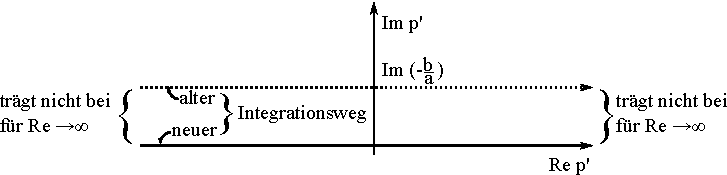
\includegraphics{191Integration}
\end{center}
Integrand analytisch ohne Singularit"aten im Gebiet zwischen altem und neuem Integrationsweg. Residuensatz $\Longrightarrow$
\begin{align}
\phi(x,t) & \stackrel{(190)}= \left( \frac{ d^2}{2 \pi^3} \right)^{\nicefrac 14} \frac 1 \hbar \underbrace{ \int_{-\infty}^\infty \dd p' \, \exp \left[ - ap'^2 + \frac {b^2}a - c \right]}_{ \sqrt {\frac \pi a} \exp \left[ \frac{b^2} a - c \right]} \\
\vert \phi(x,t) \vert^2 & = \frac d{\sqrt{ 2 \pi} \hbar^2} \frac 1 {\vert a \vert} \exp \left[ 2 \Re {\left( \frac{b^2}a - c \right)} \right] = \frac{d}{\sqrt{2 \pi} \hbar^2} \frac 1 {\vert a \vert} \exp \left[ 2 \Re  \frac{b^2a^*}{\vert a \vert^2} - c \right]
\end{align}
Mit 
\begin{align}
v & = \frac{p_0}m \quad \mathrm{und} \quad \Delta(t) = \frac{t \hbar}{2 m d^2}
\end{align}
ist
\begin{align}
\vert a \vert^2 & = \frac{d^4}{\hbar^4} + \frac{t^2}{4 m^2 \hbar^2} = - \frac{d^4}{\hbar^4} \left[ 1 + \Delta(t)^2 \right]
\end{align}
und
\begin{align}
2 \left( \Re \frac{b^2a^*}{\vert a \vert^2} - c \right) & = - \frac{ (x - vt)^2}{ 2 d (1 + \Delta(t^2))}
\end{align}
Einsetzen von (195) und (196) in (193):
\begin{align}
\vert \phi(x,t) \vert^2 = \frac 1{d \sqrt{2\pi}} \frac 1 {\sqrt{1+ \Delta(t)}^2} \exp \left[ - \frac{ ( x - v t)^2}{2 d^2 (1 + \Delta(t)^2) } \right]
\end{align}
Das Wellenpaket bewegt sich nach rechts mit Geschwindigkeit $v$ und "`zerflie"st, d.h. die Breite $\propto d(1 + \Delta t)$ w"achst linear mit $t$.

\psset{xunit=10pt}
\psset{yunit=100pt}
\begin{center}
\begin{pspicture}(20,0)(2,1.2)

\psplot[plotpoints=100]{0}{10}{2.65 x 5 sub 5 x sub mul exp}
\psplot[plotpoints=200]{0}{20}{1.2 x 15 sub 15 x sub mul exp 0.5 mul}
\psline{->}(0,0)(25,0)
\psline{->}(0,0)(0,1.2)
\uput[u](5,1){$t_1$}
\uput[u](15,0.5){$t_2 > t_1$}
\uput[l](0,1.1){$\vert \phi(x) \vert^2 $}
\uput[d](25,0){$x$}
\end{pspicture}
\end{center}
Zerflie"sen ist Folge der Impulsunsch"arfe in (189) analog zu einer Ladung Schrotkugeln.

Aus (197) finden wir
\begin{align}
\Braket{ X} = \Braket{ \phi, t | X | \phi, t} & = \int_{-\infty}^\infty \dd x \, x \vert \phi(x,t) \vert^2 = vt \\
(\Delta X)^2 = \sqrt{ \Braket{ \phi, t | X^2 - \Braket{X}^2 | \phi, t}} & = d \sqrt{1 + \Delta(t)^2}
\end{align}
mit Aufgabe 8, wobei $b = \sqrt 2 d (1 + \Delta(t))$.

$\Braket P$ und $(\Delta P)^2$ findet man am einfachsten aus (189):
\begin{align}
\begin{split}
\Braket P & = \int_{-\infty}^\infty \dd p \, p \vert \widetilde \phi(p,t) \vert^2 \\
& \stackrel{(189)}=  \left( \frac{ 2d^2}{\pi \hbar^2} \right) ^{\nicefrac 1 2} \int_{-\infty}^\infty \dd p \, p \exp \left[ - \frac{ - 2(p - p_0)^2 d^2}{\hbar^2} \right] \\
& = \left( \frac{ 2d^2}{\pi \hbar^2} \right) ^{\nicefrac 1 2} \int_{-\infty}^\infty \dd p' \, ( p' + p_0 ) \exp \left[ - \frac{ 2 p'^2 d^2}{\hbar^2} \right] \\
& = p_0 \\
& = \mathrm{unabh"angig \ von \ } t
\end{split} \\
(\Delta P)^2 & = \Braket{ P^2} - p_0^2 = \frac \hbar {2d} \quad \mathrm{mit \ Aufgabe \ 8}
\end{align}
(199), (201) $\Longrightarrow$
\begin{align}
\Delta X \Delta P & = \frac \hbar 2 \sqrt{ 1 + \Delta(t)^2}
\end{align}
$\Longrightarrow$ minimale Unsch"arfe f"ur $t=0$.

\subsection{Kastenpotential}
Betrachte
\begin{align}
V(x) & = - V_0 \theta(a - \vert x \vert), \quad V_0 > 0
\end{align}
\begin{center}
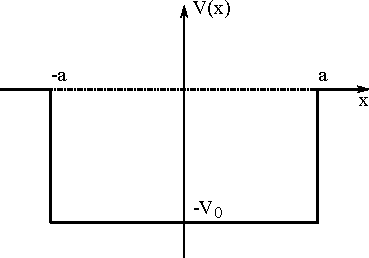
\includegraphics{203Katenpot}
\end{center}
Anwendung:
\begin{itemize}
\item abgeschirmte St"orstellen in Halbleitern
\item Kernphysik
\end{itemize}
Dimensionsloser Parameter:
\begin{align}
\xi & = \frac{\sqrt{2 m V_0} a}{\hbar}
\end{align}
Bindungszust"ande $\psi_n(x)$: $H \psi_n(x) = E_n \psi_n(x)$, also 
\begin{align}
- \frac{ \hbar^2}{2m} \frac{d^2}{dx^2} \psi_n(x) & = \left\{ \begin{aligned} & E_n \psi_n(x), && \vert x \vert > a \\ & (E_n + V_0) \psi_n(x), && \vert x \vert < a \end{aligned} \right\}
\end{align}
$\Longrightarrow \begin{cases} \psi_n''(x) \mathrm{ \ ist \ unstetig \ bei \ } \vert x \vert = a \mathrm{ \ mit \ Sprung \ } \pm V_0 \\
\psi_n'(x) \mathrm{ \ ist \ stetig \ mit \ Knick \ bei \ } \vert x \vert = a \\ \psi_n(x) \mathrm{ \ ist \ stetig} \end{cases}$
L"osung von (205) f"ur $\vert x \vert > a$:

\begin{tabular}{l l}
$E_n > 0$: & $\psi_n(x) \sim \sin (qx), \cos(qx)$ $\leadsto$ nicht normierbar $\leadsto$ Streuzust"ande. \\
$E_n < 0$: & $\psi_n(x) = \left\{ \begin{aligned} & N_n e^{\kappa_n x}, & & x < -a \\ &N'_n e^{- \kappa_n x}, && x > a \end{aligned} \right\}$ \hfill{} (206)\\
& mit $\kappa_n = \frac{ \sqrt{2m (-E_n)}}{\hbar}$ und Normierungskonstante $N_n, N_n'$ 
\end{tabular}
\setcounter{equation}{206}
Parit"atsoperator = Raumspiegelungsoperator:
\begin{align}
\mathcal P \psi(x) &= \psi(-x)
\end{align}
In unserem Fall:
\begin{align}
\begin{split}
H \mathcal P \psi(x) & = H \psi(-x) \\
& = \left[ - \frac{\hbar^2}{2m} \frac{d^2}{dx^2} + V(x) \right] \psi(-x)
\end{split} \notag\\
\begin{split}
\mathcal P H \psi(x) & = \left[ - \frac{\hbar ^2}{2m} \frac{d^2}{d(-x)^2} + V(-x) \right] \psi(-x) \\
& = H \psi(-x) \quad \mathrm{ wegen \ } V(-x) = V(x)
\end{split} \notag \\
\Longrightarrow [H, \mathcal P] &= 0
\end{align}
$\Longrightarrow$ Es gibt eine Basis aus gemeinsamen Eigenfunktionen von $H$ und $\mathcal P$.
\begin{align}
\mathcal P^2 = \dOne \ \Longrightarrow \ \mathrm{Eigenwerte \ } \pm 1
\end{align}
gerade Funktionen (EW 1): $\mathcal P \psi(x) = \psi(-x) = \psi(x)$:
\begin{center}
\psset{xunit=75pt}
\psset{yunit=75pt}
\begin{pspicture}(-1,0)(2,1.2)
\psplot[plotpoints=100]{-1}{1}{1 x x mul sub 0.5 exp}
\psline{->}(-1.5,0)(1.5,0)
\psline{->}(0,-0.2)(0,1.2)
\uput[l](0,1.1){$ \psi(x)$}
\uput[d](1.5,0){$x$}
\end{pspicture}
\end{center}
ungerade Funktionen (EW -1): $\mathcal P \psi(x) = \psi(-x) = - \psi (x)$
\begin{center}
\psset{xunit=75pt}
\psset{yunit=75pt}
\begin{pspicture}(-1,-1)(2,1.2)
\psplot[plotpoints=100]{-1}{1}{x 3 exp}
\psline{->}(-1.5,0)(1.5,0)
\psline{->}(0,-1.2)(0,1.2)
\uput[l](0,1.1){$ \psi(x)$}
\uput[d](1.5,0){$x$}
\end{pspicture}
\end{center}
gerade L"osungen: $N_n = N_n'$ in (206).

oszillierend $\psi_n(x) = C_n \cos(q_n x)$ f"ur $\vert x \vert \leq a$ mit
\begin{align}
q_n = \frac{ \sqrt{ 2m (E_n + V_0)}} \hbar
\end{align}
(206) und (210) $\Longrightarrow$ $-V_0 < E < 0$

Exponentielle L"osung ($E < - V_0$) in $\vert x \vert \leq a$ erf"ullen nicht die Stetigkeit von $\psi_n(x)$ und $\psi_n'(x)$ bei $x = \pm a$.

Stetigkeit: (206), (210) $\Longrightarrow$
\begin{align}
\psi_n(a) & = N_n e^{- \kappa_n a} \stackrel{!}= C_n \cos (q_n a) \\
\psi_n'(a) & = - N_n\kappa_n e^{- \kappa_n a}  \stackrel{!}= - C_n q_n \sin(q_n a)
\end{align}
$\frac{ - \mathrm{ (212)}}{\mathrm{(211)}} = \kappa_n = q_n \tan(q_n a)$
\begin{align}
\Longrightarrow \frac{\kappa_n }{q_n} & = \tan(q_n a)
\end{align}
Wegen 
\begin{align*}
\xi^2 & \stackrel{(204)}= \frac{a^2}{\hbar^2} 2 m V_0 \\
& = \frac{a^2}{\hbar^2} 2m (V_0 + E - E) \\
& \stackrel{(206)}= a^2 \left[ q_n^2 + \kappa_n^2 \right]
\end{align*}
bedeutet (213)
\begin{align}
\tan(q_n a) & = \frac{ \sqrt{\xi^2  - (q_n a)^2}}{q_n a}.
\end{align}
(214) bestimmt $q_n a$ und damit $E$. 

\begin{center}
\psset{xunit=0.5pt}
\psset{yunit=10pt}
\begin{pspicture}*(-100,-2)(520,10)
\psplot[plotpoints=100, linecolor=red]{0}{89}{x sin x cos div 0 max}
\psplot[plotpoints=100, linecolor=red]{180}{269}{x sin x cos div 0 max}
\psplot[plotpoints=100, linecolor=red]{360}{449}{x sin x cos div 0 max}
\psplot[plotpoints=100, linecolor=blue]{1}{419}{420 2 exp x 2 exp sub 0.5 exp x div}

\psline{->}(-20,0)(520,0)
\psline{->}(0,-1)(0,10)
\psline{-}(90,-0.25)(90,0.25)
\uput[d](90,0){$\frac \pi 2$}
\uput[l](80,5){$q_0$}
\psline[linestyle=dotted](90,-0.5)(90,10)
\psline{-}(180,-0.25)(180,0.25)
\uput[d](180,0){$\pi$}
\psline{-}(270,-0.25)(270,0.25)
\uput[d](270,0){$\frac 3 2 \pi$}
\uput[u](230,1.7){$q_2$}
\psline[linestyle=dotted](270,-0.5)(270,10)
\uput[d](360,-0.25){$2 \pi$}
\psline{-}(360,-0.25)(360,0.25)
\uput[d](450,0){$\frac 5 2 \pi$}
\uput[u](390,0.5){$q_4$}
\psline{-}(420,-0.25)(420,0.25)
\uput[d](420,0){$\xi$}
\psline{-}(420,-0.25)(420,0.25)
\psline[linestyle=dotted](450,-0.5)(450,10)
{ \red \uput[d](340,10){$\tan(q a)$} }
{ \blue \uput[d](160,7){$\frac{ \sqrt{\xi^2 - (q a)^2}}{a q}$} }
\uput[d](500,0){$qa$}
\end{pspicture}
\end{center}
Zahl der geraden L"osungen:
\begin{align}
n_g = \left[ \frac \xi \pi + 1 \right]
\end{align}
Energie-EW
\begin{align}
E_n \stackrel{(210)}= \frac{\hbar^2 q_n^2}{2m} - V_0
\end{align}
Insbesondere $E_0$ existiert immer und
\begin{align*}
-V_0 < E_n < \frac{\hbar^2 \pi^2}{8 m a^2}
\end{align*}
ungerade L"osungen: $N_n = - N_n'$ in (206) und
\begin{align}
\psi_n(x) & = S_n \sin(q_n x)
\end{align}
Stetigkeitsbedingungen liefern analog zu (211) bis (213):
\begin{align}
-\cot( q_n a) = \frac{\kappa_n}{q_n} = \frac{ \sqrt{ \xi^2 - (q_na)^2}}{q_n a}
\end{align}
\begin{center}
\psset{xunit=0.5pt}
\psset{yunit=10pt}
\begin{pspicture}*(-100,-2)(520,10)
\psplot[plotpoints=100, linecolor=red]{90}{179}{x cos x sin div -1 mul 0 max}
\psplot[plotpoints=100, linecolor=red]{270}{359}{x cos x sin div -1 mul 0 max}
\psplot[plotpoints=100, linecolor=blue]{1}{419}{420 2 exp x 2 exp sub 0.5 exp x div}
\psline{->}(-20,0)(520,0)
\psline{->}(0,-1)(0,10)
\psline{-}(90,-0.25)(90,0.25)
\uput[d](90,0){$\frac \pi 2$}
\uput[l](150,2.3){$q_1$}
\psline[linestyle=dotted](180,-0.5)(180,10)
\psline{-}(180,-0.25)(180,0.25)
\uput[d](180,0){$\pi$}
\psline{-}(270,-0.25)(270,0.25)
\uput[d](270,0){$\frac 3 2 \pi$}
\uput[u](310,1.3){$q_3$}
\psline[linestyle=dotted](360,-0.5)(360,10)
\uput[d](360,-0.25){$2 \pi$}
\psline{-}(360,-0.25)(360,0.25)
\uput[d](450,0){$\frac 5 2 \pi$}
\psline{-}(420,-0.25)(420,0.25)
\uput[d](420,0){$\xi$}
\psline{-}(420,-0.25)(420,0.25)
{ \red \uput[d](270,10){$\cot(q a)$} }
{ \blue \uput[d](90,10){$\frac{ \sqrt{\xi^2 - (q a)^2}}{a q}$} }
\uput[d](500,0){$qa$}
\end{pspicture}
\end{center}
Ungerade L"osungen gibt es also nur f"ur $\xi \geq \frac \pi 2$, also
$$\frac{2m V_0 a^2}{\hbar^2} > \frac{\pi^2}4$$

Lsg:

\psset{xunit=40pt}
\psset{yunit=100pt}
\begin{center}
\begin{pspicture}(-5,-1)(5,1)
\psgrid(0,0)(-4,-1)(4,1)
\psplot[plotpoints=100, linecolor=red]{-4}{4}{3.14 0.5 exp 1 mul 2 0 exp mul -0.5 exp 2.6 x x mul -0.5 mul exp mul }
\psplot[plotpoints=100, linecolor=blue]{-4}{4}{3.14 0.5 exp 1 mul 2 1 exp mul -0.5 exp 2.6 x x mul -0.5 mul exp mul 2 x mul mul}
\psplot[plotpoints=100, linecolor=green]{-4}{4}{3.14 0.5 exp 2 mul 2 2 exp mul -0.5 exp 2.6 x x mul -0.5 mul exp mul 4 x 2 exp mul 2 sub mul}
\psplot[plotpoints=100, linecolor=yellow]{-4}{4}{3.14 0.5 exp 6 mul 2 3 exp mul -0.5 exp 2.6 x x mul -0.5 mul exp mul 8 x 3 exp mul 12 x mul sub mul}
\uput[dr](0,1){$\psi_n(x)$}
\uput[dl](4,0){$\frac x {x_0}$}
\red \uput[r](3,-0.3){$n=0$}
\blue \uput[r](3,-0.4){$n=1$}
\green \uput[r] (3,-0.5){$n=2$}
\yellow \uput[r](3,-0.6){$n=3$}

\end{pspicture}
\end{center}

\begin{tabular}{c | c | c | c }
Zustand & $q_n a \in$ & Symmetrie & Knotenzahl \\
\hline
$n=0$ & $[0, \frac \pi 2]$ & gerade & $0$ \\
$n=1$ & $[\frac \pi 2, \pi]$ & ungerade & $1$ \\
$n=2$ & $[\pi, \frac 3 2 \pi]$ & gerade & $2$
\end{tabular}

\setcounter{section}{2}
\setcounter{subsection}{2}
\subsection{Harmonischer Oszillator}
Betrachte
\setcounter{equation}{218}
\begin{align}
H & = \frac{P^2}{2m} + \frac{m \omega^2 X^2}{2},
\end{align}
d.h. Federkonstante $\kappa = m \omega^2$.

Algebraische L"osung (H. Born, N. Wiener):
\begin{align}
x_0 & = \sqrt {\frac{\hbar}{m \omega}} \\
\Longrightarrow H & = \underbrace{\hbar \omega}_{\mathrm{char. \  Energie}} \left[ \frac 12 \frac{P^2 x_0^2}{\hbar^2} + \frac 12 \left( \frac X {x_0} \right)^2 \right]
\end{align}
Vernichtungsoperator (= Absteigeoperator), annihilation op:
\begin{align}
a & = \frac1 {\sqrt 2} \left( \frac X {x_0} + i \frac {P x_0}{\hbar} \right)
\end{align}
Erzeugungsoperator (= Aufsteigeoperator), creation op
\begin{align}
a^\dagger & = \frac1 {\sqrt 2} \left( \frac X {x_0} - i \frac {P x_0}{\hbar} \right)
\end{align}
Es gilt f"ur den Kommuator:
\begin{align}
\begin{split}
[a, a^\dagger] & = \frac 12 \frac i \hbar \left( \left[ P x_0, \frac X {x_0} \right] - \left[ \frac X {x_0}, P x_0 \right] \right) \\
& \stackrel{(110)}= \frac 12 \frac i \hbar ( - i \hbar - i \hbar) = \dOne
\end{split}
\end{align}
Besetzungszahl-Operator: 
\begin{align}
N &  a^\dagger a
\end{align}
(222) und (223) liefern:
\begin{align}
N & = \frac 12 \left( \frac X {x_0} - i \frac {P x_0} \hbar \right) \left( \frac X {x_0} + i \frac{P x_0} \hbar \right) \notag \\
& = \frac 12 \left( X^2 {x_0^2} + \frac{P^2 x_0^2}{\hbar^2} + \frac i \hbar \left[ x, P \right] \right)  \notag \\
& = \frac H {\hbar \omega} - \frac12 \notag \\
\Longrightarrow H & = \hbar \omega ( N + \frac 12)
\end{align}
Also: Eigenzust"ande von $H$ sind Eigenzust"ande von $N$ und umgekehrt.
\begin{align}
N \ket n & = n \ket n \quad \mathrm{mit \ } n \in \RR \mathrm{ \ wegen \ } N = N^\dagger
\end{align}
$\ket n $ ist ein Eigenket zum Eigenwert $n$.
\begin{align}
\begin{split}
n & = n \braket {n | n } \\
& = \Braket { n | N | n } \\
& = \Braket{ n | a^\dagger a | n } \\
& = \Braket {an | an} \\
& = \left\Vert \ket{an} \right\Vert^2 \\
& \geq 0 
\end{split} \\
\begin{split}
[N, a^\dagger] & = [a^\dagger a, a^\dagger] \\
& = a^\dagger \underbrace{ [a, a^\dagger] }_{=1} + \underbrace{ [a^\dagger, a^\dagger]}_{=0} a \\
& = a^\dagger
\end{split} \\
\begin{split}
[N, a] & = [a^\dagger, N]^\dagger \\
& = \left( -a^\dagger \right)^\dagger \\
& = -a
\end{split}
\end{align}
Betrachte $a \ket n$:
\begin{align}
\begin{split}
N a \ket n & = \left( [N, a] + aN \right) \ket n \\
& = - a \ket n + an \ket n \\
& = (n-1) a \ket n 
\end{split}
\end{align}
$\Longrightarrow$ $a \ket n $ ist Eigenket zu $N$ mit Eigenwert $n-1$ oder $a \ket n = 0$.

Ist $a \ket n = 0$, so ist $N \ket n = a^\dagger a \ket n =  0 \ \Longrightarrow n = 0$,
\begin{align}
N \ket 0 = 0
\end{align}
Achtung: $\ket 0 \neq \underbrace{0}_{\mathrm{Nullvektor}}$.

Aus (231) folgt durch volls"andige Induktion, dass $a^k \ket n$ Eigenvektor zu $N$ mit Eigenwert $n-k$ ist, au"ser wenn $k-n \in \NN$. Wegen (228) muss f"ur Eigenwerte $n-k \geq 0$ sein. W"are $n \notin \NN_0$, so k"onnten wir mit hinreichend gro"sem $k$ Gleichung (228) verletzen 
\begin{align}
\Longrightarrow n \in \NN_0
\end{align}
\emph{Konstruktion der Eigenkets}: 

Zwei M"oglichkeiten:
\begin{1aufz}
\item Der Grundzustand $\ket 0$ ist nicht entartet
\item Der Grundzustand ist entartet
\end{1aufz}
Welche M"oglichkeit realisiert ist, h"angt vom Hilbertraum $\mathcal H$ ab.
\begin{align*}
(229) \Longrightarrow N a^\dagger \ket n & = a^\dagger \underbrace{ N \ket n }_{n \ket n} + \underbrace{ [N, a^\dagger]}_{a^\dagger} \ket n \\
& = (n+1))\underbrace{ a^\dagger \ket n}_{\mathrm{EZ \ zu \ } N \mathrm{ \ mit \ EW \ } n+1}
\end{align*}
Normierung:
\begin{align*}
\Vert a^\dagger \ket n \Vert^2 & = \braket { a^\dagger n | a^\dagger n} \\
&  = \braket { n | a a^\dagger | n } \\
& = \braket{ n | \underbrace{ [ a, a^\dagger]}_{=1} | n } + \braket{ n | \underbrace{ a^\dagger a }_{=N} | n } \\
& = 1+n
\end{align*}
$\Longrightarrow$ $\ket {n+1} = \frac1{\sqrt{n+1}} a^\dagger \ket n $ ist normiert \hfill (234)
\setcounter{equation}{234}

Im Fall 1 (nichtentarteter Grundzustand $\ket 0$) definierten wir rekursiv:
\begin{align}
\begin{split}
\ket n & \stackrel{(234)}= \frac 1 {\sqrt{n}} a^\dagger \ket {n-1} \\
& = \frac 1 {\sqrt{n (n-1)}} a^{\dagger 2} \ket {n-2} \\
& = \frac1 {\sqrt{n!}} a^{\dagger n } \ket 0
\end{split}
\end{align}
Weiter
\begin{align}
\begin{split}
a \ket n & \stackrel{(234)}= \frac 1 {\sqrt n} a a^\dagger \ket{n-1} \\
& = \frac 1{\sqrt n } \underbrace{ [a, a^\dagger]}_{=1} \ket{n-1} + \frac 1 {\sqrt{n}} \underbrace{ a^\dagger a}_{=N} \ket{n-1} \\
& = \frac 1{\sqrt{n}} n \ket{n-1} \\
& = \sqrt n \ket{n-1}
\end{split}
\end{align}
Zuammenfassung von (234) und (236):
\begin{align}
\begin{split}
a^\dagger \ket n & = \sqrt{ n+1} \ket{n+1} \\
a \ket n & = \sqrt n \ket {n-1}
\end{split}
\end{align}
und
\begin{align}
a^n \ket n = \sqrt{n!} \ket 0
\end{align}
Haben wir im Fall 1 mit (235) alle EZ gefunden? Ja!

\emph{Beweis:} Angenommen, es gibt au"ser $\ket n$ in (235) einen weiteren Ket $\ket {n'}$ mit $N \ket {n'} = n \ket {n'}$ und $\braket{ n | n'} = 0$, so ist $n$ entartet. Wegen (231) ist $a^n \ket {n'}$ EZ von $N$ zu $n=0$. Da $n=0$ nicht entartet ist, folgt:
\begin{align}
&& a^n \ket {n'} &= e^{i \phi} \sqrt{n!} \ket 0 \\
\Longrightarrow && \frac1{n!} a^{\dagger n} a^n \ket{n'} & = e^{i \phi} \frac1{\sqrt{n!}} a^{\dagger n} \ket 0 \notag \\
&& & \stackrel{(235)}= e^{i \phi} \ket n \notag \\
\Longrightarrow && \frac1{n!} \underbrace{ \Braket{ n' | a^{\dagger n } a^n | n'} }_{\Vert \ket{a^n n'} \Vert^2} & = e^{i \phi} \braket{n' | n} \notag\\
&& & \stackrel{\mathrm{Ann.}}= 0\notag
\end{align}
$\Longrightarrow a^n \ket{n'} = 0$. Wid. zu (239) \hfill $\square$

Im Fall 2 haben wir Grundzust"ande 
$$\ket{ 0, \lambda},  \ \lambda = \mathrm{Entartungsindex}$$
Analog findet man:
$$ \ket{n , \lambda} = \frac1{\sqrt {n!}} a^{\dagger n } \ket{ 0, \lambda}$$
sind alle EZ zum Eigenwert $n$ von $N$. 

Wegen (226) sind die Energieeigenwerte 
\begin{align}
E_n = \hbar \omega( n + \frac 12 ), \quad n \in \NN_0
\end{align}


\psset{xunit=20pt}
\psset{yunit=20pt}
\begin{center}
\begin{pspicture}(0,0)(5,5)
\psplot[plotpoints=100]{-3}{3}{x x mul 2 div}
\psplot[plotpoints=100]{-2.5}{2.5}{x x mul 2 div 0.5 max}
\psplot[plotpoints=100]{-2.5}{2.5}{x x mul 2 div 1.5 max}
\psplot[plotpoints=100]{-2.5}{2.5}{x x mul 2 div 2.5 max}
\psline{->}(-4,0)(4,0)
\psline{->}(0,0)(0,5)

\psline{-}(-0.25,1)(0.25,1)
\uput[r](0.25, 1){$1$}
\psline{-}(-0.25,2)(0.25,2)
\uput[r](0.25, 2){$2$}
\psline{-}(-0.25,3)(0.25,3)
\uput[r](0.25, 3){$3$}
\uput[r](1,0.5){$E_0$}
\uput[r](1.6,1.5){$E_1$}
\uput[r](2.1,2.5){$E_2$}
\psline{-}(-2,-0.25)(-2,0.25)
\uput[d](-2,-0.25){$-2$}
\psline{-}(-1,-0.25)(-1,0.25)
\uput[d](-1,-0.25){$-1$}
\psline{-}(1,-0.25)(1,0.25)
\uput[d](1,-0.25){$1$}
\psline{-}(2,-0.25)(2,0.25)
\uput[d](2,-0.25){$2$}
\uput[d](4,0){$x$}
\uput[r](0,5){$\frac{V(x)}{\hbar \omega}$}
\end{pspicture}
\end{center}
Streuzust"ande gibt es nicht!

$\mathcal H = L^2[\RR]$, Ortsdarstellung.
$$a \ket 0 \stackrel{(237)}= 0 $$
Also
$$0 = \Braket{ x | a | 0 } \stackrel{(222)}= \frac1{\sqrt 2} \Braket{ x | \frac X {x_0} + i \frac{P x_0 }\hbar | 0 } = \frac 1{\sqrt 2} \left[ \frac x {x_0} + i \frac{ x_0}\hbar \frac \hbar i \frac d {dx} \right] \underbrace{ \Braket{ x| 0}}_{\psi_0(x)}$$
$\Longrightarrow$
\begin{align}
\left[ \frac d{dx} + \frac x{x_0^2} \right] \psi_0(x) & 0 
\end{align}
(241) ist eine DGL 1. Ordnung. Standard-L"osungsweg:

Ansatz: 
$$e^{f(x)} \left[ \frac d{dx} + \frac x{x_0^2} \right] \psi_0(x) = 0$$
$\Longrightarrow$
$$\Big[ \frac d {dx} - \underbrace{f'(x) + \frac x {x_0^2} }_{=0} \Big] e^{f(x)} \psi_0(x) = 0$$
W"ahle $f'(x) = \frac x {x_0^2}$, also $f(x) = \frac12 \left( \frac x{x_0} \right)^2$
$$\Longrightarrow \frac d{dx} \left[ e^{\frac 12 \left( \frac x{x_0} \right)^2} \psi_0(x) \right] =0, \ \mathrm{ also \ } \psi_0(x) = C e^{-\frac12 \left( \frac x{x_0} \right)^2}$$
Normierung:
$$1 = \Braket {0 | 0 } = \vert C \vert^2 \int_{-\infty}^\infty \dd x \, e^{- \left( \frac x{x_0} \right)^2} = \vert C \vert^2 x_0 \sqrt \pi$$
W"ahle $C = (x_0 \sqrt \pi)^{-\frac 12}$

$\Longrightarrow$ Grundzustand-Wellenfunktionen:
\begin{align}
\psi_0(x) = (x_0 \sqrt \pi)^{-\frac 12 } e^{-\frac 12 \left( \frac x {x_0} \right)^2}
\end{align}
"Ubrigen: $n > 0$
$$\psi_n(x) = \Braket{ x | n } \stackrel{(235)}= \frac 1{\sqrt{n!}} \Braket{ x | a^{\dagger n} | 0} = \frac1{\sqrt{n!}} \frac1{\sqrt{2^n}} \left[ \frac x{x_0} - x_0 \frac d {dx} \right]^n \psi_0(x)$$
Dimensionslose Variable
$$\xi := \frac x{x_0}$$
Damit gilt:
\begin{align}
\begin{split}
\psi_n(x_0 \xi) & = \frac1{\sqrt{n!}} \frac1{\sqrt{2^n}} \left[ \xi - \frac d{d \xi} \right]^n \psi_0(x_0 \xi) \\
& \stackrel{(242)}= (x_0 \sqrt \pi)^{-\frac12} \frac1{\sqrt n!} \frac1{\sqrt2^n} \left[ \xi -  \frac d {d\xi} \right]^n e^{-\frac {\xi^2} 2} \\
& = (x_0 \sqrt \pi n! 2^n)^{-\frac 12} H_n(\xi) e^{-\frac {\xi^2}2}
\end{split}
\end{align}
mit
\begin{align}
H_n(\xi) & := e^{\frac \xi 2} \left[ \xi - \frac d {d\xi} \right]^n e^{-\frac {\xi^2}2}
\end{align}
Operator-Identit"at:
\begin{align}
A_\xi &:= e^{-\frac {\xi^2}2} \left( \xi - \frac d{d\xi} \right) e^{\frac {\xi^2}2} = - \frac d{d\xi},
\end{align}
denn:
\begin{align*}
A_\xi \psi(\xi) & = e^{- \frac{\xi^2}2} \left( \xi - \frac d {d\xi} \right) e^{\frac{\xi^2}2} \psi(\xi) \\
& = e^{-\frac{\xi^2}2} \left[ \xi e^{\frac{\xi^2}2} \psi(\xi) - \xi e^{\frac{\xi^2}2}\psi{\xi} - e^{\frac{\xi^2}2 } \frac d{d\xi} \psi(\xi) \right] \\
& = - \frac d{d\xi} \psi(\xi)
\end{align*}
(245) $\Longrightarrow$
$$ (-1)^n \frac{d^n}{d\xi^n} = A_\xi^n
 = e^{-\frac{\xi^2}2} \left[ \xi - \frac d{d\xi} \right]^n e^{\frac {\xi^2}2}$$
Einsetzen von (245) in (244):
\begin{align}
H_n(\xi) & = (-1)^n e^{\xi^2} \frac{d^n}{d \xi^n} e^{- \xi^2}
\end{align}
ist die Definitions-Gleichung der \emph{Hermite-Polynome:}
\begin{align}
\begin{split}
H_0(\xi) & = 1 \\
H_1(\xi) & = 2 \xi \\
H_2(\xi) & = 4 \xi^2 - 2 \\
H_3(\xi) & = 8 \xi^3 - 12 \xi \\
H_4(\xi) & = 16 \xi^4 - 48 \xi^2 + 12 \\
H_5(\xi) & = 32 \xi^5 - 160 \xi^3 + 120 \xi
\end{split}
\end{align}
Aus $\delta_{nm} = \braket{n | m} = \int_{-\infty}^\infty \dd x ß,k \psi_n(x)^* \psi_m(x)$ folgen mit (243) die \emph{Orthogonalit"atsrelationen}
\begin{align}
\int_{-\infty}^\infty \dd \xi \, e^{-\xi^2} H_n(\xi) H_m(\xi) & =  \sqrt \pi 2^n n! \delta_{nm}
\end{align}
Aus $\sum_{n=0}^\infty \ket n \bra n = \dOne$ folgt die \emph{Vollst"andigkeitsrelation}
\begin{align}
\begin{split}
\sum_{n=0}^\infty \psi_n(x) \psi_n^*(x') & = \sum_{n=0}^\infty \braket{ x | n } \braket{ n | x} \\
& = \braket{ x | x'} \\
& = \delta(x - x')
\end{split}
\end{align}
Mit (243)
\begin{align}
\sum_{n=0}^\infty H_n(\xi) H_n(\xi') & = \sqrt \pi n! 2^n e^{\xi^2} \delta( \xi - \xi')
\end{align}
Weitere Eigenschaftende:

Erzeugende Funktionen:
\begin{align}
e^{-t^2 - it \xi} & = \sum_{n=0}^\infty \frac 1{n!} t^n H_n(\xi)
\end{align}
Hermitescher DGL:
\begin{align}
\left[ \frac{d^2}{d\xi^2} - 2\xi \frac{d}{d\xi} + 2n \right] H_n(\xi) = 0
\end{align}

\begin{center}
\begin{tabular}{ l l l}
klassische Physik: & niedrigste Energie & $E = 0$ \\
QM: & \ldots & $E_0 = \frac{\hbar \omega}2$ "`Nullpunktsenergie
\end{tabular}
\end{center}
Ein Zustand mit $E=0$ w"urde $\Delta X \Delta P \geq \frac \hbar 2$ verletzen.

Inverse von (222)/(223):
\begin{align}
X & = \frac{x_0}{\sqrt 2} (a + a^\dagger) \\
P & = \frac i {\sqrt 2} ( a^\dagger - a)
\end{align}
Damit folgt:
\begin{align*}
\Braket{ n | X | n } & \stackrel{(253)}= \frac{x_0}{\sqrt 2} \Braket{n | a + a^\dagger | n} \\
& \stackrel{(237)}= \frac{x_0}{\sqrt 2} \Big[ \sqrt n \underbrace{\Braket{ n | n-1}}_{=0} + \sqrt{n+1} \underbrace{\Braket{ n | n+1}}_{=0}  \Big]\\
& = 0.
\end{align*}
Ebenso $\Braket{ n | P | n } \stackrel{(254)}= 0$
\begin{align}
\begin{split}
(\Delta X)^2 & = \Braket{ n | X^2 | n } \\
& \stackrel{(253)}= \frac{x_0^2}2 \Braket{ n | (a + a^\dagger)^2 | n } \\
& = \frac{x_0^2}2 \Big[ \underbrace{ \Braket{n | a^2 | n}}_{=0} +  \underbrace{ \Braket{ n | a a^\dagger + a^\dagger a | n }}_{= \Braket{ n | [a, a^\dagger] + 2 N | n }= 1} + \underbrace{ \Braket{ n | a^\dagger | n }}_{=0} \Big] \\
& = \frac{x_0^2}2 \left[ \Braket{n | n} + 2 \Braket{ n | N | n} \right] \\
& = \frac{x_0^2}2 (2n+1)
\end{split} \\
\begin{split}
(\Delta P)^2 & = \Braket{ n | P^2 | n } \\
& \stackrel{(254)}= - \frac{\hbar^2}{2 x_0^2} \braket{ n | ( a^\dagger - a)^2 | n } \\
& = - \frac{\hbar^2}{2 x_0^2} \Braket{ n | a^\dagger a + a a^\dagger | n } \\
& = \frac{hbar^2}{2 x_0^2} (2n + 1)
\end{split} \\
\Longrightarrow \Delta X \Delta P & = \frac \hbar 2 (2n+ 1)
\end{align}
$\Longrightarrow$ Grundzustand $\ket 0$ hat minimale Unsch"arfe

\psset{xunit=40pt}
\psset{yunit=100pt}
\begin{center}
\begin{pspicture}(-5,-1)(5,1)
\psgrid(0,0)(-4,-1)(4,1)
\psplot[plotpoints=100, linecolor=red]{-4}{4}{3.14 0.5 exp 1 mul 2 0 exp mul -0.5 exp 2.6 x x mul -0.5 mul exp mul }
\psplot[plotpoints=100, linecolor=blue]{-4}{4}{3.14 0.5 exp 1 mul 2 1 exp mul -0.5 exp 2.6 x x mul -0.5 mul exp mul 2 x mul mul}
\psplot[plotpoints=100, linecolor=green]{-4}{4}{3.14 0.5 exp 2 mul 2 2 exp mul -0.5 exp 2.6 x x mul -0.5 mul exp mul 4 x 2 exp mul 2 sub mul}
\psplot[plotpoints=100, linecolor=yellow]{-4}{4}{3.14 0.5 exp 6 mul 2 3 exp mul -0.5 exp 2.6 x x mul -0.5 mul exp mul 8 x 3 exp mul 12 x mul sub mul}
\uput[dr](0,1){$\psi_n(x)$}
\uput[dl](4,0){$\frac x {x_0}$}
\red \uput[r](3,-0.3){$n=0$}
\blue \uput[r](3,-0.4){$n=1$}
\green \uput[r] (3,-0.5){$n=2$}
\yellow \uput[r](3,-0.6){$n=3$}

\end{pspicture}
\end{center}

klassisch: Aufenthalt nur dort, wo $E \geq V$ ist, also $\left\vert \frac x {x_0} \right\vert \leq \sqrt{ 2n +2}$  f"ur den $n$-ten Energiezustand $E_n$.

QM: $\vert \psi_n(x) \vert^2 > 0$ auch f"ur $\vert x \vert > \sqrt {2n + 2}$

\subsubsection*{Zeitentwicklung}
\begin{align}
\begin{split}
\mathrm{Schr"odinger-Bild}: & \  \Ket{n, t} = e^{- \frac i n E_n t} \Ket n \\
\mathrm{Heisenberg-Bild}: & \  a(t=0)=a
\end{split} 
\end{align}
Aus (182) folgt
\begin{align}
\begin{split}
\frac d{dt} a & = \frac i \hbar [H, a] \\
& \stackrel{\mathrm{(226)}}= i \omega \left[ N + \frac 12, a\right] \\
& = i \omega [N, a] \\
& \stackrel{\mathrm{(239)}}=- i \omega a
\end{split}
\end{align}
Au"serdem
\begin{align}
\begin{split}
a(t) & = a(0) e^{ i \omega t} \\
a^\dagger(t) & = a^\dagger(0) e^{i \omega t}
\end{split}
\end{align}
Also
\begin{align}
\begin{split}
\Longrightarrow X(t) & \stackrel{(253)}= \frac {x_0} {\sqrt 2} (a e^{-i \omega t} + a^\dagger e^{i \omega t}) \\
& = \frac{x_0}{\sqrt 2} \left[ ( a + a^\dagger) \cos(\omega t) + (a^\dagger - a) i \sin(\omega t) \right] \\
& \stackrel{(253), (254)}= X \cos (\omega t) + \frac{x_0^2}{\hbar} P \sin(\omega t) \\
& \stackrel{(220)}= X \cos(\omega t) +  \frac{1}{m \omega} P \sin(\omega t)
\end{split}
\end{align}
wobei $X = X(0)$ und $P = P(0)$.

Analog:
\begin{align}
P(t) = P \cos(\omega t) - m \omega X \sin(\omega t)
\end{align}
$\Longrightarrow$ klassische Bewegungsgleichung des harmonischen Oszillators

Welche Zust"ande zeigen die Schwingungen des klassischen Oszillators?

Nicht die Energie-Eigenzust"ande:
\begin{align*}
\Braket{ n | X(t) | n} & \stackrel{(181),(165)}= \Braket{n | e^{\frac i \hbar H t} X e^{- \frac i \hbar H t} | n } \\
& = e^{\frac i \hbar E_n t} \Braket{n | X | n } e^{- \frac i \hbar E_n t} \\
& = \Braket{ n | X | n },
\end{align*}
jedoch 
$$ \Braket{ \lambda | X(t) | \lambda} = \sqrt 2 x_0 A \cos(\omega t - \lambda)$$
f"ur sogenannte \emph{koh"arente Zust"ande} $\ket \lambda$.

\subsubsection*{Nachtrag zum Thema Heisenberg-Bild:}

$$H = \frac{P^2}{2m} + V(X)$$
(183), (189) implizieren f"ur jeden Zustand $\psi$:
\begin{align}
\frac d {dt} \Braket{ \psi | X | \psi} & = \frac 1m \Braket{ \psi | P | \psi} \notag \\
\frac d {dt} \Braket{ \psi | P |  \psi}  &  =  - \Braket{ \psi | \frac {\partial V}{\partial x} | \psi } \notag \\
\Longrightarrow m \frac{d^2}{dt^2} \Braket{X} & =  \frac{d \Braket P }{ d t} = - \Braket{ \frac \partial {\partial x} V(X)}
\end{align}
(263) hei"st \emph{Ehrenfest'sches Theorem}.

Damit $\Braket {\psi | X | \psi}$ die klassischen Bewegungsgleichung erf"ullt, muss
\begin{align}
\Braket{\psi | \frac{\partial V}{\partial x} | \psi} & = \frac{\partial}{\partial x} V(\Braket{ \psi | X | \psi})
\end{align}
gelten. (264) gilt sogar f"ur alle $\ket \psi \in \mathcal H$, wenn $V$ h"ochstens quadratisch ist.

\section{Drehung, Drehimpuls, Spin}

\subsection{Drehungen und ihre Erzeuger}

passive Drehung in $\RR^3$ um Achse $\vv n$ (mit $\vv n^2 = 1$) mit Winkel $\phi$:

Aufgabe 6e): Vektor $\vv a \in \RR^3$ wird in $\vv {a_\phi}$ gedreht, wobei 
\begin{align}
\vv {a_\phi} & = \cos \phi \vv a + (1 - \cos \phi) ( \vv a \cdot \vv n ) \vv n -  \sin \phi( \vv n \times \vv a)
\end{align}
Kurznotation: $\vv \phi = \phi \vv n$ beschreibt die Drehung.

Suche Matrix $R(\vv \phi) \in\RR^{3 \times 3}$ mit 
\begin{align}
\vv{a_\phi} = R(\phi) \vv a \quad \mathrm{f"ur \ alle \ } \vv a \in \RR^3
\end{align}
(265) $\Longrightarrow$
\begin{align*}
a_{\phi k} & = \cos \phi a_k + (1 - \cos \phi) \left( \sum_{n=1}^3 a_m n_m \right) n_k - \sin \phi \left( \sum_{m,l =1}^3 \eps_{klm} n_l a_m \right) \\
& \stackrel{(266)}= \sum_{m=1}^3 \left[ R(\vv \phi) \right] _{km} a_m
\end{align*}
$\Longrightarrow$
\begin{align}
\left[ R( \vv \phi) \right]_{km} & =  \cos \phi \delta_{km} + (1- \cos \phi) n_k n_m - \sin \phi \sum_{l=1}^3 \eps_{klm} n_l, \mathrm{\ d.h.} \\
R(\vv \phi)  & = 
\matr{
\cos \phi + (1- \cos \phi) n_1^2 & (1- \cos \phi) n_1 n_2 + \sin n_3 & (1- \cos \phi) n_1 n_3 - \sin \phi n_2 \\
(1- \cos \phi) n_1 n_2 - \sin \phi n_3 & \cos \phi + (1- \cos \phi) n_2^2 &  (1- \cos \phi) n_2 n_3 + \sin \phi n_1 \\
(1-\cos \phi) n_1 n_3 + \sin \phi n_2 & (1- \cos \phi) n_2 n_3 - \sin n_1 & \cos \phi + (1- \cos \phi) n_3^2
}
\end{align}
Spezialfall: Drehung um $z$-Achse: $\vv n = (0, 0, 1)^\top$
\begin{align}
R\left( \matr{ 0 \\ 0 \\ \phi } \right) & = \matr{ \cos \phi & \sin \phi & 0 \\ - \sin \phi & \cos \phi & 0 \\ 0 & 0 & 1 }
\end{align}
Drehmatrizen sind orthogonal: $R(\vv \phi)^\top R(\vv \phi) = \dOne$ mit $\det R(\vv \phi) = 1$. Auch: Alle Matrizen $T$ mit $R^\top R = 1$ und $\det R = 1$ sind Drehmatrizen.

Bestimmung von $\phi$ und $\vv n$ aus $R(\phi)$:
\begin{itemize}
\item $\vv n$ ist Eigenvektor zum EW 1
\begin{align}
R(\vv \phi) \vv n = \vv n
\end{align}
\item $\phi$ kann "uber die Spur von $R(\vv \phi)$ berechnet werden:
\begin{align}
\tr R(\vv \phi) & \stackrel{(267)}= \cos \phi \underbrace{ \tr \dOne}_{=3} + (1 - \cos \phi) \underbrace{\sum_k n_k^2 }_{=1} = 1 + 2 \cos \phi
\end{align}
\end{itemize}
Die Menge aller Drehmatrizen bildet eine \emph{Lie-Gruppe}.

\subsubsection*{Definitionseigenschaften einer Lie-Gruppe}

\begin{1aufz}
\item Es gibt ein Einselement $\dOne$:
$$R(\vv \phi) \dOne = \dOne R(\vv \phi) = R( \vv \phi)$$
\item $R(\vv{\phi_1} ) \cdot R( \vv {\phi_2})$ ist Drehmatrix und in $R(\vv{\phi_3}) = R(\vv{\phi_1})R(\vv{\phi_2})$ ist $\vv{\phi_3}$ eine stetige Funktion von $\vv{\phi_1}$ und $\vv {\phi_2}$ (sogar analytisch)
\item $R^{-1}(\vv{\phi_1})$ ist Drehmatrix 
\item $\big( R(\vv{\phi_1}) R(\vv{\phi_2}) \big) R(\vv{\phi_3}) = R(\vv{\phi_1}) \big( R(\vv{\phi_2})R(\vv{\phi_3}) \big)$
\end{1aufz}
Die Lie-Gruppe der Drehung im $\RR^3$ hei"st $\mathrm{SO}(3)$. Dabei steht "`S"' f"ur "`speziell"', d.h. $\det R = 1$, "`O"' f"ur "`orthogonal"' und 3 f"ur den $\RR^3$.

Infinetissimale Drehung: $\delta \phi \ll 1$ in (267):
\begin{align}
R( \delta \phi \vv n) = \dOne + \delta \phi i \vv n \cdot  \omega = \dOne + i \delta \phi \sum_{l=1}^3 n_l \omega^{(l)}
\end{align}
wobei
\begin{align}
i \omega_{km}^{(l)}  = - \eps_{klm}
\end{align}
also
\begin{align}
i \omega^{(1)} = \matr{0 & 0 & 0 \\ 0 & 0 & 1 \\ 0 & -1 & 0}, \\
i \omega^{(2)} = \matr{ 0 & 0 & -1 \\ 0 & 0 & 0 \\ 1 & 0 & 0 } \\
i \omega^{(3)} = \matr{ 0 & 1 & 0 \\ -1 & 0 & 0 \\ 0 & 0 & 0 }
\end{align}
Die $\omega^{(l)}$ hei"sen \emph{Generatoren} der $\mathrm{SO}(3)$.

Aufbau einer endlichen Drehung aus infinitesimalen Drehungen: $\delta \phi = \frac \phi N$. Dann:
\begin{align}
[ R( \delta \phi \vv n) ]^N & = \left[ 1 + i \frac \phi N \vv n \vv \omega\right]^N \notag \\
\Longrightarrow R(\vv \phi)&  = \lim_{N \rightarrow \infty} \left[  R \left( \frac \phi N \vv n \right) \right]^N = e^{i \phi \vv n \vv \omega} = e^{i \vv \phi \vv \omega}
\end{align}
das ist eleganter als (267).

Alternativ: Euler-Winkel:
\eqn{
R(\alpha, \beta, \gamma) = R( \alpha \vv{e_z}) R( \beta \vv{e_y}) R( \gamma \vv{e_z})
}
Die Generatoren der $\mathrm{SO}(3)$ erf"ullen:
\eqn{ \left[ \omega^{(j)}, \omega^{(k)} \right] = i \sum_{l=1}^3 \eps_{jkl} \omega^{(l)}}
Beweis:
\eqnnon{
\left[ \omega^{(j)}, \omega^{(k)} \right]_{ln} & = \sum_{m=1}^3 \left[ \omega^{(j)}_{lm} \omega_{mn}^{(k)} - \omega_{lm}^{(k)} \omega_{mn}^{(j)} \right] \\
& \stackrel{(273)}= - \sum_{m=1}^3 ( \eps_{ljm} \eps_{mkn} - \eps_{lkm} \eps_{mjn} ) \\
& = - ( \delta_{lk} \delta_{jn} - \delta_{ln} \delta_{jk} - \delta_{lj} \delta_{kn} + \delta_{ln}\delta_{jk} ) \\
& = - \sum_{m=1}^3 \eps_{jkm} \eps_{lmn} \\
& = i \sum_{m=1}^3 \eps_{jkm} \omega_ln^{(m)}
}
Der von $\set{ \omega^{(1)}, \omega^{(2)}, \omega^{(3)} }$ aufgespannte Vektorraum hei"st Lie-Algebra $\mathrm{so}(3)$.

Also: $\vv q \omega \in \mathrm{so}(3) \Longrightarrow e^{i \vv q \vv \omega} \in \mathrm{SO}(3)$.

Allgemein: Ein Satz $\set{ \omega^{(1)}, \ldots, \omega^{(n)} }$ von Matrizen oder linearen Operatoren bildet eine Lie-Algebra, wenn
\eqn{
[\omega^{(j)}, \omega^{(k)} ] & = i \sum_l f_{jkl} \omega^{(l)}
}
mit $f_{jkl} \in \CC$.

Die Zahlen $f_{jkl}$ hei"sen \emph{Strukturkonstanten} der Lie-Algebra bzw. Lie-Gruppe

$\set{ e^{i \vv q \vv \omega} }$ ist dann Lie-Gruppe.

Betrachte: $\omega^{(j)} \longrightarrow \omega^{(j)'}$ mit
$$[\omega^{(j)'}, \omega^{(k)} ] = i \sum_l f_{jkl} \omega^{(l)'},$$
eine sogenannte Darstellung der Lie-Algebra.

Die Matrizen $e^{i \vv \phi \vv \omega'}$ bilden eine Darstellung der Lie-Gruppe: Aus $e^{i \vv{\phi_1} \vv \omega} e^{i \vv{\phi_2} \vv \omega} = e^{i \vv{\phi_3} \vv \omega}$ folgt $e^{i \vv{\phi_1} \vv \omega'} e^{i \vv{\phi_2} \vv \omega'} = e^{i \vv{\phi_3} \vv \omega'}$

Darstellung der $\mathrm{so}(3)$ mit $2 \times 2$ Matrizen:
\eqn{ \omega^{(j)} \longrightarrow \omega^{(j)'} = \frac 12 \sigma_j }
denn wegen (76) ist 
\eqnnon{[\frac 12 \sigma_j, \frac 12 \sigma_k ] & = i \sum_{l=1}^3 \eps_{jkl}  \frac{\sigma_l}2}
Betrachte nun
\eqn{ \mathrm{SU}(2) := \{ e^{i \vv \phi \frac{ \vv \sigma}2 } \} = \{ U \in \CC^{2 \times 2}: U^\dagger U = \dOne \mathrm{ \ und \ } \det U =1 \} }
$e^{i \vv \phi \frac{ \vv \sigma}2}$ beschreibt eine Drehung der Spin-Einstellung $ \Ket S = \alpha \Ket \uparrow + \beta \Ket \downarrow$

\eqn{
\begin{split}
\vv x & \longrightarrow \vv x' = e^{i \vv \phi \vv \omega} \vv x \\
\Ket S & \longrightarrow \Ket S' \stackrel{(175)}= e^{ \frac i \hbar \vv \phi \vv S} \Ket S \mathrm{\ entspricht \ } \\
\matr{ \alpha \\ \beta } & \longrightarrow \matr{ \alpha' \\ \beta' } = e^{i \vv \phi \frac{ \vv \sigma}2} \matr{ \alpha \\ \beta }
\end{split}
}
Konsistenzcheck: $\Braket{ S_1' | \vv a' \vv S | S_2'} = \Braket{ S_1 | e^{- \frac i \hbar \vv \phi \vv S} \vv a' \vv S e^{\frac i \hbar \vv \phi \vv S} | S_2}$

Aufgabe 6e) $\Braket{ S_1 | \vv a \vv S | S_2 }$ ist unabh"angig vom Koordinatensystem.
\begin{center}
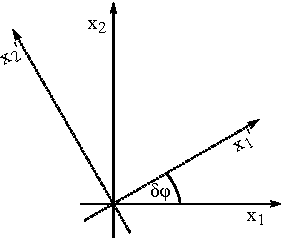
\includegraphics{283Drehung}
\end{center}
$\vv x \longrightarrow \vv x ' = R( \delta \phi) \vv x \stackrel{(265)}= \vv x - \delta \vv \phi \times \vv x$
\eqnnon{
\psi(\vv x) \longrightarrow \psi'(\vv x') & = \psi( \vv x) - \psi(\vv x' + \delta \vv \psi \times \vv x') + \mathcal O ( \delta \phi^2) \\
& = \psi( \vv x') + ( \delta \vv \phi \times \vv x') \cdot \vv \nabla \psi( \vv x') \\
& = \psi( \vv x') + ( \vv x' \times \vv \nabla \psi) \delta \vv \phi \\
& = \psi( \vv x') + \frac i \hbar \delta \vv \phi \cdot \vv x  \times P \psi ( \vv x') \\
& = \psi( \vv x ') + \frac i \hbar \delta \vv \phi \cdot \vv L \psi( \vv x')
}
mit
\eqn{ \vv L & = \vv X \times P \mathrm{ \quad Bahndrehimpuls}}
Endliche Drehung
\eqn{ \psi'( R( \vv \phi) \vv x) & = e^{\frac i \hbar \vv \phi \vv L} \psi( \vv x) }
bedeutet:
\eqn{ L_j & = \eps_{jkl} X_k P_l}
Mit $[X_k, P_l] = i \hbar \delta_{kl}$ findet man
\eqn{ [L_j, L_k] = i \hbar \eps_{jkl} L_l}
(Aufgabe 18), so dass $\frac{L_j}\hbar$ tats"achlich (279) erf"ullt.

Gesamtdrehimpuls
\eqn{ \vv J = \vv L + \vv S,}
wobei
\eqn{ [L_j, S_k ] & = 0, \\
[J_j, J_k] & = i \eps_{jkl} J_l}

\subsection{Eigenwerte des Drehimpulsoperator}
\eqn{
\begin{split}
\left[ \vv J ^2, J_k \right] & = \sum_{k=1}^3 \left[ J_k [J_k, J_m] +[J_k, J_m] J_k \right] \\
& \stackrel{(250)}= i \hbar \sum_{k,l=1}^3 \underbrace{ \eps_{kml}}_{\mathrm{antisym.}} \underbrace{ (J_k J_l + J_l J_k)}_{\mathrm{\ sym. \ bzgl. \ Austausch \ } \atop k \mathrm{ \ und \ } l} \\
& = 0 
\end{split}
}
$\leadsto$ Casimir-Operator

$\Longrightarrow$ gemeinsame Eigenkets von $\vv J^2$ und $J_3$
\eqn{
\begin{split}
\vv J^2 \Ket{ \lambda m} & = \lambda \hbar^2 \Ket{ \lambda m} \\
J_3 \Ket{ \lambda m} & = m \hbar \Ket{ \lambda m}
\end{split}
}
Es gilt
\eqn{\Braket{ \lambda m | \vv J^2 | \lambda m } \geq 0 \Longrightarrow \lambda \geq 0}
Leiteroperatoren: $J_\pm = J_1 \pm i J_2$, also \eqn{J_{\pm}^\dagger = J_{\mp}}

Dann:
\begin{aaufz}
\item $[J_3, J_{\pm}] = [J_3, J_1 ] \pm i [J_3, J_2] = (i J_2 \pm J_1) \hbar = \pm J_{\pm} \hbar$ \hfill (295)
\item $[J_+, J_-] = 2 J_3 \hbar$ \hfill (296)
\item $\vv J^2 = J_+ J_- + J_3^2 - J_3 \hbar = J_- J_+ + J_3^2 + J_3 \hbar$ \hfill (297) 
\item $[\vv J^2, J_{\pm}] = 0$ \hfill (298)
\end{aaufz}
\setcounter{equation}{298}
Wegen (298) ist $\vv J^2 J_{\pm} \Ket{ \lambda m} = J_{\pm} \vv J^2 \Ket{ \lambda m} = J_{\pm} \lambda \hbar \ket{\lambda m}$. $\Longrightarrow$ $J_\pm \ket{\lambda m }$ ist EZ zu $\vv J^2$ mit EW $\lambda \hbar^2$ oder $J_\pm \Ket {\lambda m} = 0$.
\eqn{
\begin{split}
J_3 J_\pm \Ket{\lambda m} & \stackrel{(285)}= J_{\pm} \underbrace{ J_3 \Ket{\lambda m}}_{\hbar m \Ket{\lambda m}} \pm  J_\pm \hbar \Ket{\lambda m} \\
& = (m \pm 1) \hbar J_\pm \Ket{\lambda m}
\end{split}
}
$\Longrightarrow$ $J_\pm \Ket{\lambda m}$ ist EZ zu $J_3$ mit EW $(m \pm 1) \hbar$ oder $J_\pm \Ket{\lambda m} = 0$.
\eqn{
\begin{split}
0 \leq \left\Vert J_pm \Ket{ \lambda m} \right\Vert^2 & = \Braket{ \lambda m | J_\mp J_\pm | \lambda m } \\
& \stackrel{(297)}= \braket{ \lambda m | \vv J^2 - J_3^2 \mp J_3 \hbar | \lambda m} 
\end{split}\\
& = \lambda - m^2 \mp m
}
$\Longrightarrow \lambda \geq m^2 \pm m$ $\Longrightarrow \lambda \geq \vert m \vert ( \vert m \vert + 1) \geq 0$ \hfill (302)
\setcounter{equation}{302}
$\Longrightarrow$ Es gibt f"ur jedes $\lambda$ ein maximalex $m$:
\eqn{j := m_{\mathrm{max}}}
$\Ket{\lambda j}$ hei"st \emph{Zustand h"ochsten Gewichts}:
\eqn{J_+ \Ket{\lambda j } = 0}
$\Longrightarrow$
\eqnnon{0 = \left\Vert J_+ \ket{ \lambda j } \right\Vert^2 \stackrel{(301)}= \lambda - j^2 - j}
$\Longrightarrow$
\eqn{ \lambda = j(j+1)}
Analog f"ur $m_{\mathrm{min}}$ und $J_- \Ket{ \lambda m_{\mathrm{min}}}$:
\eqn{
0 & = \lambda - m_{\mathrm{min}}^2 + m_{\mathrm{min}} \stackrel{(305)}= j(j+1) - m_{\mathrm{min}}^2 + m_{\mathrm{min}} \notag \\
\Longrightarrow m_{\mathrm{min}} &= - j
}
$m$ nimmt also die Werte
\eqn{-j, -j+1, \ldots j-1, j}
an. $\Longrightarrow$
\eqn{
\begin{split}
2j & \in \NN_0, \mathrm{ \ also} \\
j & =0, \frac12, 1, \frac32, 2, \ldots
\end{split}
}
Bessere Notation:
\eqn{
\spl{
\vv J^2 \Ket{jm} & = j(j+1) \hbar^2 \Ket{jm} \\
J_3 \Ket{jm} & = m \hbar \Ket{ j m }
}
}
und der Zustand h"ochsten Gewichts ist $\Ket{ jj}$.

Eigenwerte des Bahndrehimpuls:
$$ \vv L = \vv X \times \vv P \ \Longrightarrow \mathrm{Quantenzahlen \ } l, m_l$$
Spektrum gegenüber (308) weiter eingeschr"ankt.
\eqn{
a_j & := \frac1{\sqrt 2} \left[ \frac{X_j}{x_0} + i \frac{x_0 P_j}\hbar \right] \\
\spl{
a_+ &:= \frac1{\sqrt2} (a_1 + i a_2) \\
a_+^+ & := \frac1{\sqrt2} (a_1^+ - i a_2^+) \\
a_- & := \frac1{\sqrt2} (a_1 - i a_2) \\
a_-^+ & := \frac1{\sqrt2} (a_1^+  + i a_2^+)
}
}
(dabei ist $x_0$ beliebiger Parameter mit $[x_0] = $L"ange) erf"ullen (vgl (224))
\eqn{ [a_+, a_+^+] & = [a_-, a_-^+] = \dOne}
($\leadsto$ Auf- und Absteigeoperatoren) und
\eqn{ [a_+, a_-] = 0}
Weiter
\eqn{
\spl{
L_3 & \stackrel{(386)}= X_1 P_2 - X_2 P_1 \\
& \stackrel{(310)}= \frac \hbar {2i} \left[ (a_1 + a_1^+) (a_2 - a_2^+) - (a_2 + a_2^+) (a_1 - a_1^+) \right] \\
& = \frac \hbar i [a_1 ^+ a_2 - a_1 a_2^+] \\
& \stackrel{(311)}= \hbar [a_-^ + a_- - a_+^+ a_+ ] \\
& = \hbar (N_- - N_+)
}
}
mit Besetzungszahloperator $N_+$ und $N_-$.

(235) $\Longrightarrow$ EW von $N_\pm$ sind ganzzahlig

$\Longrightarrow$ $L_3$ hat nur ganzzahlige EW
\eqn{ m_l = -l, -l+1, \ldots, -1, 0, 1, \ldots l-1, l}
$\Longrightarrow$ Die Quantenzahl $l$ in der EW-Gleichung (vgl. (309))
\eqn{ \vv L^2 \Ket{ l m_l } & = \hbar^2 l(l+1) \Ket{ l m_l }}
ist ebenfalls ganzzahlig.

Normierung:
\eqn{ \mathrm{(300)} \Longrightarrow J_- \Ket{ jm } \propto \Ket{ j \, m-1}}
(301) $\wedge$ (305) $\Longrightarrow$ $\Vert J_- \Ket{j m} \Vert^2 = j(j+1) - m(m-1)$

W"ahle
\eqn{
\Ket{j \, m-1} & := \frac 1 {\sqrt{j(j+1) - m(m-1)}} J_- \Ket{ j \, m } \\
& \mathrm{"`Condor-Shortley-Phasenkonvention} \notag\\
\Ket{j \, m+1 } & := \frac 1 {\sqrt{j(j+1) - m(m+1)}} J_+ \Ket{ j \, m }
}
Analog
\eqn{ \Ket{ l \, m_l - 1} & := \frac 1 {\sqrt{l(l+1) - m_l(m_l-1)}} L_- \Ket{ l \, m_l }}
mit $L_\pm = L_1 \pm i L_2$.

Graphisch:
\begin{center}
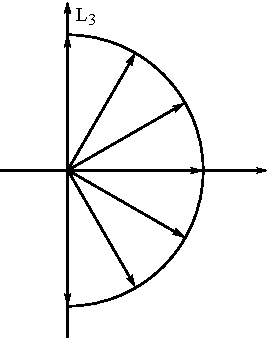
\includegraphics{320L3}
\end{center}
Ortsdarstellung: Polarkoordinaten $r, \vartheta, \phi$:
\eqn{ 
\spl{
\left[ \vv X^2, \vv L \right] & = \sum_{j=1}^3 \left[ X_j^2, \vv L \right] \\
& = \sum_{j=1}^3 \left\{ X_j [X_j, \vv L] + [X_j, \vv L] X_j \right\} \\
& \stackrel{(A18b)}=0
}}
Eigenfunktionen:
$$ \braket{ \vv r | l \, m } := \Braket{ r \, \vartheta \, \phi | l \, m }$$
($m$ steht f"ur $m_l$)
\eqn{
\spl{
\Braket{ \vv r | \vv L^2  | l \, m } & = \hbar l (l+1) \Braket{ \vv r| l \, m } \\
\Braket{ \vv r | L_3 | l \, m } & = \hbar m \Braket{ \vv r | l \, m }
}
}
In der Ortsdarstellung bedeutet (321):
$$[r^2, \vv L ] = 0,$$
d.h. $\vv L$ enth"alt keine Ableitungen nach $r$.

$\Longrightarrow$ Wir suchen nach Eigenfunktionen, die nicht von $r$ abh"angen: $\Braket{ \vv r | l \, m } = Y_{lm} ( \vartheta, \phi)$ \hfill (323)
\setcounter{equation}{323}
\eqn{ \spl{
\vv L^2 Y_{lm}(\vartheta, \phi) & = \hbar^2 l(l+1) Y_{lm}(\vartheta, \phi) \\
L_3 Y_{lm}(\vartheta, \phi) & = \hbar m Y_{lm}(\vartheta, \phi)
}}
wobei $L_j$ ein Differentialoperator bzgl. $\vartheta$ und $\phi$ ist. Mit $Y_{lm}( \vartheta, \phi)$ ist auch $f(r) Y_{lm}( \vartheta, \phi)$ mit beliebigen $f(r)$ eine L"osung von (324).
\eqn{ \vv \nabla & = \vv{e_r} \frac \partial {\partial r} + \vv{e_\vartheta} \frac1r \frac \partial {\partial \vartheta} + \vv{e_\phi} \frac1{r \sin \vartheta} \frac \partial {\partial \phi}}
mit $\vv x = r \vv{e_r}$, $\vv {e_r} \times \vv {e_\vartheta} = \vv{ e_\vartheta} = \vv{e_\phi}$ usw.
\eqn{
\spl{
\vv L & = \frac \hbar i \vv X \times \vv \nabla \\
& = \frac \hbar i \left[ \vv{ e_\phi} \frac \partial {\partial \vartheta} - \vv{e_\vartheta} \frac1{\sin \vartheta} \frac \partial {\partial \phi }\right] \\
& = \frac \hbar i \left[ \matr{ - \sin \phi \\ \cos \phi \\ 0 } \frac \partial {\partial \vartheta} + \matr{ - \cot \vartheta \cos \phi \\ - \cot \vartheta \sin \phi \\ 1 } \frac \partial {\partial \phi} \right]
}
}
$\Longrightarrow$
\eqn{ \vv L^2 & = - \hbar^2 \Delta_{\vartheta, \phi}}
wobei 
\eqn{ \Delta_{\vartheta, \phi} = \frac1{\sin \vartheta} \frac \partial {\partial \phi} \frac \partial {\partial \vartheta} \left( \sin \vartheta \frac \partial {\partial \vartheta} \right) + \frac1{\sin^2 \vartheta} \frac{\partial^2}{\partial \phi^2}}
Laplace-Operator in Kugelkoordinaten:
\eqn{ \Delta = \frac{\partial^2}{\partial r^2} + \frac2r \frac \partial {\partial r} + \frac1{r^2} \Delta_{vartheta, \phi}.}
(326) $\Longrightarrow$
$$L_3 = \frac \hbar i \frac \partial {\partial \phi}$$
(324) $\Longrightarrow$ 
$$\frac \hbar i \frac \partial {\partial \phi} Y_{lm}(\vartheta, \phi) = \hbar m Y_{lm} ( \vartheta, \phi)$$
$\Longrightarrow$
\eqn{Y_{lm} (\vartheta, \phi) & = e^{i m \phi} Y_{lm}(\vartheta, 0)}
Aus (326) finden wir
\eqn{ L_\pm = L_1 \pm i L_2 = h \exp \left\{\pm i \phi \left[ \pm \frac \partial{\partial \vartheta} + i \cot \vartheta \frac \partial {\partial \phi} \right] \right\}}
Aus $L_+ \Ket{ l  \, l } = 0$ folgt
\eqn{ \spl{
0 = L_+ Y_{ll}(\vartheta, \phi) & \stackrel{(331),(330)}= \hbar \exp \left\{ i \phi \left[ \frac \partial {\partial \vartheta} + i \cot \vartheta \frac \partial{\partial \phi} \right] \right\} Y_{ll}(\vartheta, \phi) \\
& = \exp \left\{ i (l+1) \phi \left( \frac \partial {\partial \vartheta} - l \cot \vartheta \right) \right\} Y_{ll} (\vartheta, 0)
}}
L"osungsweg wie (241) $\longrightarrow$ (242) $\Longrightarrow$
\eqn{ Y_{ll}( \vartheta, 0) = C_l (\sin \vartheta)^l }
Normierung:
\eqn{ 1 & = \int_0^\pi \dd \vartheta \, \sin \vartheta \int_0^{2\pi} \dd \phi \, \vert Y_{lm}(\vartheta, \phi) \vert^2 }
(333) $\Longrightarrow$
\eqn{ \vert C_l \vert^2 & = \frac{2l +1}{4 \pi} \frac1{?^l} \left( { 2l \atop l } \right)m \\
L_- Y_{lm}(\vartheta, \phi) & \stackrel{(320)}= \sqrt{ l(l+1) - m(m-1)} \hbar Y_{l, m-1} (\vartheta, \phi)
}
Mit (330) und (331):
$$a_{lm} \exp\left\{i(n-1) \phi \right\} Y_{l, m-1}(\vartheta, 0) = \exp \left\{ - i \phi \left[ - \frac \partial {\partial \vartheta} + i \cot \vartheta \frac \partial {\partial \phi} \right] \right\} Y_{lm}(\vartheta, 0)$$
$\Longrightarrow$
$$a_{lm} Y_{l, m-1} (\vartheta, 0) = \left[ - \frac \partial {\partial \vartheta} - m \cot \vartheta \right] Y_{lm}(\vartheta, 0)$$
Standardtrick:
\eqn{ \spl{ a_{lm} Y_{l, m-1} (\vartheta, 0) & = \left[ - \frac \partial {\partial \vartheta} + m \cot \vartheta \right] (\sin \vartheta)^{-m} \sin^m Y_{lm}(\vartheta, 0) \\
& = -(\sin \vartheta)^{-m} \frac \partial {\partial \vartheta} ( \sin \vartheta)^m Y_{lm}(\vartheta, 0),
}}
denn
$$\frac \partial {\partial \vartheta} (\sin \vartheta)^{-m} = -m (\sin \vartheta)^{-m-1} \cos \vartheta = -m (\sin \vartheta)^{-m} \cot \vartheta$$
also
$$\left[ \frac \partial{\partial \vartheta} + m \cot \vartheta \right] (\sin \vartheta)^{-m} = 0.$$
Mit $t:= \cot \vartheta, \ \sin^2 \vartheta = 1 - t^2$ ist
$$\frac \partial {\partial \vartheta} = \frac {dt}{d\vartheta} \frac d{dt} = - \sin \vartheta \frac d {dt}$$
und (337) ist
\eqnnon{
a_{lm} Y_{l, m-1} (\vartheta, 0) & = (\sin \vartheta)^{-(m+1)} \frac d{dt} (\sin \vartheta)^m Y_{lm} (\vartheta, 0) \\
& = (1- t^2)^{-\frac{n-1}2} \frac d{dt} (1-t^2)^{\frac n2} Y_{lm}(\vartheta, 0)
}
$\Longrightarrow$ Rekursionsformel:
\eqn{\underbrace{ (1-t^2)^{\frac{n-1}2} Y_{l, m-1}}_{f_{l, m-1}(t) = \frac 1{a_{lm}} \frac d{dt}} & = \frac 1{a_{lm}} \frac d{dt} \underbrace{ \left[ (1-t^2)^{\frac m2} Y_{lm}(\vartheta,0) \right]}_{f_{lm(t)}}}
Anfangsbedingung $m=l$ aus (333):
\eqn{
Y_{ll}(\vartheta, 0) & = C_l (1-t^2)^{\frac l 2} \notag \\
\Longrightarrow f_ll(t) & = (1-t^2)^{\frac l2} Y_{ll}(\vartheta, 0) = C_l (1-t^2)^l
}
L"osung von (338)
\eqn{
f_{l,l-1}(t) & = \frac1{a_{ll}} \frac d{dt} f_{ll}(t),  \\
f_{l,l-2}(t) & \stackrel{(332)}= \frac1{a_{l,l-1}} \frac d{dt} f_{l, l-1}(t) \notag \\
& \stackrel{(340)}= \frac1{a_{l,l-1}} \frac 1{a_ll} \frac{d^2}{dt^2} f_{ll}(t), \notag \\
f_{lm}(t) & = \frac1{a_{ll} \cdots a_{l,m+1}} \frac{d^{l-m}}{dt^{l-m}} f_{ll}(t) \notag
}
(338), (339) $\Longrightarrow$
$$Y_{lm}(\vartheta, 0) = \frac{C_l}{a_{ll} \cdots a_{l, m-1}} (1-t^2)^{- \frac m2 } \frac{d^{l-m}}{dt^{l-m}} (1-t^2)^l$$
Die L"osung schreibt man "ublicherweise als
\eqn{Y_{lm}(\vartheta, 0) & = C_{lm} P_l^m(t)}
mit
\eqn{C_{lm} & = (-1)^m \left[ \frac{2l + 1}{4 \pi} \frac{ (l-m)!}{(l+m)!} \right]^{\nicefrac 12}}
und den \emph{zugeordneten Legendre-Funktionen}
\eqn{P_l^m(t) & = (-1)^{l +m} \frac{(l+m)!}{(l-m)!} \frac1{2^l l!} (1-t^2)^{-\frac n2} \frac{d^{l-m}}{dt^{l-m}} (1-t^2)^l}
Eigenschaften:
\eqn{P_l^{-m}(t) & = (-1)^m \frac{(l-m)!}{(l+m)!} P_l^m(t)}
also (via $m \longrightarrow -m$ in (343)):
\eqn{P_l^m(t) & = \frac1{2^l l!} (1-t^2)^{\frac n2} \left( \frac d{dt} \right)^{l+m} (t^2 - 1)^l }
Die 
\eqn{Y_{lm}(\vartheta, \phi) = C_{lm} P_l^m (\cos \vartheta )e^{i m \phi}}
hei"sen \emph{Kugelfl"achenfunktionen}. Es gilt
\eqn{ Y_{lm}(\vartheta, \phi) & = (-1)^m Y_{lm}^* (\vartheta, \phi)}

\begin{center}
\begin{tabular}{l l }
Physik & Chemie \\
\hline 
$Y_{00} = \frac1{\sqrt{4\pi}}$ & s-Orbital \\
\hline
$Y_{11} = -\sqrt{ \frac 3{8 \pi}} \sin \vartheta e^{i \phi}$ & \multirow{3}{*}{p-Orbitale} \\
$Y_{10} = \sqrt{ \frac 3 {4\pi}} \cos \vartheta$ \\
$Y_{1-1} = -Y_{11}^* = \sin \vartheta e^{- i \phi}$ \\
\hline
$Y_{22} = \sqrt{ \frac {15}{32 \pi}} \sin^2 \vartheta e^{i \phi}$ & \multirow{5}{*}{d-Orbitale} \\
$Y_{21} = -\sqrt{ \frac{15}{8 \pi}} \sin \vartheta \cos \vartheta e^{i \phi}$ \\
$Y_{20} = \sqrt{\frac5{16 \pi}} (3 \cos^2 \vartheta - 1)$ \\
$Y_{2,- 1} = - Y_{21}^*$ \\
$Y_{2, -2} = - Y_{22}^*$
\end{tabular}
\end{center}
Normierung: $\Braket{ l' \, m' | l \, m} = \delta_{l l'} \delta_{m m '}$ $\Longrightarrow$
\eqn{\int \dd \Omega \, Y_{l' m'}^* (\vartheta, \phi) Y_{l m}(\vartheta, \phi) = \delta_{l l'} \delta_{m m '}}
Vollst"andigkeit: $\dOne = \sum_{l=0}^\infty \sum_{m=-l}^l \Ket{ l \, m} \Bra{l \ m}$ $\Longrightarrow$
\eqn{\sum_{l=0}^\infty \sum_{m=-l}^l Y_{lm}^*(\vartheta, \phi) Y_{lm} (\vartheta', \phi') = \delta( \Omega - \Omega') = \frac{ \delta(\vartheta - \vartheta') \delta(\phi - \phi')}{\sin \vartheta}}
$\vert Y_{lm}(\vartheta, \phi) \vert^2 \dd \Omega$ ist die Aufenthaltswahrscheinlichkeit im Raumwinkelelement $\dd \Omega$ um $(\vartheta, \phi)$ f"ur Elektron mit Drehimpuls $-QZ(l,n)$

\psset{xunit=50pt}
\psset{yunit=50pt}

\begin{center}
\begin{longtable}{c c}
$l=0$, $m=0$: & $l=1$, $m=1$: \\  
\begin{pspicture}(-1.5,-1.5)(1.5,1.5)
\parametricplot[plotstyle=curve,  plotpoints=1000]{0}{360}{t sin t cos}
\end{pspicture} 
&
\begin{pspicture}(-1.5,-1.5)(1.5,1.5)
\parametricplot[plotstyle=curve,  plotpoints=1000]{0}{360}{t sin 2 exp t sin mul 1.5 mul t sin 2 exp t cos mul 1.5 mul}
\end{pspicture}
\\
\newpage
$l=1$, $m=0$: & $l=2$, $m=2$: \\
\begin{pspicture}(-1.5,-2)(1.5,2)
\parametricplot[plotstyle=curve, plotpoints=1000]{0}{360}{t cos 2 exp t sin mul 1.5 mul t cos 2 exp t cos mul 1.5 mul}
\end{pspicture}
&
\begin{pspicture}(-1.5,-2)(1.5,2)
\parametricplot[plotstyle=curve, plotpoints=1000]{0}{360}{t sin 4 exp t sin mul 1.6 mul t sin 4 exp t cos mul 1.6 mul}
\end{pspicture}
\\
$l=2$, $m=1$: & $l=2$, $m=0$: \\
\begin{pspicture}(-1.5,-2.5)(1.5,2.5)
\parametricplot[plotstyle=curve, plotpoints=1000]{0}{360}{t sin t cos mul 2 exp t sin mul 7.5 mul  t sin t cos mul 2 exp t cos mul 7.5 mul}
\end{pspicture}
&
\begin{pspicture}(-1.5,-2.5)(1.5,2.5)
\parametricplot[plotstyle=curve, plotpoints=1000]{0}{360}{t cos 2 exp 3 mul 1 sub 2 exp t sin mul 0.5 mul t cos 2 exp 3 mul 1 sub 2 exp t cos mul 0.5 mul }
\end{pspicture}
\end{longtable}

\end{center}

Parit"at:
$$\mathcal P: \psi( \vv r) \longmapsto \psi(- \vv r)$$
F"ur $\psi( \vv r) = f(r) Y_{lm} (\vartheta, \phi)$ ist
$\psi(- \vv r) = f(r) Y_{lm} (\pi - \vartheta, \phi + \pi)$

Aus (346) und (343):
\eqn{ Y_{lm}(\pi - \vartheta, \phi + \pi) = (-1)^l Y_{lm}(\vartheta, \phi)}
$\Longrightarrow$ Die Parit"at von $Y_{lm}$ ist $(-1)^l$.


\section{Wasserstoffatom}

\subsection{Zentralpotentiale}

\eqn{V(\vv X) = V(R)}
mit $R^2 = X_1^2 + X_2^2 + X_3^2$ und $V(R) = V(r) = V(\sqrt{\vv x^2})$ in der Ortsdarstellung.

In beliebiger Darstellung:
$$V(R) = \int_{\RR^3} \dd \vv x \, \Ket{\vv x} V\left(\sqrt{ \vv X^2}\right) \Bra{\vv x}$$
Rotationsinvarianz:
$$e^{\frac i \hbar \vv \phi \vv J} V(R) e^{- \frac i \hbar \vv \phi \vv J} = V(R)$$
Infinitesimal:
$$\left[ 1 + \frac i \hbar \vv \phi \vv J \right] V(R) \left[1 - \frac i \hbar \vv \phi \right] = V(R) + \mathcal O(\phi^2)$$
$\Longrightarrow$
\eqn{ \left[ \vv J , V(R) \right] = 0.}
Auch
\eqn{ \left[ J, \vv P^2 \right] = 0, }
also 
\eqn{ \left[ J, H \right] = 0 }
Energieeigenkets:
\eqn{\Ket{ E \, j \, m}}
Ist $V(R)$ zus"atzlich auch von $\vv S$ unabh"angig (?), so ist $[S, V(R)] = 0$, also auch (wegen $\vv L = \vv J - \vv S$)
$$\left[ \vv L, V(R) \right] = 0$$
So k"onnen wir die Energieeigenkets mit
\eqn{ \Ket{E \, l \, m_l \, s \, m_s } }
bezeichnen.

(354) $\Longrightarrow$ $[H, J_\pm] = 0$. Aus $H \Ket{ E \, j \, m} = E \Ket{ E \, j \, m }$ folgt also
$$H J_\pm \Ket{E \, j \, m} = J_\pm H \Ket{E \, j \, m} = E J_\pm \Ket{ E \, j \ , m }$$
$\Longrightarrow$
$$H \Ket{E \, j \, m \pm 1} = E \Ket{ E \, j \, m\pm 1}$$
$\Longrightarrow$ $E$ h"angt nicht von $m$ ab.

Zun"achst $[\vv S, V(R)] = 0$
\eqn{ \spl{ H & = \frac{P^2}{2m} + V(R), \\ \Ket{ E \, l \, m_l \, s \, m_s } & = \Ket{ E \, l \, m_l } \otimes \Ket{ s \, m_s}}}
Spin-Entartung: $E$ h"angt nicht von $m_s = \pm \frac12$ ab.
$$H \Ket{E \, l \, m_l } = E \Ket{ E \, l \, m_l }$$
mit $\psi_{E l m_l}(\vv r) = \Braket{ \vv r | E \, l \, m_l }$
$\Longrightarrow$
\eqn{ \left[ - \frac{\hbar^2}{2m} \Delta + V(r) \right] \psi_{E l m_l}(\vv r) & = E \psi_{E l m_l}(\vv r)}
bzw. mit (327), (329):
\eqn{ P^2 = - \hbar^2 \Delta & = P_r^2 + \frac1{r^2} \vv L^2}
wobei
\eqn{P_r^2 & = -\hbar^2 \left[ \frac {\partial^2}{\partial r^2} + \frac2r \frac \partial {\partial r} \right]. }
Radialimpuls
\eqn{ P_r & = \frac \hbar i \left( \frac \partial {\partial r} + \frac1r \right) }
erf"ullt
\eqn{ \spl{ P_r^\dagger & = P_r, \\ \left[ P_r, R \right] & = \frac \hbar i \dOne }}
(358) bedeutet also
\eqn{ \left[ \frac1{2m} P_r^2 + \frac1{2mr^2} \vv L^2 + V(r) \right] \psi_{E l m_l }(\vv r) & = E \psi_{E l m_l }(\vv r)}
Mit 
\eqn{ \vv L^2 \psi_{E l m_l} (\vv r) & = \hbar^2 l (l+1) \psi_{E l m_l}(\vv r)}
folgt (siehe Text (324)):
\eqn{\psi_{E l m_l}(\vv r) & = f_{E l}(r) Y_{l m_l}( \vartheta, \phi) }
und (363) wird zu 
$$\left[ \frac 1{2m} P_r^2 + \frac{\hbar^2 l (l+1)}{2 m r^2} + V(r) \right] f_{E l} (r) Y_{l m_l} ( \vartheta, \phi)  = E f_{El}(r) Y_{l m_l}(\vartheta, \phi)$$
Und mit (360):
\eqn{\left[ - \frac{\hbar^2}{2m} \left( \frac{\partial^2}{\partial r^2} + \frac 2 r \frac \partial {\partial r} \right) + \frac{ \hbar^2 l (l+1) }{2 m r^2} + V(r) \right] f_{E l}(r) & = E f_{E l}(r)}
$\Longrightarrow$ tats"achlich keine $m_l$-Abh"angigkeit.

In (366) o.B.d.A. $f_{E l }(r)$ reell:

Trick: $U_{E l}(r) := r f_{E l}(r)$, dann
\eqnnon{
\frac{\partial^2}{\partial r^2} U_{E l}(r) & = \frac{ \partial}{\partial r} \Big[ \underbrace{ \left( \frac{\partial r}{\partial r} \right)}_{=1} f_{E l}(r) + r \frac{\partial}{\partial r} f_{E l}(r) \Big] \\
& = 2 \frac{\partial}{\partial r} f_{E l}(r) + r\frac{\partial^2}{\partial r^2} f_{E l}(r) \\
& = r \left[ \frac{\partial^2}{\partial r^2} + \frac2r \frac \partial {\partial r} \right] f_{E l}(r)
}
und (366) wird zu 
\eqn{ \left[ - \frac{\hbar^2}{2m} \frac{\partial^2}{\partial r^2} + \frac{\hbar^2 l(l+1)}{2m r^2} + V(r) \right] U_{E l} (r) & = E U_{E l}(r).}
Das entspricht 1-dim Schr"odinger-Gleichung mit
\eqn{ V_{\mathrm{Eff}}(r) = V(r) + \underbrace{ \frac{\hbar^2 l(l+1) }{2m r^2}}_{\mathrm{Zentrifugalpotenzial}}}
Jedoch $r \geq 0$. $\dd^3 \vv r = r^2 \dd r \dd \Omega$.

Bindungszust"ande:
$$\infty > \int_0^\infty r^2 \dd r \, f_{E l}^2 (r) = \int_0^\infty \dd r\, U_{E l}^2(r)$$
$\Longrightarrow$
\eqn{ \vert U_{El}(r) \vert \sqrt r \longrightarrow 0 \ \mathrm{f"ur \ } r \longrightarrow \infty}
Nun $r \longrightarrow 0$:

Zwei F"alle:
\begin{1aufz}
\item $U(0) \neq 0$ $\Longrightarrow$ $f(r) \stackrel{r \rightarrow 0}\sim \frac1r$ $\Longrightarrow$
$$\left[ - \frac{\hbar^2}{2m} \Delta + V(r) \right] f(r) Y_{l m_l} (\vartheta, \phi) \stackrel{r \rightarrow 0}\sim \left[ - \frac{\hbar^2}{2m} \delta^{(3)}(\vv r) + V(r) \frac1r \right] Y_{l m_l} (\vartheta, \phi) $$
$\Longrightarrow$ $V(r)$ hat $\delta^{(3)}(\vv r)$-singul"aren Anteil.
\item $U_{E l}(0) = 0$ $\Longrightarrow$ $V(r)$ hat keinen $\delta^{(3)}(\vv r)$-singul"aren Anteil
\end{1aufz}
F"ur die Meisten Potenziale gilt
$$r^2 V(r) \longrightarrow 0 \ \mathrm{f"ur \ } r \longrightarrow 0,$$
so dass $V_{\mathrm{eff}}(r)$ in (368) f"ur $r \longrightarrow 0$ vom Zentrifugalpotenzial dominiert ist, sofern $l \neq 0$.

$$r \longrightarrow 0: \quad \frac{d^2 U_{E l}}{d r^2} - \frac{l(l+1)}{r^2} U_{E l} = 0$$
regul"are L"osung:
\eqn{U_{E l}(r) \stackrel{r \rightarrow \infty}\sim r^{l+1} \ \mathrm{f"ur \ } l \neq 0}
irregul"are L"osung:
$$U_{E l}(r) \sim r^{-l}$$
im Widerspruch zu $U_{E l}(0) = 0$.

\subsection{Wasserstoffatom}

Es gilt $m_p = 1800 m_e$. $\leadsto$
\eqn{ V(r) = - \frac \gamma r}
mit 
\eqn{\gamma = \underbrace{ \frac{e^2}{4 \pi \eps_0}}_{\mathrm{SI- \atop Einheiten}} = \underbrace{h c \alpha}_{\mathrm{in \ jedem \atop Einheitensystem}}}
$\alpha \approx \frac 1 {137}$ hei"st Sommerfeld'sche Feinstrukturkonstante.

\emph{Bindungszust"ande}: $E < 0$:

Welllenfunktion:
\eqn{ \spl{ \psi_{E l m_l}(\vv r) & \stackrel{(365), (367)}= f_{E l}(r) Y_{l m_l} (\vartheta, \phi) \\
& = r U_{E l}(r) Y_{lm}(\vartheta, \phi)}}
Die Radialgleichung in (367) wird mit
\eqn{ \spl{
\rho & = \kappa r, \\
\kappa^2 & = \frac{2m \vert E \vert}{\hbar^2}, \ \kappa > 0, \\
\rho_0 & = \frac{2m \gamma}{\hbar^2 \kappa}}}
zu 
\eqn{ \left[ - \frac{d^2}{d \rho^2} - \frac{l(l+1)}{\rho^2} + \frac{\rho_0}\rho - 1 \right] U_{E l} (\rho) = 0}
Asymptotik: $U_{E l}(rho) \stackrel{\rho \rightarrow 0}\sim \rho^{l+1}$, siehe (370).

F"ur $\rho \rightarrow \infty$ wird (375) zu 
$$\frac{d^2 U_{E l}(\rho)}{d \rho^2} - U_{El}(\rho) = 0$$
$\Longrightarrow$
\eqn{ U_{E l}(\rho) \stackrel{\rho \rightarrow \infty}\sim e^{- \rho}}
Ansatz: 
\eqn{U(\rho) = \rho^{l+1} e^{-\rho} W(\rho)}
Einsetzen in (315):
\eqn{ \rho W''(\rho) + 2(l+1-\rho) W(\rho) + \left[ \rho_0 - 2(l+1) \right] W(\rho) = 0}
L"osung mit Potenzreihenansatz:
\eqn{W(\rho) = \sum_{k=0}^\infty a_k \rho^k}
Ideal f"ur Potenzreihenansatz:
\eqn{ \theta = \rho \frac d{d\rho},}
denn $\theta \rho^k = k \rho^k$ (gleiche Potenz)
\eqn{\rho^2 \frac{d^2}{d\rho^2} = \theta (\theta -1) = \theta^2 - \theta}
(378) wird zu
$$\left[ \theta (\theta-1) + 2(l +1 - \rho) \theta + (\rho_0 - 2(l+1)) \rho \right] W(\rho) = 0$$
Einsatzen von (349(:
\eqn{ \sum_{k=0}^\infty a_k \rho^k \left[ k(k-1) + 2(l+1-\rho) k + (\rho_0 - 2(l+1) \rho) \right] = 0}
Koeffizienten von $\rho^{k+1}$:
\eqn{ \left[ (k+1) k + 2(l+1) (k+1) \right] a_{k+1} + \left[ -2k + \rho_0 - 2(l+1) \right] a_k = 0 \mathrm{ \ f"ur \ } k \geq 0}
Der Koeffizient von $\rho^0$ in (382) ist $0$ $\Longrightarrow$ $a_0$  beliebig.

(383) $\Longrightarrow$
\eqn{a_{k+1} = \frac{2 (k+l+1) - \rho_0}{(k+1)(k+2l + 2)} a_k}
Noch mehr Asymptotik:

Entweder die Reihe bricht ab, oder (384) bedeutet
$$\frac{ a_{k+1}}{a_K} \stackrel{k \rightarrow \infty}\sim \frac 2k$$
also $a_k \stackrel{k \rightarrow \infty}\sim \frac{2^k}{k!}$. $\Longrightarrow$
$$W \stackrel{\rho \rightarrow \infty}\sim e^{2 \rho}$$
Widerspruch zu (376).

$\Longrightarrow$ Die Reihe muss abbrechen!

(384) $\Longrightarrow$ Es gibt ein $N \in \NN_0$ mit
\eqn{\rho_0 = 2(N+l+1),}
so dass in (384) $a_{N+1} = 0$ und 
\eqn{W(\rho) = \sum_{k=0}^N a_k \rho^k.}
Die Hauptquantenzahl $n = N+l+1$ erf"ullt wegen $N \geq 0, l \geq 0, \ N, l \in \NN_0$:
\eqn{n \in \NN.}
Also wegen (385) 
\eqn{\rho_0 = 2n.}
(374) $\Longrightarrow$
$$E = \frac{2 m \gamma^2}{\hbar^2 \rho_0}$$
Mit (388) sind die Eigenwerte durch die \emph{Balmerformel}
\eqn{E_n = - \frac{m \gamma^2}{2 \hbar n^2}, \quad n=1,2,3,\ldots}
gegeben.

(372) $\Longrightarrow$ 
\eqn{
& \mathrm{SI-System:} & E_n & = -\frac{me^4}{2 (4 \pi \eps_0)^2 \hbar^2} \frac1{\hbar^2} \notag \\
& \mathrm{jedes \ System:} & E_N & = - \frac{mc^2}2 \frac{\alpha^2}{n^2}
}
Statt $\Ket{ E \, l \, m_l}$ schreibt man $\Ket{ n \, l \, m}$. Wegen (385), (387) ist
\eqn{l \leq n -1.}
$l$ hei"st auch \emph{Nebenquantenzahl} und $m_l$ (was $\vert m_l \vert \leq l$ erf"ullt) \emph{magnetische QZ}.

Speziell f"urs Coulomb-Potenzial $V(r) = - \frac \gamma r$: $E_n$ h"angt nicht von $l$ ab.

Ursache: Runge-Lenz-Vektor ist Erhaltungsgr"o"se.

Die DGL (378) lautet in der Variablen $t = 2 \rho$:
\eqn{t \frac{d^2W}{dt^2} + \left[ 2l +1 +1 - t \right] \frac{dW}{dt} + \left[ n + l - (2l+1) \right] W & = 0}
(392) hei"st \emph{Laguerre'sche DGL}.
Die L"osungen
\eqn{W(\frac t2) = L_{n+l}^{2l +1}(t)}
hei"sen zugeordnete Laguerre-Polynome.

Es gilt:
\eqn{L_r^s(t)  &= \left( - \frac d{dt} \right)^2 e^t \left( \frac d{dt} \right)^r e^{-t} e^r,}
explizit:
\eqn{ \spl{
L_1^1(t) & = - \frac d{dt} e^t \left[ - e^{-t}t + e^{-t} \right] = 1 \\
L_2^1 (t) & = \frac 12 t^2 - 3t + 3 \\
L_3^3(t) & = - \frac{t^3}6 + 3t^2 - 15 t + 20
}}
Die Radialfunktionen $f_{E l}(r)$ in $(373)$ ist also mit (377) und (393):
\eqn{f_{n l }(r) = f_{E_nl}(r) = N_{nl}(2 \kappa r)^l e^{- \kappa r} L_{n+l}^{2l +1} (2 \kappa r)}
Normierungsfaktor:
\eqn{ N_{nl}^2 \frac{(n-l-1)!(2 \kappa^3)}{2n \left[ (n+l)! \right]^3}}
$\kappa$ h"angt von $n$ ab:
\eqn{\kappa = \frac{m \gamma}{\hbar n} = \frac 1{a n}}
mit dem Bohr'schen Radius:
\eqn{a = \frac{\hbar^2}{m \gamma} = \frac{ \hbar^2}{mc\alpha} \approx 0,529 \cdot 10^{-10} \meter}

Nullstellen:
\eqn{ 
&0: & f_{10}(r) & = 2a^{- \nicefrac 3 2} e^{- \nicefrac r a} \notag\\
&1:& f_{20}(r) & = 2 (2a)^{- \nicefrac 32} \left( 1 - \frac r{2a} \right) e^{- \frac r{2a}} \\
&2:& f_{21}(r) & = \frac 1{\sqrt 3} (2a)^{-\nicefrac 32} \frac r a e^{- \frac r {2a}} \notag}

Anzahl der Knoten: $N=n-l-1$ ("`radiale QZ"'). 

Die Wahrscheinlichkeit, das Elektron zwischen $r$ und $r+ \dd r$ anzufinden ist $p(r) \dd r$ mit
$$p(r) = r^2 f_{nl}^2(r).$$

\psset{xunit=30pt}
\psset{yunit=200pt}
\begin{center}
\begin{pspicture}*(0,0)(10,0.6)
\psplot[plotpoints=100, linecolor=red]{0}{10}{4 2.65 0 2 x mul sub exp mul x 2 exp mul}
\psplot[plotpoints=100, linecolor=blue]{0}{10}{4 0.125 mul 1 x 2 div sub 2 exp mul 2.65 0 x sub exp mul x 2 exp mul}
\psplot[plotpoints=100, linecolor=green]{0}{10}{0.333 1.125 mul x mul 2.65 0 x sub exp mul }
\psgrid[subgridwidth=0pt](0,0)(10,0.5)
\red \uput[r](6,0.5){$n=1, l=0$}
\blue \uput[r](6,0.4){$n=2, l=0$}
\green \uput[r](6,0.3){$n=2, l=1$}
\end{pspicture}
\end{center}
gr"o"seres $n$ $\Longrightarrow$ gr"o"seres $\Braket R$
\eqn{ \spl{ \Braket{r}_{nl} & := \Braket{ n \, l \ , m | R | n \, l \, m} \\
& = \int_0^\infty r^3 \dd r \, f_{nl}^3 (r) \\
& = \frac a 2 \left[ 3 n^2 - l(l+1) \right]
}}

\section{Zeitunabh"angige St"orungstheorie}

\subsection{Nicht entartete St"orungstheorie}

\eqn{H = H_0 + H_1}
Gel"ost:
\eqn{H_0 \Ket{n^{(0)}} = E_n^{(0)} \Ket{ n^{(0)}}}
Gesucht:
\eqn{ H\Ket n = E_n \Ket n}
$H_1$ sei klein gegen $H_0$, genauer:
\eqn{\Braket{ m^{(0)} | H_1 | n^{(0)} } \ll \vert E_n^{(0)} - E_m^{(0)}.}
insbesondere, Nichtentartung von $\Ket N$, d.h. $E_m^{(0)} \neq E_n^{(0)}$ f"ur $n \neq m$ und $\Ket n$ ist Bindungszustand.

\emph{St"orungstheorie:} L"osen von (404) durch Entwickeln in 
$$\frac{ \Braket{ m^{(0)} | H_1 | n^{(0)}} }{\left\vert E_n^{(0)} - E_m^{(0)} \right\vert}$$
Zweckm"a"sig: reeller Parameter $\lambda$ und
\eqn{H = H_0 + \lambda H_1 }
$\leadsto$ Organisation der St"orungstheorie in Potenzen von $\lambda$. 

St"orungsreihe:
\eqn{ \spl{ E_n & = E_n^{(0)} + \lambda E_n^{(1)} + \lambda^2 E_n^{(2)} + \ldots \\
\ket n & = \ket{ n^{(0)}} + \lambda \ket{ n^{(1)}} + \lambda^2 \ket{n^{(2)}} + \ldots }}
$\Ket n$ ist unnormiert: I.a. $\braket {n | n } \neq 1$.

(407) ist Potenzreihenansatz f"ur (404)
\eqn{ ( H_0 + \lambda H_1) \left( \ket{ n^{(0)}} + \lambda \ket{n^{(1)}} + \ldots \right) = (E_n^{(0)} + E_n^{(1)} + \ldots )\left(\ket n^{(0)} + \lambda \ket{n^{(1)}} + \ldots \right) }
Wir l"osen (408) f"ur alle $\lambda$
\eqn{ 
\lambda^0 & & H_0 \ket{ n^{(0)}} & = E_n^{(0)} \mathrm{, \ also (403} \notag\\
\lambda^1 & & H_1 \ket{ n^{(0)}} + H_0 \ket{n^{(1)}} & = E_n^{(1)} \ket{n^{(1)}} + E_n^{(0)} \ket{ n^{(0)}} \\
\lambda^2 & & H_1 \ket{ n^{(1)}} + H_0 \ket{n^{(2)}} & = E_n^{(2)} \ket{ n^{(2)}} + E_n^{(1)} \ket{n^{(1)}} + E_n^{(0)} \ket{ n^{(2)}}}
}
Entwickeln nach ungest"orten EZ:
\eqn{\ket{n^{(1)}} = \sum_k \ket{ k^{(0)}} \Braket{ k^{(0)} | n^{(1)}} \mathrm{, \ usw}}
Zur Bestimmung der Entwicklungskoeffizienten $\Braket{ k^{(0)} | n^{(1)}}$ und von $E_n^{(1)}$ multiplizieren wir (409) mit $\ket{ k^{(0)}}$:
\eqn{ \Braket{ k^{(0)} | H_1 | n^{(0)}} + \underbrace{ k^{(0)} | H_0 | n^{(1)}}_{E_k^{(0)} \Braket{ k^{(0)} | n^{(0)}}} & = E_n^{(1)} \underbrace{ \Braket{ k^{(0)} | n^{(0)}} }_{\delta_{kn}} + E_n^{(0)} \Braket{ k^{(0)} | n^{(1)}}}
F"ur $k=n$ liefer (412) die erste Korrektur zu Energie:
\eqn{ E_n^{(1)} & = \Braket{ n^{(0)} | H_1 | n^{(0)}}}
F"ur $k \neq n$ folgt aus (412):
\eqn{ \Braket{ k^{(0)} | n^{(1)}} = \frac{ \Braket{ k^{(0)} | H_1 | n^{(0)}} }{E_n^{(0)} -E_k^{(0)}}}
Jedoch $\braket{ n^{(0)} | n^{(0)}}$ ist unbestimmt!

Wir w"ahlen
\eqn{ \Braket{ n^{(0)} | n^{(1)}} = 0}
Also mit (411):
\eqn{\Ket{ n^{(1)}} = \sum_{k \neq n} \ket{ k^{(0)}} \frac{ \Braket{k^{(0)} | H_1 | n^{(0)}}}{E_n^{(0)} - E_k^{(0)}}}
($E_k^{(0)} \neq E_n^{(0)}$ f"ur $k \neq n$; f"ur $k \neq k'$ ist aber $E_k^{(0)} = E_{k'}^{(0)}$ erlaubt, solange $k, k' \neq n$)

In h"oheren Ordnungen k"onnen wir auch
\eqn{ \Braket{ n^{(0)} | n^{(k)}} = 0, \ k \geq 1}
fordern, denn zu jeder L"osung $\ket{ n^{(k)}}$ von (408) ist auch $\ket{ n^{(k)}} = \ket{n^{(k)'}} + \alpha \ket{ n^{(0)}}$ L"osung von (408) zur Ordnung $\lambda^k$.
$$0 = \Braket{ n^{(0)} | n^{(k)}} = \Braket{ n^{(0)} | n^{(k)'}} + \alpha \Braket{ n^{(0)} | n^{(0)}}$$
$\Longrightarrow$
$$\alpha  = - \Braket{ n^{(0)} | n^{(k)'}}$$
Aus (410) finden wir dann:
$$\Braket{ n^{(0)} | H_1 | n^{(1)}} + \underbrace{ \Braket{ n^{(0)} | H_0 | n^{(2)}}}_{E_n^{(0)} \underbrace{ \Braket{ n^{(0)} | n^{(2)}}}_{=0}} = E_n^{(2)} \underbrace{ \Braket{ n^{(0)} | n^{(0)}}}_{=1}$$
$\Longrightarrow$
\eqn{ \spl{
E_n^{(2)} & = \Braket{ n^{(0)} | H_1 | n^{(1)}} \\
& \stackrel{(416)}= \sum_{k \neq n} \frac{ \Braket{ n^{(0)} | H_1 | k^{(0)}} \Braket{ k^{(0)} | H_1 | n^{(0)}}}{E_n^{(0)} - E_k^{(0)}} \\
& = \sum_{k \neq n} \frac{ \left\vert \Braket{ k^{(0)} | H_1 | n^{(0)}} \right\vert^2}{E_n^{(0)} - E_k^{(0)}}
}}
Intepretation: W"ahrscheinlichkeit, ein im Zustand $\ket{n {(0)}}$ pr"apariertes System nach Einschalten im Zustand $\ket{ k^{(0)}} \neq \ket{n^{(0)}}$ anzutreffen:
\eqn{\spl{
P_{n \rightarrow k^{(0)}} & = \frac{ \left\vert \Braket{ k^{(0)} | n } \right\vert^2}{ \left\vert \Braket{n | n} \right\vert^2 } \\
& = \frac{ \left\vert \Braket{ k^{(0)} | n } \right\vert^2}{\left\vert 1 + \mathcal O(\lambda^2) \right\vert^2} \\
& \stackrel{(416)}= \frac{ \left\vert \Braket{ k^{(0)} | \lambda H_1 | n^{(0)}} \right\vert^2}{\left\vert E_n^{(0)} - E_k^{(0)} \right\vert^2} \left[ 1 + \mathcal O(\lambda^2) \right]
}}
$\Braket{ k^{(0)} | \lambda H_1 | n^{(0)}}$ nennt man auch \emph{"Ubergangsamplitude} und $P_{n \rightarrow k^{(0)}}$ \emph{"Ubergangswahrscheinlichkeit}.

Zu $E_n^{(2)}$ in (418) tragen Zust"ande mit beliebig hoher Energie bei.
\begin{center}
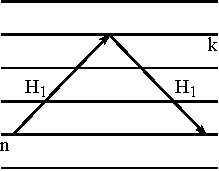
\includegraphics{419Ubergang}
\end{center}
Ist $E_k > \Braket{n | H | n}$, der Zustand also klassisch unerreichbar, so spricht man von einem \emph{virtuellen Effekt.}

Mit \emph{Pr"azisionsmessungen } kann man Zust"ande $\ket {k^{(0)}}$ erforschen, selbst wenn $E_k^{(0)}$ f"urs Experiment unerreichbar ist.

$\leadsto$ Wichtig f"ur Teilchenphysik.

\subsection{Entartete St"orungstheorie}

$E_n{(0)}$ sei $N$-fach entartet
\eqn{H_0 \ket{ n^{(0)} \alpha} & = E_n^{(0)} \ket{n^{(0)} \alpha \quad \mathrm{ mit \ } \alpha =1, \ldots,N}} 
Entarteter $N$-dimensionaler Unterraum:
\eqn{
 & \mathcal E:= \left[ \set{ \ket{ n^{(0)}\alpha} } \right] \\
&\Braket{ n^{(0)} \alpha | n^{(0)} \beta }  = \delta_{\alpha \beta}
}
Jede Linearkombination 
\eqn{ \ket{ n^{(0)} \gamma } & = \sum_{\alpha=1}^N \ket{n^{(0)} \alpha } c_{\alpha \gamma}}
mit $c_{\alpha \gamma} \in \CC$ ist ebenfalls Eigenket von $H_0$ zu $E_n^{(0)}$.

Wir w"ahlen denselben Ansatz wie im nichtentarteten Fall in Gl. (404), (406)-(411).

Mit der Entartung $\ket n \longrightarrow \ket{ n \gamma}$ wir (409) zu:
$$(H_0 - E_n^{(0)}) \ket{ n^{(1)} \gamma} = - (H_1 - E_n^{(1)}) \ket{n ^{(0)} \gamma}$$
Linksmultiplikation mit $\ket{n^{(0)} \beta}$ ergibt
\eqn{ 0 = - \Braket{n^{(0)} \beta | H_1 - E_n^{(1)} | n^{(0)} \gamma}}
also ist (423):
\eqn{ \sum_{\alpha=1}^N c_{\alpha \beta} \braket{ n^{(0)} \beta | H_1 | n^{(0)} \alpha } & = E_n^{(1)} c_{\beta \gamma}}
Matrixdarstellung:
\eqn{ {h_1}_{\beta \alpha} &  = \Braket{ n^{(0)} \beta | H_1 | n^{(0)} \alpha}}
(425) $\Longrightarrow$
\eqn{ \sum_{\alpha=1}^N {h_1}_{\beta \alpha} C_{\alpha_\gamma} & = E_n^{(1)} c_{\beta \gamma}}
Eigenwertproblem einer $N \times N$ Matrix.
$\Longrightarrow$
\eqn{\det \left( h_1 - E_n^{(1)} \right) & = 0}
(428) hat $N$ L"osungen $E_{n\gamma^{(1)}}$, die nicht alle verschieden sein m"ussen. Die zugeh"origen Eigenvektoren (siehe (427)) sind
\eqn{ \vv c^\gamma := \matr{ c_{1 \gamma} \\ c_{2 \gamma} \\ \vdots \\ c_{N \gamma} }, \quad \gamma=1, \ldots, N}
mit $\left( \vv c^\gamma \right)^\dagger \vv c^{\gamma'} = \delta_{\gamma \gamma'}$. Der Basiswechsel zwischen $\ket{ n^{(0)} \alpha}$ und $\ket{ n^{(0)'} \gamma}$ in (423) diagonalisiert wegen (427) also $h_1$, die Matrix $C=(c_{\alpha \beta})$ ist unit"ar.

(427) bedeutet
\eqn{C^\dagger h_1 C = \mathrm{diag} \left( E_{n_1}^{(1)}, \ldots, E_{n_N}^{(2)} \right)}
D.h. (423) diagonalisiert mit (427) die St"orung $H_1$ im Unterraum $\mathcal E$:
\eqn{ \Braket{ n^{(0)'} \gamma | H_1 | n^{(0)'} \gamma'} = E_{n\gamma}^{(1)} \delta_{\gamma \gamma'}}
$\Longrightarrow$ Bedingung (405) "uberlistet.

Wir beobachten, dass $H_1$ die $N$-fache Entartung i.a. aufhebt (oder reduziert)
\begin{center}
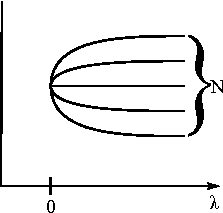
\includegraphics{431EntartRed}
\end{center}
Im Fall $E_{n \gamma}^{(1)}$ wird jedoch aus (428) bestimmt. (416) wird nun zu:
\eqn{ 
\spl{
\ket{ n^{(1)} \gamma } & = \sum_{\ket{ k^{(0)}}  \in \mathcal E} \ket{ k^{(0)}} \frac{ \Braket{ k^{(0)} | H_1 | n^{(0)} \gamma }}{E_n^{(0)} - E_k^{(0)}} + \sum_{\gamma' =1 \atop \gamma' \neq \gamma}^N \ket{ n^{(0)'} \gamma} \Braket{ n^{(0)'} \gamma' | n^{(0)'} \gamma' } \\
\ket{n^{(1)'} \gamma} & = \sum_{k \neq n} \ket{k^{(0)}} \frac{ \Braket{ k^{(0)} | H_1 | n^{(0)'} \gamma} }{E_n^{(0)} - E_k^{(0)}} + \sum_{\gamma'=1 \atop \gamma' \neq \gamma} \ket{n^{(0)'} \gamma} \Braket{ n^{(0)'} \gamma' | n^{(0)'} \gamma'}
}}
Neu: Komponenten $\Braket{ n^{(0)'} \gamma' | n^{(1)'} \gamma}$!

(410) entspricht im entarteten Fall:
\eqn{ H_1 \ket{n^{(1)'} \gamma} + H_0 \ket{ n^{(2)'} \gamma} & = E_{n\gamma}^{(2)} \ket{ n^{(1)'} \gamma} + E_{n \gamma}^{(1)} \ket{ n^{(1)'} \gamma} + E_n^{(0)} \ket{n^{(2)'} \gamma}}
Multiplikation mit $\ket{ n^{(0)'} \gamma'}$
\eqn{ \Braket{ n^{(0)'} \gamma' |  H_1 | n^{(1)'} \gamma} + E_n^{(0)} \Braket{ n^{(0)'} \gamma' | n^{(2)} \gamma} & = 
\begin{aligned}[t]
& E_{n \gamma}^{(2)} \delta_{\gamma \gamma'} + \\
& \underbrace{ E_{n\gamma}^{(1)} \Braket{ n^{(0)'} \gamma' | n^{(1)'} \gamma}}_{=0 \ \mathrm{f"ur \ } x=x' \mathrm{ \ wg.\ (415)}} + \\ 
& E_n^{(0)} \Braket{ n^{(0)'} \gamma' | n^{(2)'} \gamma}
\end{aligned}}
F"ur $\gamma = \gamma'$:
\eqn{ \spl{
E_{n \gamma}^{(1)} & \stackrel{(434)}= \braket{ n^{(0)} \gamma | H_1 | n^{(1)} \gamma} \\
& \stackrel{(432)}= \sum_{k \neq n} \frac{ \left\vert \Braket{ k^{(0)} | H_1 | n^{(0)'} \gamma} \right\vert^2 }{E_n^{(0)} - E_k^{(0)}}
}}
Der zweite (432) tr"agt nicht bei wegen
$$\Braket{ n^{(0)'} \gamma | H_1 | n^{(0)'} \gamma' } \stackrel{(431)}= \delta_{\gamma \gamma'} E_{n \gamma}^{(1)} = 0 \quad \mathrm{ f"ur \ } \gamma = \gamma'.$$
F"ur $\gamma \neq \gamma'$ liefert (434):
\eqn{ \spl{
E_{n\gamma}^{(1)} \Braket{ n^{(0)'} \gamma' | n^{(1)'} \gamma} & = \Braket{ n^{(0)'} \gamma' | H_1 | n^{(1)'} \gamma} \\
& \stackrel{(432)} = 
\begin{aligned}[t]
& \sum_{k \neq n} \frac{ \Braket{ n^{(0)'} \gamma' | H_1 | k^{(0)}} \Braket{ k^{(0)} | H_1 | n^{(0)'} \gamma}}{E_n^{(0)} - E_k^{(0)}} \\
& + \sum_{\gamma'' \neq \gamma} \underbrace{ \Braket{ n^{(0)'} \gamma' | H_1 | n^{(0)} \gamma'}}_{E_{n \gamma'}^{(1)} \delta_{\gamma' \gamma''}} \Braket{ n^{(0)} \gamma^{(1)} | n^{(1)'} \gamma} 
\end{aligned} \\
& = 
\begin{aligned}[t]
& \sum_{k \neq n} \frac{ \Braket{ n^{(0)} \gamma' | H_1 | k^{(0)}} \Braket{ k^{(0)} | H_1 | n^{(0)'} \gamma}}{E_n^{(0)} - E_k^{(0)}} \\
& + E_{n \gamma'}^{(1)} \Braket{ n^{(0)'} \gamma' | n^{(1)'} \gamma}
\end{aligned}
}}
Ist die Entartung aufgehoben, also $E_{n\gamma}^{(1)} \neq E_{n \gamma'}^{(1)}$, so liefert (436) uns die fehlenden Komponenten in (432).
\eqn{ \Braket{n^{(0)'} \gamma' | n^{(1)'} \gamma}& = \frac1{E_{n\gamma}^{(1)} - E_{n \gamma'}^{(1)}} \sum_{k \neq n} \frac{ \Braket{ n^{(0)'} \gamma' | H_1 | k^{(0)}} \Braket{ k^{(0)} | H_1 | n^{(0)'} \gamma}}{E_n^{(0)} - E_k^{(0)}}}
F"ur Zust"ande, die auch inerster Ordnung St"orungstheorie entartet bleiben (d.h. $E_{n\gamma}^{(1)} = E_{n \gamma'}^{(1)}$ f"ur $1 \leq \gamma, \gamma' \leq N' \leq N$) muss man nun im entarteten Unterraum den Operator
\eqn{H_1 \sum_{k \neq n} \frac{ \Ket{ k^{(0)} } \Bra{ k^{(0)}}}{E_n^{(0)} - E_k^{(0)}} H_1}
(siehe (436)) diagonalisieren.

Gilt $E_{n \gamma}^{(2)} \neq E_{n \gamma}^{(2)}$, so liefert die Ordnung $\lambda^3$ die Koeffizienten in (437).

Das Verfahren kann man zu beliebig hohen Ordnungen treiben.

\subsection{Anwendung: Feinstruktur des Wasserstoffspektrums}

\setcounter{equation}{287}
\eqn{
& \vv J = \vv L + \vv S \\
& \left[ L_j, S_k \right] = 0
}
\setcounter{equation}{438}
Gemeinsame EZ von $\vv L^2, \ L_3, \  \vv S, \ S_3$:
\eqn{ \Ket{ l \, m_l \, s \, m_s}}
Auch:
$$\left[ \vv J^2 , \vv L^2 \right] = \left[ \vv J^2, \vv S^2 \right] = 0$$
$\Longrightarrow$ Betrachte Basis aus gemeinsamen EZ von $\vv J^2, \ J_3, \ \vv L^2, \ \vv S^2$:
\eqn{ \Ket{ j \, m \, l \, s }}
Wegen $J_3 = L_3 + S_3$ ist $\Ket{ l \, m_l \, s \, m_s}$ EZ von $J_3$ zum EW $m=m_l + m_s$:
\eqn{J_3 \Ket{ l \, m_l \, s \, m_s } & = (L_3 + S_3) \Ket{ l\,m_l\, s\,m_s} = (m_l + m_s) \Ket{ l \, m_l\, s \, m_s}}
D.h. $\Ket{ j \, m \, l \, s}$ in (440) ist LInearkombination aus $\Ket{ l \, m_l \, s \, m_s}$ mit $m = m_l + m_s$.
\eqn{ \Ket{ j \, m \, l \, s} & = \sum \Ket{ l \, m_l \, s \, m_l } \underbrace{ \Braket{ l \, m_l \, s \, m_s | j \, m \, l \, s }}_{\mathrm{Clebsch-Gordan-Koeff.}} \\
j=m_{\mathrm{max}}&  = \max_{\vert m_l \vert \leq l \atop \vert m_s \vert \leq s } (m_l + m_s) \leq {m_{l}}_{\mathrm{max}} + {m_s}_{\mathrm{max}} = l +s }
Betrachte $L_3 = J_s - S_3$ und $m_s \rightarrow -m_s$
\eqn{ l = {m_l}_\mathrm{max} \leq {m_j}_\mathrm{max} - {m_s}_\mathrm{max} \leq j + s}
(443) und (444) (und die spezielle Betrachtung von $l=0$) $\Longrightarrow$
\eqn{ \vert l - s\vert \leq j \leq l +s \quad \mathrm{(Auswahlregel)}}
d.h. CG-Koeffizienten, die (445) verletzen, sind gleich null.

Ausgehend von $\Ket{ j \, j \, l \, s} = \Ket{ l \, l \, s \, s}$ berechnet man die CG-Koeffzienten in (442) mit Hilfe von $J_- = L_- + S_-$.

Wasserstoff:
$$H = H_0 + H_1$$
Relativistische Korrekturen:
\eqn{H_1 & = {H_1}_{\vv L \cdot  \vv S} + {H_1}_\mathrm{kin} + {H_1}_\mathrm{pot} \\
{H_1}_{\vv L \cdot \vv S} & = \frac1{2 m^2 c^2} \vv S \cdot \vv L \frac{ \gamma}{R^3} \quad \mathrm{hei"st \ Spin-Bahn-Kopplung} \\
\vv S \cdot \vv L & = \frac12 \left[ \left( \vv L + \vv S \right) - \vv L^2 - \vv S^2 \right] = \frac12 \left[ \vv J^2 - \vv L^2 - \vv S^2 \right]}
Die Eigenkets $\Ket{ n \, j \, m \, l \, s}$ von $H_0$ erf"ullen
\eqn{ H_0 \Ket{ n_j \, m \, l \, s} & = E_n^{(0)} \Ket{ n_j \, m \, l \, s}}
mit 
\eqnnon{E_n^{(0)} & \stackrel{(390)}= \frac{mc^2 \alpha^2}{2 n^2}}
Die St"orung ${H_1}_{\vv L \cdot \vv S}$ ist in der Basis $\set{ \Ket{ n_j \, m \, l \, s}}$ im entarteten Hilbertraum bereits diagonal, denn
\eqn{ \spl{
\Braket{ n_j' \, m' \, l' \, s' | {H_1}_{\vv L \cdot \vv S} | n_j \, m \, l \, s } & \stackrel{(448)}= \frac{\gamma}{4m^2c^2} \Braket{ n_j' \, m' \, l' \, s' | \frac1{R^3} \left( \vv J - \vv L - \vv S^2 \right) | n_j \, m \, l \, s } \\
& = \begin{aligned}[t]
\frac{ \gamma}{4 m^2 c^2} \left[ j(j+1) - l(l+1) - \frac34 \right] \delta_{jj'} \delta_{ll'} \delta_{mm'} \delta_{ss'} \\ \cdot\Braket{ n_j \, m \, l \, s | \frac1{R^3} | n_j \, m \, l \, s}
\end{aligned}
}}
F"r $l\geq 1$:
\eqn{{E_n}_{\vv L \cdot \vv S}^{(1)} & = \frac{ \gamma \hbar^2}{4 m^2 c^2 }\left[ j(j+1) - l(l+1) - \frac34 \right] \Braket{ \frac 1 r^3}_{nl}}
wobei
\eqn{
\Braket{ \frac1{r^3} }_{nl} & = \int_0^\infty \dd r \, \frac{f_{nl}^2(r)}{r} \stackrel{(396)} = \frac 2{a^3 n^3 l (l+1) (2l+1)}
}
Einsetzen in (451) liefert:
\eqn{
{E_n}_{\vv L \cdot \vv S}^{(1)} & = \underbrace{ \frac{ \gamma \hbar^2}{2 m^2 c^2 n^3 a^3}}_{\stackrel{(389),(399)}= -E_n^{(0)} \frac{\alpha^2}n} 
\begin{cases}
- \frac1{(j+1)(2j+1)}, & l=j+\frac12 \\
\frac1{j(2j+1)}, & l=j-\frac12 \neq 0
\end{cases}
}
f"ur $l=0$ ist $j=s=\frac12$, also $\underbrace{ j(j+1) - l(l+1)}_{=\frac34} - \frac34 = 0$. $\Longrightarrow$
\eqn{ {E_n}_{\vv L \cdot \vv S}^{(1)} = 0 \quad \mathrm{f"ur \ } l=0}
In (446) folgt ${H_1}_\mathrm{kin}$ aus:
\eqn{
\spl{
E & = \sqrt{m^2 c^4 + p^2 c^2} \\
& = mc^2 + \frac {p^2}{2m} - \frac18 {p^4}{m^3c^2} + \ldots \\
}  \\
\spl{
{H_1}_\mathrm{kin} & = - \frac18 \frac{P^4}{m^3c^2} \\
& = -\frac1{2mc^2} \left( \frac{pP2}{2m} \right)^2 \\
& = - \frac1{2mc^2} \left( H_0  + \frac \gamma R \right)^2
}
}
Wegen 
\eqn{ \left[ {H_1}_\mathrm{kin}, \vv J^2 \right] = \left[ {H_1}_\mathrm{kin}, J_3 \right] = \left[ {H_1}_\mathrm{kin}, \vv L^2 \right] = \left[ {H_1}_\mathrm{kin} , \vv J^2 \right] = 0}
ist ${H_1}_\mathrm{kin}$ in der Basis $\set{ \Ket{ j \, m \, l \, s }}$ diagonal.
$\Longrightarrow$
$${E_n}_\mathrm{kin}^{(1)} = \Braket{ n_j \ m \, l \, s | {H_1}_\mathrm{kin} | n_j \ m \, l \, s}.$$
Weiter
\eqn{
{E_n}_\mathrm{kin}^{(1)} & \stackrel{(456)}= - \frac1{2mc^2} \Braket{ n_j \ m \, l \, s | H_0^2 + 2 \gamma H_0 \frac 1R + \gamma^2 \frac1{R^2} | n_j \ m \, l \, s}}
Wir ben"otigen
\eqn{ \spl{
\Braket{ n_j \ m \, l \, s | \frac 1R | n_j \ m \, l \, s} & = \frac1{an^2} \\
\Braket{ n_j \ m \, l \, s | \frac 1{R^2} | n_j \ m \, l \, s} & = \frac1{a^2n^3(l+\frac12)}
}}
$\Longrightarrow$
\eqn{ 
{E_n}_\mathrm{kin}^{(1)} & = - \frac1{2mc^2} \left\{ {E_n^{(0)}}^2 + \frac{2 \gamma}{an^2} E_n^{(0)} + \frac{\gamma^2}{a^2n^2(l+\frac12)} \right\} \notag\\
& \stackrel{(389), (399)}= - E_n^{(0)} \left\{ - \frac{\alpha^2}{4n^2} + \frac{\alpha^2}{n^2} - \frac{\alpha^2}{n} \frac1{l +\frac12} \right\} \notag \\
& = - E_n^{(0)} \frac{\alpha^2}n \left\{ \frac3{4n} - \frac1{l+\frac12} \right\} \\
& = - E_n^{(0)} \frac{\alpha^2}n \left[ \frac3{4n} + \begin{cases} - \frac1{j+1}, & l=j+\frac12 \\ - \frac1j, & l=j-\frac12 \end{cases} \right]
}
Summe aus (461) und (453):
\eqn{{E_n}_{\vv L \cdot \vv S}^{(1)} + {E_n}_\mathrm{kin}^{(1)} & = - E_n^{(0)} \frac \alpha n \left[ \frac3{4n} - \frac1{j+\frac12} \right] \quad \mathrm{f"ur \ } l \geq 1}
F"ur $l=0$ folgt aus (460) und (454):
\eqn{ {E_n}_{\vv L \cdot \vv S}^{(1)} + {E_n}_\mathrm{kin}^{(1)} = {E_n}_\mathrm{kin}^{(1)} = - E_n^{(1)} \frac{\alpha^2}n \left[ \frac3{4n} - 2 \right]}
Letzter Term in (446):

Ortsdarstellung:
\eqn{
\spl{ 
{H_1}_\mathrm{pot} & = \frac{\hbar^2}{8m^2 c^2} \Delta V(r) \\
& = \frac{\pi \hbar^2 \gamma}{2 m^2 c^2} \delta^{(3)}(\vv x)
} \\
\spl{
{E_n}_\mathrm{pot}^{(1)} & = \Braket{ n_j \ m \, l \, s | {H_1}_\mathrm{pot} | n_j \ m \, l \, s } \\
& = \frac{\pi \hbar^2 \gamma}{2m^2 c^2} \vert f_{nl}(0) \vert^2 \\
& = \frac{mc^2 \alpha^4}{2n^3} \delta_{l0} \\
& = - E_n^{(0)} \left( - \frac{\alpha^2}n \right) \delta_{l0}
}
}
Summe von (463) und (465):
\eqn{ 
{E_n}^{(1)}_{\vv L \cdot \vv S} + {E_n}_\mathrm{kin}^{(1)} + {E_n}_\mathrm{pot}^{(1)} & = \begin{cases} \displaystyle- E_n^{(0)} \frac{\alpha^2}n \left[ \frac3{4n} - 1 \right], & \mathrm{f"ur \ } l=0, \\
\displaystyle -E_n^{(0)} \frac{\alpha^2}n \left[ \frac3{4n} - \frac1{j+ \frac12} \right], & \mathrm{f"ur \ } l \neq 0 \end{cases}}
denn $l=0$ impliziert $j=\frac12$.

Also gilt mit (465), (466) \emph{unabh"angig} von $l$:
\eqn{\spl{
E_n^{(1)} & = -{E_n}^{(0)}_{\vv L \cdot \vv S} + {E_n}_\mathrm{pot}^{(1)} + {E_n}_\mathrm{kin}^{(1)} \\
& = - E_n^{(0)} \frac{\alpha^2}n \left[ \frac3{4n} - \frac1{j+\frac12} \right]
}}
Energie-Niveaus:
\eqn{E_{n_j} & = E_n^{(0)} + E_{n_j}^{(1)} = - \frac{mc^2}{2} \frac{\alpha^2}{n^2} \left[ 1 - \frac{\alpha^2}{n^2} \left( \frac34 - \frac n{j+\frac12} \right) \right]}
$\alpha \approx 5,4 \cdot 10^{-5}$ $\Longrightarrow$ Feinstruktur.

Relativistische Wellengleichung des Elektron: \emph{Dirac-Gleichung}

Exakt l"osen f"ur das Wasserstoff-Atom, Quantenahl $j, \, l, \, s$ sind keine guten Quantenzahlen.

\section{Streutheorie}

\begin{center}
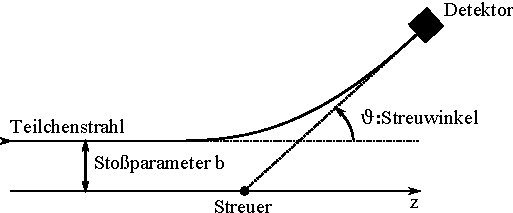
\includegraphics{469Streu}
\end{center}
Streuer: Ursprung aus dem Ubekannten, zu erforschendes Potenzial.

Einlaufender Teilchenstrahl: Stromdichte $\vv{j_\mathrm{ein}}(\vv x)$:
\eqn{ dN = \vv j d \vv F \dd t}
Teilchen str"omen in der Zeit $dt$ durch das Fl"achenelement $d \vv F ( = \vv n dF)$.

F"ur gro"se $r= \vert \vv x \vert$ verhalten sich die Teilchen fast wie freie Teilchen (gerade Trajektorien). Dann ist die Definition des differenziellen Wirkungsquerschnitts bzw. diff. Streuquerschnitt $\frac{d \sigma}{d \Omega}$ sinnvoll:
\eqn{ \frac{d\sigma}{d\Omega} = \frac1{j_\mathrm{ein}} \frac{dN}{d\Omega d t}}
\begin{center}
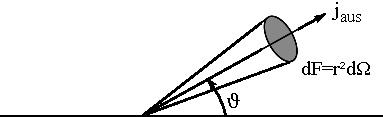
\includegraphics{470wirkquer}
\end{center}

\end{document}
